% ------------------------------------------------------------------------------
% Results
% ------------------------------------------------------------------------------

\renewcommand{\arraystretch}{1.3}
\definecolor{gray1}{RGB}{248, 249, 250}
\definecolor{gray2}{RGB}{233, 236, 239}

\chapter{Results}\label{chap:results}
	
	Chapter 5 presents the results of the computational experiments conducted in this thesis, evaluating the proposed methodologies through both case studies and benchmarking. The case studies are detailed in Section \ref{chap:results:casestudy}, which encompasses various problem scenarios, including single scatterers (subsection \ref{chap:results:casestudy:austria}), multiple scatterers (subsection \ref{chap:results:casestudy:multiple}), non-homogeneous scatterers (subsection \ref{chap:results:casestudy:nonhomogeneous}), and strong scatterers (subsection \ref{chap:results:casestudy:strong}). In each case study, a comparison is made between the proposed algorithms and traditional deterministic methods.
	
	Following the case studies, Section \ref{chap:results:benchmark} focuses on the benchmarking study, which aims to assess the performance of the proposed methods and identify any potential differences among them. The subsection \ref{chap:results:benchmark:considerations} introduces the settings of the benchmarking study, providing essential context for the subsequent analysis. Subsequently, the results are presented and discussed, offering insights into the performance of the algorithms.
	
	Some general comments apply to both the case studies and benchmarking stages. Firstly, all designs utilized lossless materials. Additionally, the amplitude of the incident wave was consistently set at 1 [V/m]. To incorporate a level of realism, the scattered field data was subjected to random noise. This noise is a random complex number, with its modulus representing a percentage of the original value and its phase uniformly distributed between $0$ and $2\pi$.
	
	Regarding runtime results, they were obtained using a specific machine configuration: Ubuntu 20.04.5 LTS, Intel Xeon(R) CPU E5-2640 0 @ 2.50GHz with 8 cores, and 11.7 GB memory. It is important to note that the method implementations may not have been optimized to their fullest extent, potentially impacting runtime analysis fairness. Consequently, a completely fair runtime analysis cannot be guaranteed due to potential variations in implementation optimizations.

	\section{Case Studies}\label{chap:results:casestudy}
		
		
		Case studies involve a comprehensive analysis of either a single or a set of specific instances of a problem. The aim is to deeply analyze these instances, carefully examining their unique attributes. These instances are deliberately chosen to explore specific characteristics that hold relevance for the proposal. By examining these selected cases, valuable insights and understanding can be gained.
		
		This section covers four case studies, each focusing on a different scenario. The first case study examines the behavior of the proposed algorithms in situations that can be easily solved using traditional methods. The second case study investigates the performance of the proposed algorithms in a scenario with multiple scatterers and a significant level of contrast. In the third case study, the objective is to analyze the behavior of the proposed algorithms when dealing with a non-homogeneous scatterer that exhibits different levels of contrast. Additionally, this case explores the capability of the qualitative method to provide suitable initial solutions in such scenarios. The fourth and final case study aims to observe the performance of the proposed algorithms in a scenario where traditional methods typically struggle to produce satisfactory solutions.
		
		Throughout all the tests, a noise level of 20 [\%/sample] is considered for the scattered field data. Such noise level might affect significantly the performance of some methods and, therefore, the goal is to analyze the performance under a challenging scenario. In addition to the five proposed algorithms discussed in Chapter \ref{chap:proposed-methodology}, an evolutionary algorithm that transforms the inverse problem into a two-dimensional optimization problem will also be included. However, this algorithm does not employ surrogate models. Furthermore, four deterministic methods, namely ECSI (Subsection \ref{chap:methods:deterministic:csi}), SOM (Subsection \ref{chap:methods:deterministic:som}), BIM (Subsection \ref{chap:methods:deterministic:bim}), and DBIM (Subsection \ref{chap:methods:deterministic:dbim}), will be employed. The ECSI version \cite{berg1999extended} of the CSI family of algorithms is chosen due to its slightly better performance and fewer control parameters.
		
		For the algorithms assisted by surrogate models, the threshold variable ranges from 0 to 1. The Method of Moments CG-FFT (MoM-CG-FFT) used in the simulations employs a stopping criterion of a maximum of 20 iterations or an error tolerance level below $10^{-3}$. This choice allows for a rougher approximation and helps to save computational time.
		
		The performance of the algorithms will be primarily analyzed based on the error in estimating the object contrast and recovering its shape. Hence, the $\zeta_{\epsilon OE}$ and $\zeta_S$ indicators will be measured, respectively. The decision not to use the $\zeta_{\epsilon PAD}$ indicator is motivated by the fact that the thresholding operator employed in the proposed approach ensures a noise-free background. This could heavily favor the proposed approach and make the comparison with traditional methods less meaningful. Lastly, the maximum number of iterations for each algorithm is determined based on the convergence of their objective function or the point just before a divergence behavior is observed.
	
		\subsection{Austria Profile}\label{chap:results:casestudy:austria}
		
			% 1. A instância utilizada neste estudo de caso é o perfil Austria, muito utilizado na literatura \citep{chen2010subspace,chen2017}.
			% 2. O objetivo do estudo de caso é testar os algoritmos num cenário de um espalhador fraco (DNL = 0.694).
			% 3. Outras características desse perfil é que são múltiplos espalhadores, sendo um deles vazado. Mais informações sobre a parametrização do problema podem ser encontrados em \citep{chen2010subspace}. A configuração do problema pode ser visualizado na Tabela \ref{tab:results:casestudy:austria:configuration}. O comprimento de onda de fundo ($\lambda_b$) para a configuração vale 0.749 [m].
			% 4. O perfil pode ser visualizado atráves da Fig. \ref{fig:results:casestudy:austria:reconstruction:groundtruth}.
			% 5. Os dados foram sintetizados através do Método dos Momentos CG-FFT (MoM-CG-FFT) cujo critério de parada foi 15000 iterações ou nível de tolerância do erro menor que $10^{-5}$. A resolução da imagem original foi de 64x64. A resolução da reconstrução será 30x30.
			
			The present case study considers the Austria profile, which is a widely used instance in the literature \citep{chen2010subspace,chen2017}, to test the algorithms in a weak scattering scenario (DNL $= 0.694$). The profile has multiple and homogeneous scatterers, one of which is hollow. The Fig. \ref{fig:results:casestudy:austria:reconstruction:groundtruth} shows the ground-truth image and further information regarding the parameters of the scatterers can be found in \citep{chen2010subspace}. The Table \ref{tab:results:casestudy:austria:configuration} shows the parameters regarding the measurement and imaging domains and the incident field configuration. The resulting background wavelength is 0.749 [m]. Scattered field data was synthesized using MoM-CG-FFT, with a stopping criterion of 15,000 iterations or error tolerance level less than $10^{-5}$, and the resolution of the original image was 64$\times$64, while the reconstruction resolution was 30$\times$30.
		
			\begin{table}[!h]
				\centering
				\caption[Parameters for Austria profile case study.]{Parameters for problem specification of Austria profile case study.}
				\rowcolors{1}{gray2}{gray1}
				\begin{tabular}{cccccc}
					$N_M$ & $N_S$ & $R_O$ & $f$ & $L_X$, $L_Y$ & $\epsilon_{rb}$ \\
					32 & 16 & 6 [m] & 400 [MHz] & 2 [m] & 1
				\end{tabular}
				\label{tab:results:casestudy:austria:configuration}
			\end{table}

			%1. O intervalo da variável de contraste foi definido como 0 a 1.
			%2. O critério de parada será definido pelo número máximo de avaliações, o qual será de 26 avaliações.
			%3. Cada algoritmo assistido por modelo substituto será executado 30 devido às características estocásticas neles presentes.
			%4. A quantidade de soluções amostradas no começo será 16.
			%5. A operação de busca local nos algoritmos SAEA's irão acontecer de 5 em 5 gerações.
			%6. O fator de mutação $F$ presente nos processos de mutação dos algoritmos SAEA's vão ser escolhidos aleatoriamente no intervalo de 0.6 a 1.5 seguindo uma distribuição normal.
			%7. Em relação aos algoritmos SAEA1 e SAEA3, o tamanho da população foi ajustada para 20 indivíduos. Já para o algoritmo SAEA2, a população foi definida em 5 indivíduos e 20 filhos gerados por pai. O número mais baixo de indivíduos foi escolhido para permitir um número maior de gerações. O tamanho do arquivo de soluções usadas para gerar vetores mutantes foi definido como o tamanho da população mais a metade do número de soluções na amostra.
			%8. Para avaliar as soluções nos algoritmos baseados em transformação, o resolvedor direto MoM-CG-FFT foi utilizado e seu número de iterações foi limitado em 20 ou até atingir um nível de tolerência de erro de 0.001. Em problemas de espalhadores fracos, bem poucas iterações podem ser necessárias para se fazer uma estimativa razoável.
			%8. Em relação ao SADM1, o tamanho da população no processo de busca por solução inicial foi definido em 100 indivíduos.
			%9. Em relação ao algoritmo evolutivo sem auxílio do modelo substituto, foi-se utilizado o algoritmo DE/rand/1/bin no qual o parâmetro $F$ foi ajustado em 0.5 e a taxa de cruzamento em 0.5.
			%10. Em relação ao SOM, o critério de parada estabelecido foi o número máximo de iterações igual 50 e o parâmetro de corte de autovalores foi 15.
			%11. Em relação ao CGM, o chute inicial foi definido como a solução do algoritmo do Backpropagation e o critério de parada foi definido como 40 iterações.
			%12. Em relação ao ECSI, o critério de parada foi definido como 50 iterações.
			%13. Em relação ao DBIM, o critério de parada foi 3 iterações e o método de regularização foi o de Tikhonov com parâmetro igual a 0.01. O número de iterações precisou ser mais baixo porque o algoritmo divergia com mais iterações.
			%14. Em relação ao BIM, foi a mesma coisa do DBIM mas o critério de parada foi ajustado em 10 iterações.

			The surrogate model-assisted algorithms proposed in this study have many parameters. The parameters for this case study were chosen based on a \textit{prior} analysis. The contrast variable range was set to 0 to 1, and the stopping criterion for each surrogate model-assisted algorithm was defined as the maximum number of evaluations, which was 26 evaluations, with 30 runs due to the stochastic characteristics present in them. Despite being based on deterministic choices, the SADM2 algorithm will be executed multiple times, and the rationale behind this decision will be elucidated in the upcoming case studies. The number of solutions sampled at the beginning was 16, and the local search operation in SAEAs algorithms happened every 5 generations. The mutation factor $F$ present in the mutation processes of SAEAs algorithms was randomly chosen in the range of 0.6 to 1.5 following a uniform distribution. The population size in the initial solution search process for SADM1 was set at 100 individuals. For the transformation-based algorithms, MoM-CG-FFT forward solver was used to evaluate solutions, with a limited number of iterations of 20 or until reaching an error tolerance level of 0.001. In addition to the surrogate model-assisted evolutionary algorithms, a traditional evolutionary algorithm formulation was also considered in this case study for comparison purposes. The DE/rand/1/bin formulation was chosen, with F adjusted to 0.5 and the crossing rate to 0.5.
			
			The parameter configuration of the deterministic algorithms is mostly related to the stop criteria, which includes the maximum number of iterations and the error tolerance level. The established stopping criterion for SOM was the maximum number of iterations equal to 50, with a cut-off parameter of eigenvalues set at 15. The initial guess for SOM, ECSI and CGM was defined as the solution of the Backpropagation algorithm (Subsection \ref{chap:methods:linear:backpropagation}). The stopping criterion for CGM and ECSI was set to 40 and 50 iterations, respectively. The stopping criterion for DBIM was 3 iterations, with the regularization method as Tikhonov's with a parameter equal to 0.01. Finally, BIM used the same parameters as DBIM, except for the stopping criterion, which was adjusted to 10 iterations. Both algorithms are considered the Born Approximation (Subsection \ref{chap:methods:linear:weak}) as initial guess strategy.
			
			\begin{figure}[!h]
				\centering
				\subfloat[Ground-Truth]{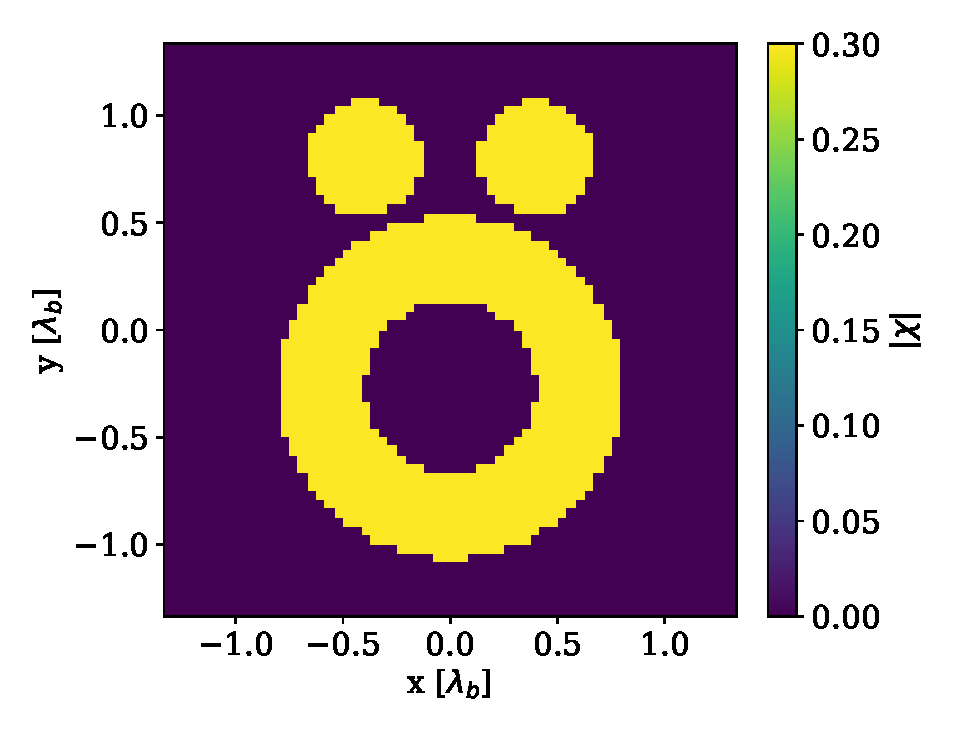
\includegraphics[width=.25\textwidth]{./figuras/casestudy/austria/groundtruth}\label{fig:results:casestudy:austria:reconstruction:groundtruth}}
				\subfloat[SAEA1]{\includegraphics[width=.25\textwidth]{./figuras/casestudy/austria/reconstruction_saea1}\label{fig:results:casestudy:austria:reconstruction:saea1}}
				\subfloat[SAEA2]{\includegraphics[width=.25\textwidth]{./figuras/casestudy/austria/reconstruction_saea2}\label{fig:results:casestudy:austria:reconstruction:saea2}}
				\subfloat[SAEA3]{\includegraphics[width=.25\textwidth]{./figuras/casestudy/austria/reconstruction_saea3}\label{fig:results:casestudy:austria:reconstruction:saea3}} \\
				\subfloat[SADM1]{\includegraphics[width=.25\textwidth]{./figuras/casestudy/austria/reconstruction_sadm1}\label{fig:results:casestudy:austria:reconstruction:sadm1}}
				\subfloat[SADM2]{\includegraphics[width=.25\textwidth]{./figuras/casestudy/austria/reconstruction_sadm2}\label{fig:results:casestudy:austria:reconstruction:sadm2}}
				\subfloat[EA]{\includegraphics[width=.25\textwidth]{./figuras/casestudy/austria/reconstruction_ea}\label{fig:results:casestudy:austria:reconstruction:ea}}
				\subfloat[BIM]{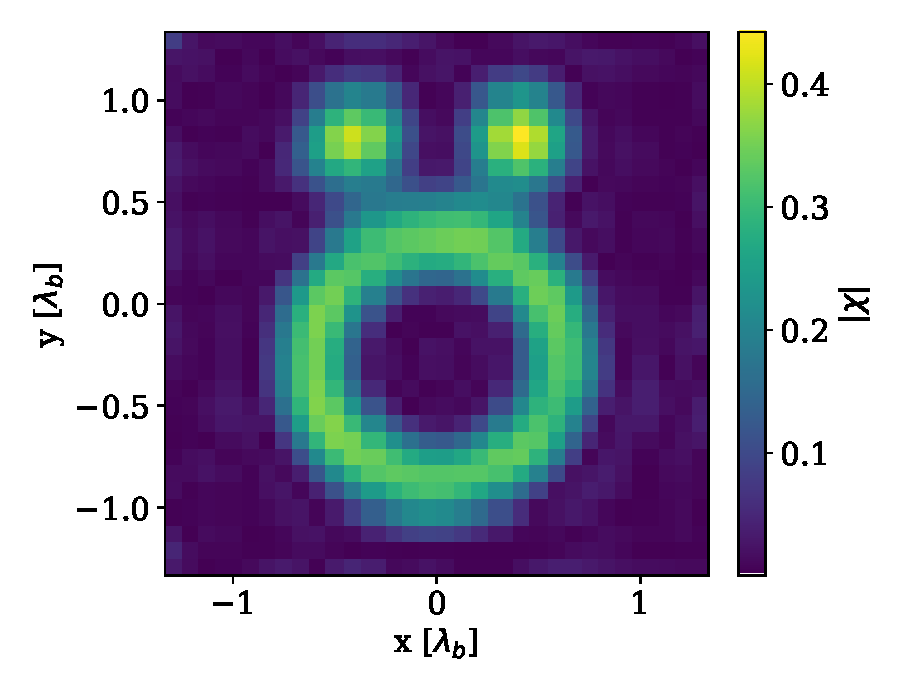
\includegraphics[width=.25\textwidth]{./figuras/casestudy/austria/reconstruction_bim}\label{fig:results:casestudy:austria:reconstruction:bim}} \\
				\subfloat[DBIM]{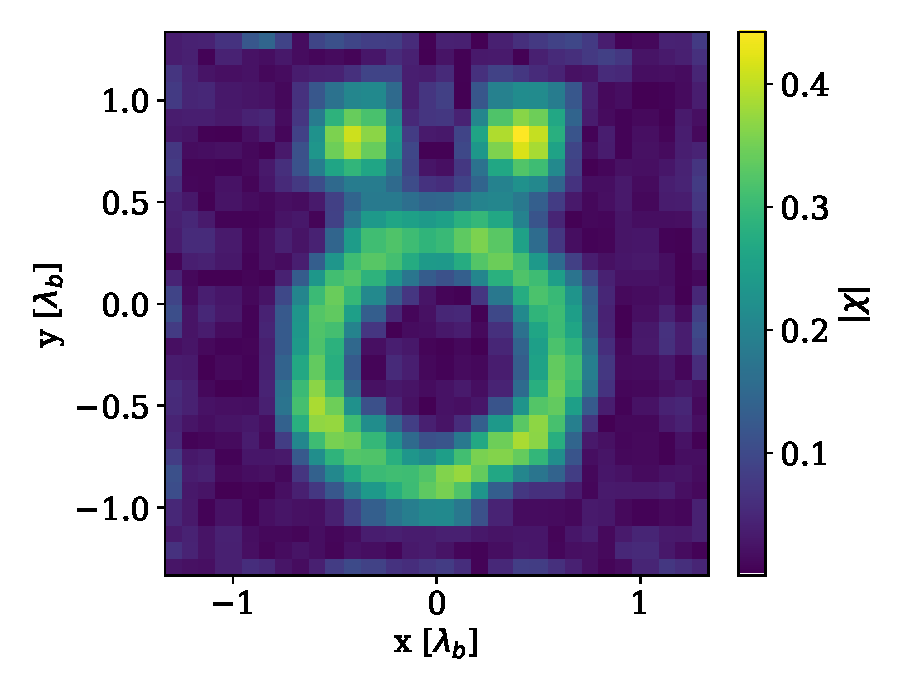
\includegraphics[width=.25\textwidth]{./figuras/casestudy/austria/reconstruction_dbim}\label{fig:results:casestudy:austria:reconstruction:dbim}}
				\subfloat[CGM]{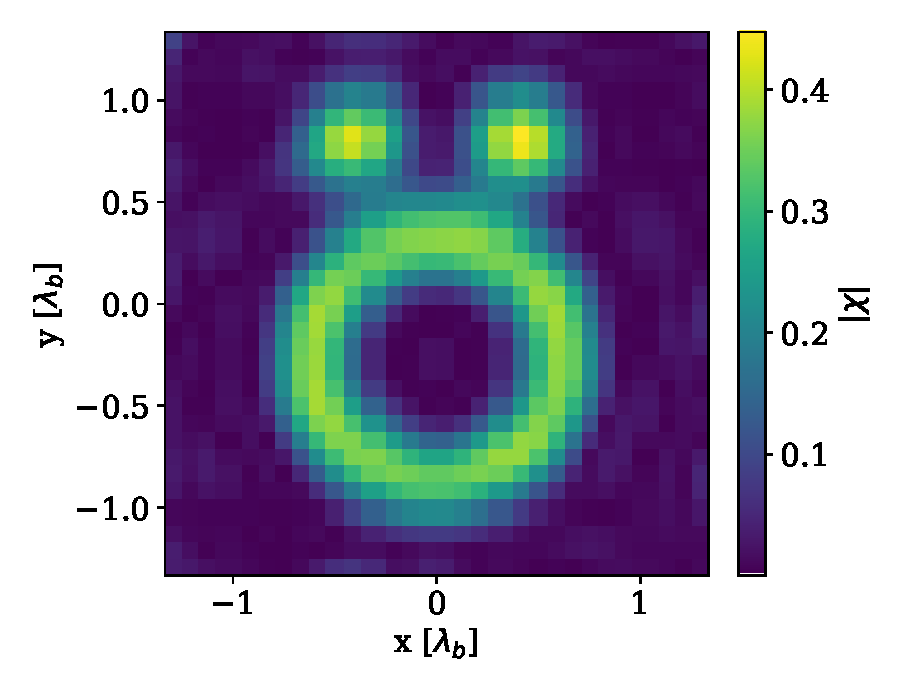
\includegraphics[width=.25\textwidth]{./figuras/casestudy/austria/reconstruction_cgm}\label{fig:results:casestudy:austria:reconstruction:cgm}}
				\subfloat[ECSI]{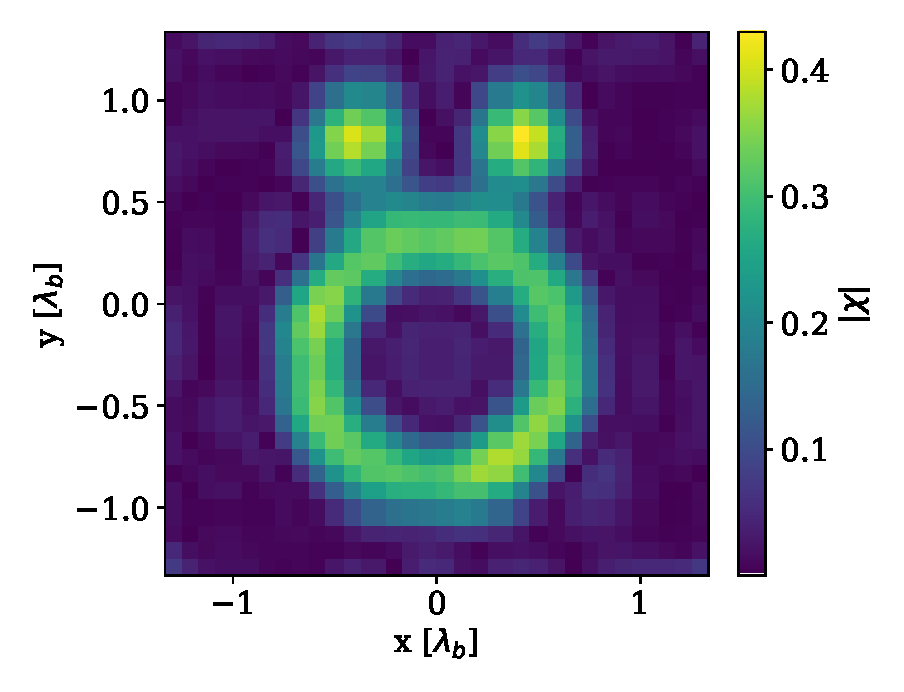
\includegraphics[width=.25\textwidth]{./figuras/casestudy/austria/reconstruction_ecsi}\label{fig:results:casestudy:austria:reconstruction:ecsi}}
				\subfloat[SOM]{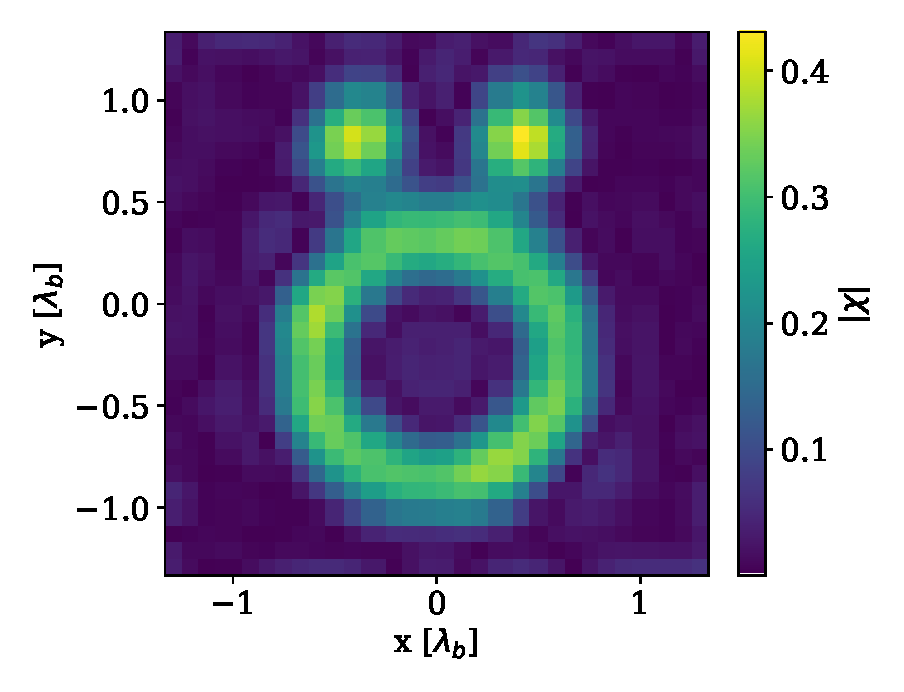
\includegraphics[width=.25\textwidth]{./figuras/casestudy/austria/reconstruction_som}\label{fig:results:casestudy:austria:reconstruction:som}} 
				\caption[Austria profile case study: Comparison of image reconstructions using surrogate model-assisted algorithms and deterministic methods.]{Comparison of image reconstructions using surrogate model-assisted algorithms and deterministic methods considering the Austria profile case study: (a) shows the ground-truth image; (b), (c), and (d) depict the best image recovered by SAEA1, SAEA2, and SAEA3, respectively, in 30 execution according to $\zeta_{\epsilon OE}$ indicator; (e), (f) and (g) show the best image recovered by SADM1, SADM2, and EA, respectively, in 30 execution according to $\zeta_{\epsilon OE}$ indicator; (g) shows the image recovered by BIM, and (h) shows the image recovered by DBIM; finally, (i), (k), and (l) show the image recovered by CGM, ECSI, and SOM, respectively.}
				\label{fig:results:casestudy:austria:reconstruction}
			\end{figure}
		
			% 1. A Fig. \ref{fig:results:casestudy:austria:reconstruction} mostra a melhor das reconstruções dentre as 30 execuções de cada algoritmo estocástico, de acordo com o indicador $\zeta_{\epsilon OE}$ (Figs. \ref{fig:results:casestudy:austria:reconstruction:saea1}-\ref{fig:results:casestudy:austria:reconstruction:ea}).
			% 2. A figura também mostra as reconstruções dos algoritmos determinísticos (Figs. \ref{fig:results:casestudy:austria:reconstruction:bim}-\ref{fig:results:casestudy:austria:reconstruction:som}).
			% 3. Todos os algoritmos fizeram uma ligeira superestimativa do contraste, conforme indica o valor máximo de contraste em cada figura. Essa suppdferestimativa tende a ser ligeiramente menor nos algoritmos baseados na proposta de transformação do problema. Este efeito tende a ser uma compensação pela subestimativa nas bordas do espalhador.
			% 4. Eles mostram também uma certa dificuldade em detectar bem a separação entre o anel e os dois círculos. Essa dificuldade está relacionada com a proximidade entre esses objetos.
			% 4. As melhores imagens reconstruídas pelo SAEA2 e pelo EA mostram um pequeno objeto fantasma dentro do anel da imagem. Isso é um problema do ajuste do valor do limiar. Como o indicador $\zeta_{\epsilon OE}$ só leva em consideração a estimativa dentro da região original do espalhador, então erros na região de fundo original do problema não são levados em conta.
			% 5. Como era de se esperar, os algoritmos baseados na transformação do problema em um de otimização bidimensional mostram uma região de fundo mais limpa. Isto é devido ao operador de limiarização. O BIM (Fig. \ref{fig:results:casestudy:austria:convergence:bim}) também apresenta uma região de fundo um pouco mais limpa que o DBIM (Fig. \ref{fig:results:casestudy:austria:convergence:dbim}) e isso está associado à dificuldade do DBIM com níveis de ruído significativos.
			
			In the results of the case study, Fig. \ref{fig:results:casestudy:austria:reconstruction} displays the best of the reconstructions among the 30 runs of each stochastic algorithm, based on indicator $\zeta_{\epsilon OE}$ (Figs. \ref{fig:results:casestudy:austria:reconstruction:saea1}-\ref{fig:results:casestudy:austria:reconstruction:ea}), and also includes the reconstructions of the deterministic algorithms (Figs. \ref{fig:results:casestudy:austria:reconstruction:bim}-\ref{fig:results:casestudy:austria:reconstruction:som}). The figures show that all algorithms overestimated the contrast slightly, which can be seen in the maximum contrast value in each figure. However, algorithms based on the problem transformation proposal tended to have slightly lower overestimation, which compensates for underestimation at the edges of the scatterer. The reconstructions also had some difficulty in detecting the separation between the ring and the two circles, which was related to the proximity between these objects. Additionally, the best SAEA2 and EA reconstructed images showed a small ghost object inside the image ring due to a threshold value adjustment issue. As the $\zeta_{\epsilon OE}$ indicator only takes into account the estimate within the original region of the scatterer, then errors in the original background region of the problem do not influence the indicator. Furthermore, algorithms based on transforming the problem into a two-dimensional optimization problem showed a cleaner background region, which was attributed to the thresholding operator. BIM (Fig. \ref{fig:results:casestudy:austria:convergence:bim}) presented a slightly cleaner background region than DBIM (Fig. \ref{fig:results:casestudy:austria:convergence:dbim}), which was associated with the difficulty of DBIM in dealing with significant noise levels.
		
			\begin{figure}[!h]
				\centering
				\subfloat[SAEA1]{\includegraphics[width=.25\textwidth]{./figuras/casestudy/austria/convergence_saea1}\label{fig:results:casestudy:austria:convergence:saea1}}
				\subfloat[SAEA2]{\includegraphics[width=.25\textwidth]{./figuras/casestudy/austria/convergence_saea2}\label{fig:results:casestudy:austria:convergence:saea2}}
				\subfloat[SAEA3]{\includegraphics[width=.25\textwidth]{./figuras/casestudy/austria/convergence_saea3}\label{fig:results:casestudy:austria:convergence:saea3}}
				\subfloat[SADM1]{\includegraphics[width=.25\textwidth]{./figuras/casestudy/austria/convergence_sadm1}\label{fig:results:casestudy:austria:convergence:sadm1}} \\
				\subfloat[SADM2]{\includegraphics[width=.25\textwidth]{./figuras/casestudy/austria/convergence_sadm2}\label{fig:results:casestudy:austria:convergence:sadm2}}
				\subfloat[EA]{\includegraphics[width=.25\textwidth]{./figuras/casestudy/austria/convergence_ea}\label{fig:results:casestudy:austria:convergence:ea}}
				\subfloat[BIM]{\includegraphics[width=.25\textwidth]{./figuras/casestudy/austria/convergence_bim}\label{fig:results:casestudy:austria:convergence:bim}}
				\subfloat[DBIM]{\includegraphics[width=.25\textwidth]{./figuras/casestudy/austria/convergence_dbim}\label{fig:results:casestudy:austria:convergence:dbim}} \\
				\subfloat[CGM]{\includegraphics[width=.25\textwidth]{./figuras/casestudy/austria/convergence_cgm}\label{fig:results:casestudy:austria:convergence:cgm}}
				\subfloat[ECSI]{\includegraphics[width=.25\textwidth]{./figuras/casestudy/austria/convergence_ecsi}\label{fig:results:casestudy:austria:convergence:ecsi}}
				\subfloat[SOM]{\includegraphics[width=.25\textwidth]{./figuras/casestudy/austria/convergence_som}\label{fig:results:casestudy:austria:convergence:som}} 
				\caption[Convergence of the objective function for the Austria profile case obtained by the stochastic and deterministic algorithms.]{Convergence of the objective function for the Austria profile case obtained by the stochastic and deterministic algorithms. (a) to (k) show the curves obtained by SAEA1, SAEA2, SAEA3, SADM1, SADM2, EA, BIM, DBIM, CGM, ECSI, and SOM algorithms, respectively. The x-axis represents the number of iterations, and the y-axis represents the value of the objective function of the correspondent algorithm.}
				\label{fig:results:casestudy:austria:convergence}
			\end{figure}
		
			% 1. A Fig. \ref{fig:results:casestudy:austria:convergence} mostra a curva de convergência da função-objetivo para cada algoritmo.
			% 2. Como cada algoritmo determinístico tem sua própria função-objetivo que pauta a sua estrutura, o eixo y só pode ser comparado entre os algoritmos baseados na otimização bidimensional (Figs. \ref{fig:results:casestudy:austria:convergence:saea1}-\ref{fig:results:casestudy:austria:convergence:ea}).
			% 3. O SAEA3 teve somente 3 gerações. O número baixo é explicado pelo fato de que cada iteração o número de avaliações da função-objetivo verdadeira é igual ao tamanho da população. Isto é diferente do SAEA1 e do SAEA3 que gastam somente uma avaliação por geração.
			% 4. Mesmo com poucas gerações, o SAEA2 ainda assim termina as execuções com valores próximos dos alcançados pelo SAEA1 e pelo SAEA3. Isso tem a ver com o bom mapeamento do espaço de busca feito pela população inicial.
			% 5. Os valores finais alcançados pelo SAEA1 nas 30 execuções foram mais semelhantes que os do SAEA3. Isto pode sugerir que a convergência do SAEA1 é melhor.
			% 6. Algumas execuções do SADM1 não convergiram para o mesmo local que a maioria. Isto pode ser um efeito do processo estocástico de busca por solução inicial. O mesmo não acontece para o SADM2. Todas as execuções desse algoritmo convergiram igualmente, indicando um comportamento determinístico.
			% 7. O EA tem mais gerações que o SAEA2 porque o EA não tem a necessidade de gerar uma amostra inicial de soluções. No entanto, o número maior de gerações não contribuiu para alcançar mais rapidamente a região perto do mínimo. Isso é mais factível para o SAEA2 por causa da estratégia de amostragem de soluções.
			
			The convergence curve for each algorithm is shown in Fig. \ref{fig:results:casestudy:austria:convergence}. The y-axis can only be compared between algorithms based on two-dimensional optimization (Figs. \ref{fig:results:casestudy:austria:convergence:saea1}-\ref{fig:results:casestudy:austria:convergence:ea}), as each deterministic algorithm has its own objective function that guides its structure. SAEA2 had a few generations but still achieved values close to those achieved by SAEA1 and SAEA3, thanks to the good mapping of the search space done by the initial population. The final values reached by SAEA1 in the 30 runs were more similar than those by SAEA3, which may suggest that SAEA1 convergence is better.
			
			Some SADM1 runs did not converge to the same location as most, which may be an effect of the stochastic search process for the initial solution. The same does not happen for SADM2, as all executions of this algorithm converged equally, indicating a deterministic behavior. The EA has more generations than the SAEA2, but the greater number of generations did not contribute to reaching the region closer to the minimum more quickly. This is straightforward for SAEA2 because of the solution sampling strategy.			
		
			\begin{figure}
				\centering
				\subfloat[]{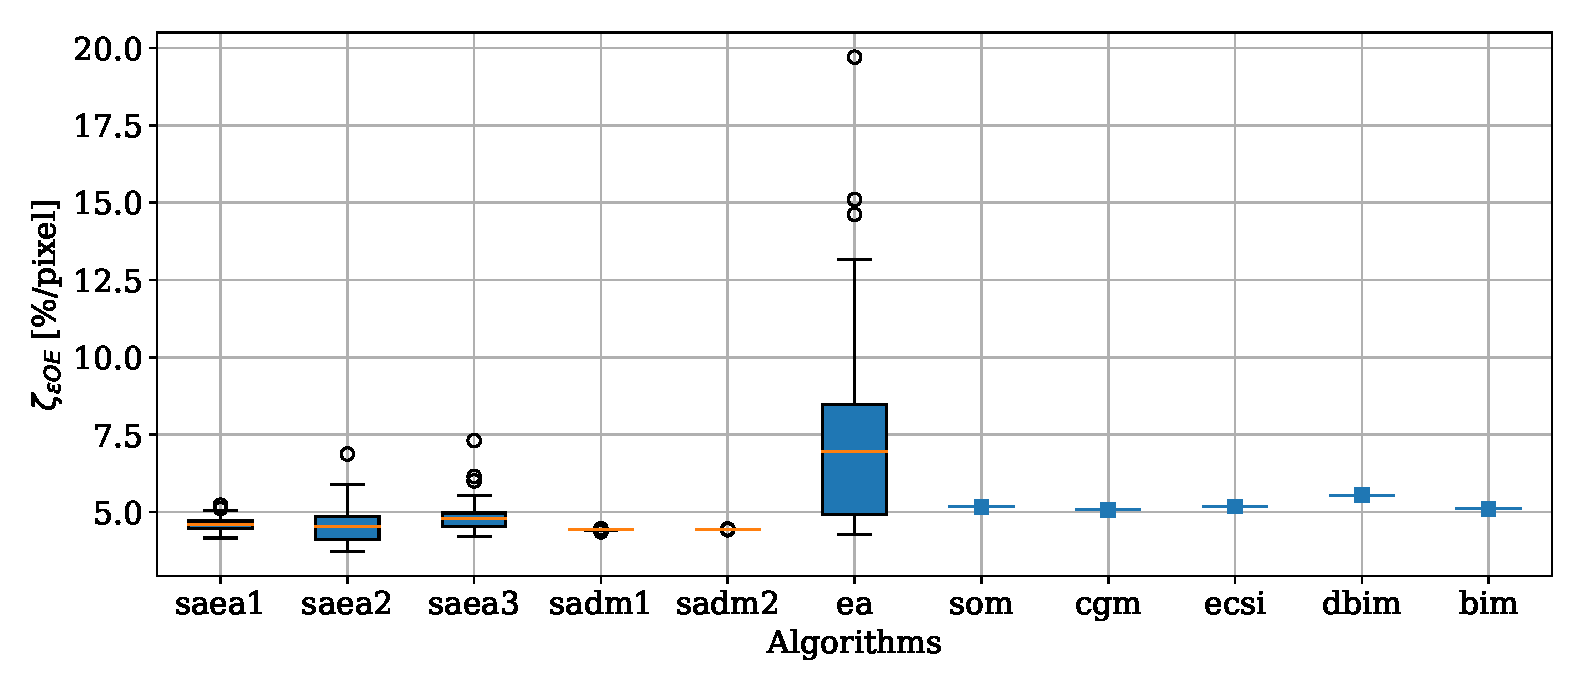
\includegraphics[width=.9\textwidth]{./figuras/casestudy/austria/boxplot_zeta_eoe_ea}\label{fig:results:casestudy:austria:boxplot:zeta_eoe:withea}} \\
				\subfloat[]{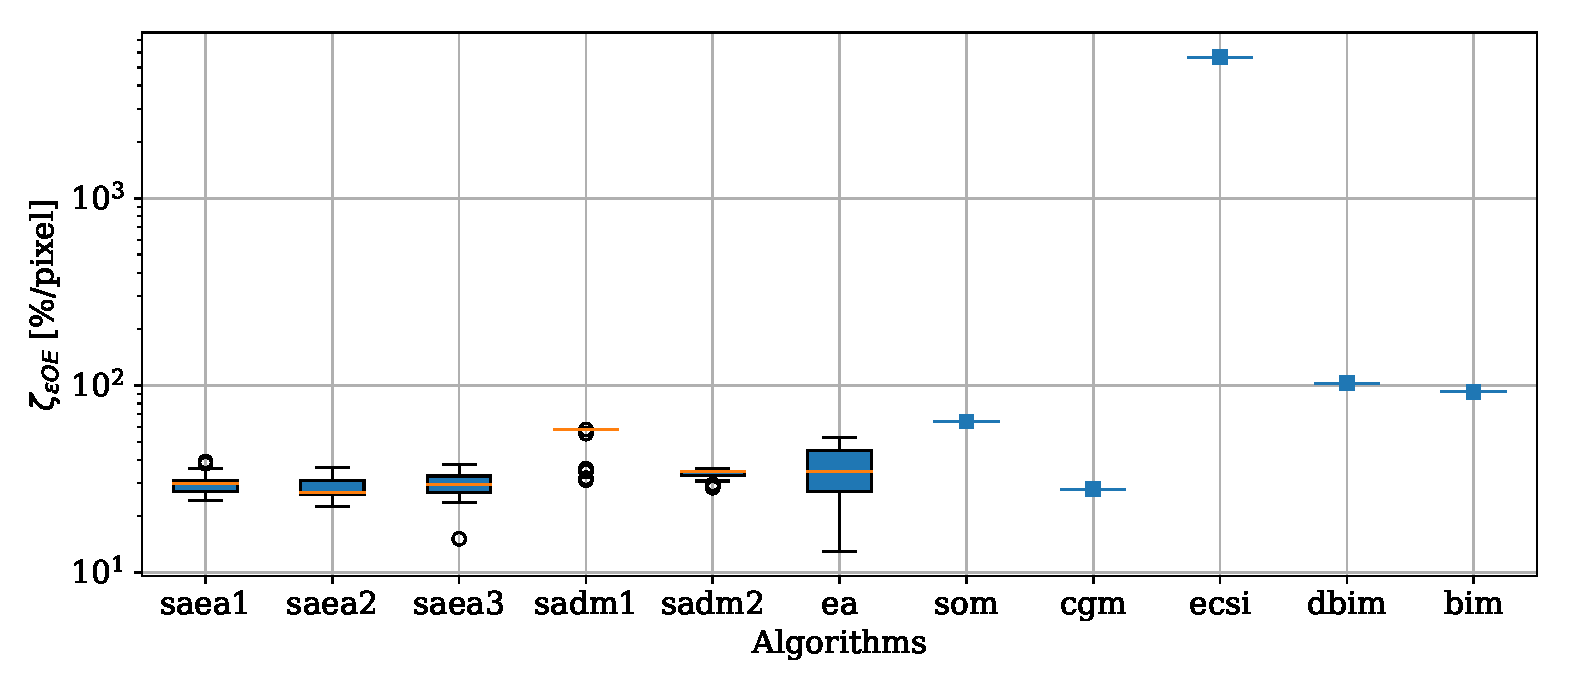
\includegraphics[width=.9\textwidth]{./figuras/casestudy/austria/boxplot_zeta_eoe}\label{fig:results:casestudy:austria:boxplot:zeta_eoe:noea}}
				\caption[Performance of $\zeta_{\epsilon OE}$ indicator for various algorithms in the Austria profile.]{Performance of $\zeta_{\epsilon OE}$ indicator for various algorithms in the Austria profile. (a) Boxplots show quartiles of 30 executions for stochastic algorithms, and the solid line represents the deterministic algorithms. (b) Exclusion of the EA algorithm for better visualization of differences among algorithms.}
				\label{fig:results:casestudy:austria:boxplot:zeta_eoe}
			\end{figure}
		
			% 1. A Fig. \ref{fig:results:casestudy:austria:boxplot:zeta_eoe:withea} mostra os quartis do indicador $\zeta_{\epsilon OE}$ para os algoritmos nos quais foram executadas 30 execuções e o valor alcançados pelos determinísticos.
			% 2. Os quartis do EA se destacam negativamente. Tal dificuldade por encontrar uma boa estimativa final do contraste do espalhador tem a ver com a necessidade que o algoritmo tem de mais gerações para poder convergir para mais perto do ótimo, como nos outros algoritmos assistidos por modelos substitutos.
			% 3. Removendo os dados do EA (Fig. \ref{fig:results:casestudy:austria:boxplot:zeta_eoe:noea}), é possível visualizar melhor as diferenças entre os algoritmos assistidos por modelos substitutos e os determinísticos. A mediana dos algoritmos assistidos por modelos substitutos ficaram abaixo de todos os determinísticos. Em especial, todas as execuções do SADM1 e do SADM2 ficaram abaixo do erro de estimativa de contraste dos determinísticos. No entanto, houveram execuções dos SAEA's que terminaram com um erro menor.
			% 4. Todas as execuções do SADM2 terminaram com o mesmo erro, uma vez que todas as execuções convergiram de igual modo (conforme visto na Fig. \ref{fig:results:casestudy:austria:convergence:sadm2}). Embora a convergência do SADM1 não tenha sido tão igual entre as execuções, eles alcançaram o mesmo erro. Isso indica que a solução final de cada execução foi muito próxima.
			% 5. O erro da estimativa de contraste dos algoritmos assistidos por modelos substitutos tem a ver com o local da superfície de otimização no qual eles terminam.
			% 6. De uma maneira geral, o resultado indica que a abordagem de transformação do problema pode ser bem sucedida de forma a fazer uma estimativa de contraste melhor na mediana dos casos, comparando com as abordagens tradicionais. No entanto, em cenários de espalhadores fracos, essa diferença não é tão significativa conforme mostra os gráficos (até 1.5 [\%/pixel]).
			
			Fig. \ref{fig:results:casestudy:austria:boxplot:zeta_eoe:withea} shows the $\zeta_{\epsilon OE}$ indicator quartiles for the algorithms in which 30 executions were performed and the value reached by the deterministic ones. The EA quartiles stand out negatively, as the algorithm has difficulty finding a good final estimate of the scatterer contrast. This is attributed to the algorithm's need for more generations to converge closer to the optimum, as in other algorithms assisted by surrogate models.
			
			By removing the EA data (Fig. \ref{fig:results:casestudy:austria:boxplot:zeta_eoe:noea}), it is possible to better visualize the differences between the algorithms assisted by surrogate models and the deterministic ones. The median of algorithms assisted by surrogate models was below all deterministic ones. In particular, all SADM1 and SADM2 runs were below the deterministic contrast estimation error. However, there have been executions of SAEA's that ended with a minor error. All runs of SADM2 ended with the same error since all runs converged equally (as seen in Fig. \ref{fig:results:casestudy:austria:convergence:sadm2}). Although SADM1 convergence was not as equal between runs, they achieved the same error, indicating that the final solution for each run was very close. The Kruskal-Wallis H-Test confirmed difference among SAEA1, SAEA2, and SAEA3 (p-value $=0.0219$), and all-to-all comparison by Mann-Whitney U test confirmed that SAEA1 and SAEA2 overperformed SAEA3 (p-values 0.0199 and 0.0191, respectively). The Multiple Mann-Whitney U test did not detected difference between SADM1 and SADM2 (p-value $=0.0505$).
			
			The contrast estimation error of surrogate model-assisted algorithms has to do with where on the optimization surface they end up. In general, the result indicates that the problem transformation approach can be successful in making a better contrast estimate in the median of cases compared to the traditional approaches. However, in weak scattering scenarios, this difference is not as significant as the graphs show (up to 1.5 [\%/pixel]).
		
			\begin{figure}
				\centering
				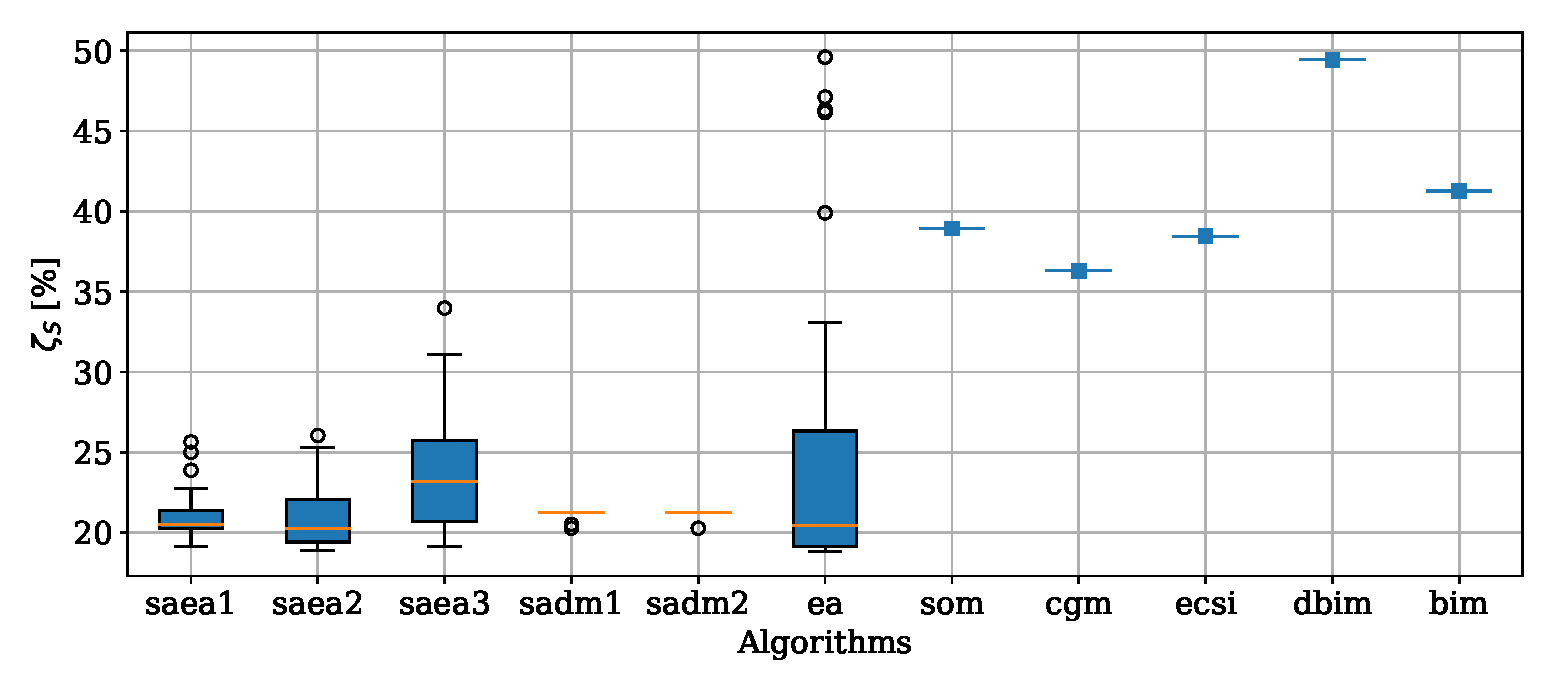
\includegraphics[width=.9\textwidth]{./figuras/casestudy/austria/boxplot_zeta_s}
				\caption[Performance of shape error estimation quantified by the $\zeta_S$ indicator obtained by the set of algorithms considering the Austria profile.]{Performance of shape error estimation quantified by the $\zeta_S$ indicator obtained by the set of algorithms considering the Austria profile. The boxes represent the quartiles of the 30 executions of the stochastic algorithms, while the other points indicate the obtained values by the deterministic ones. The shape error is calculated based on the ground-truth image and the reconstructed image obtained by each algorithm.}
				\label{fig:results:casestudy:austria:boxplot:zeta_s}
			\end{figure}
		
			% 1. Em relação ao erro de recuperação de forma $\zeta_S$ (Fig. \ref{fig:results:casestudy:austria:boxplot:zeta_s}), a diferença de desempenho é mais significativa entre os algoritmos determinísticos e aqueles baseados na transformação do problema. A diferença pode ser de até 20\%, aproximadamente, da área do espalhador original.
			% 2. O sucesso da abordagem de transformação proposta nos resultados de recuperação de forma está associado tanto à qualidade dos métodos qualitativos em fazer essa estimativa quanto na eficiência da operação de limiarização intrínseca à formulação.
			
			The performance of different algorithms for shape recovery error ($\zeta_S$) is shown in Fig. \ref{fig:results:casestudy:austria:boxplot:zeta_s}. The difference in performance between deterministic algorithms and those based on the transformation of the problem is more significant, up to approximately 20\% of the area of the original scatterer. The success of the proposed transformation approach in shape recovery results is associated with the quality of the qualitative methods used and the efficiency of the thresholding operation intrinsic to the formulation. The Kruskal-Wallis H-Test confirmed difference among SAEA1, SAEA2, and SAEA3 (p-value $<0.0002$), and all-to-all comparison by Multiple Mann-Whitney U test confirmed that SAEA1 and SAEA2 overperformed SAEA3 (p-values $<0.001$ for both cases). The Mann-Whitney U test detected difference suggesting that SADM1 outperform SADM2 (p-value $=0.013$).
		
			\begin{figure}
				\centering
				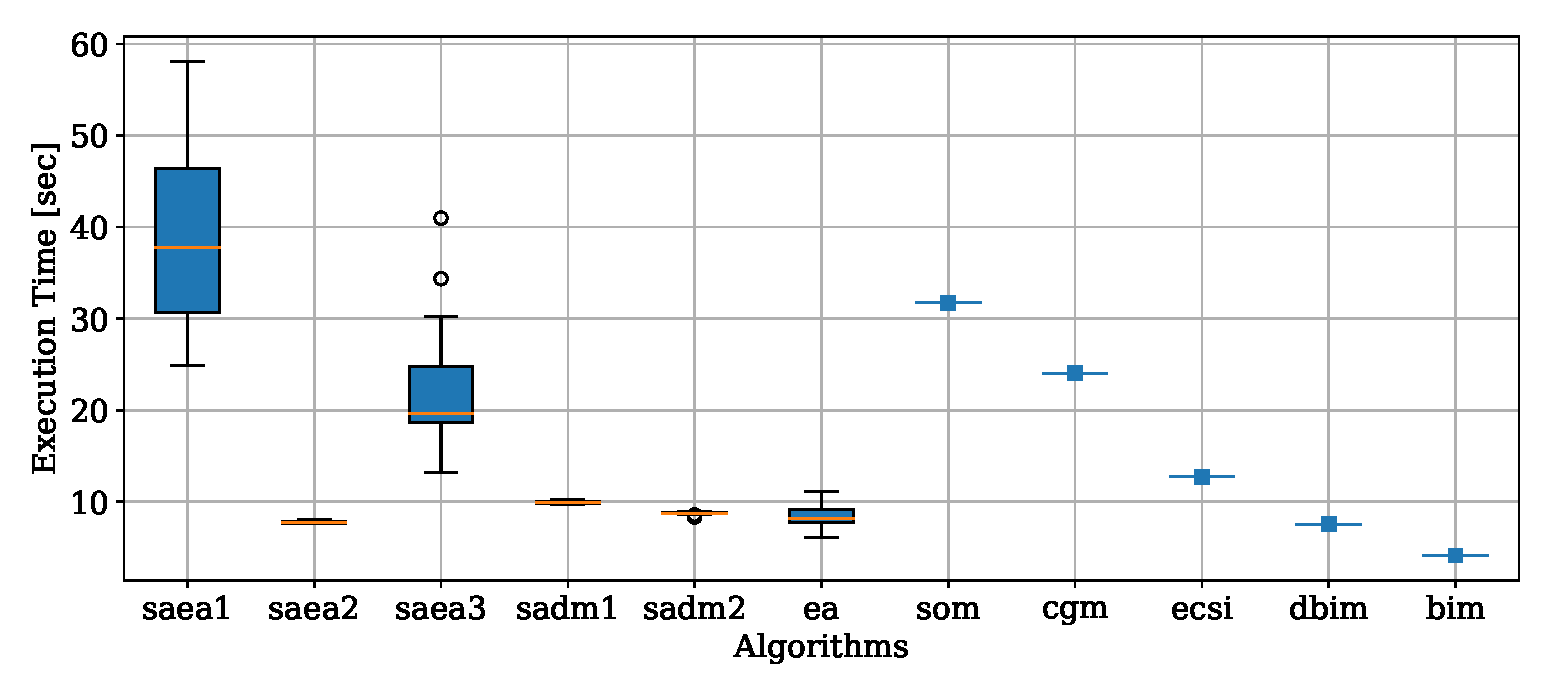
\includegraphics[width=.9\textwidth]{./figuras/casestudy/austria/boxplot_time}
				\caption[Box plot showing the execution time distribution of the set of algorithms considered for the Austria profile case.]{Box plot showing the execution time distribution of the set of algorithms considered for the Austria profile case. The boxes represent the quartiles of the 30 executions of the stochastic algorithms, and the whiskers represent the minimum and maximum values. The deterministic algorithms are represented by individual points. The execution time results are presented in seconds.}
				\label{fig:results:casestudy:austria:boxplot:time}
			\end{figure}
		
			% 1. A Fig. \ref{fig:results:casestudy:austria:boxplot:time} mostra o tempo de execução dos algoritmos.
			% 2. A mediana do SAEA1 foi a mais alta. Levando em conta somente as formulações do SAEA's, o SAEA2 foi o mais rápido, mesmo tendo o mesmo número de avaliações. Este resultado sugere o impacto de operações dentro do processo iterativo desses algoritmos, como o processo de busca local e o número de chamadas de treinamento do modelo que são menos acionados no SAEA2 para o mesmo número de avaliações.
			% 3. No entanto, vale à pena observar que os SADM's também precisam retreinar o modelo uma vez por iteração, também gastam uma avaliação por iteração e também fazem um uso do mesmo algoritmo que é aplicado para o processo de busca local no SAEA's. Logo, outros processos que fazem parte da implementação desses algoritmos também podem estar impactando o tempo de execução.
			% 4. É importante destacar também que, embora o BIM leve muito menos tempo que o SADM2, este último ainda consegue entregar bons resultados de estimativa de contraste e de forma por um tempo que é satisfatório (menor que 10 segundos) e menor que outros algoritmos como SOM, CGM e ECSI. Por isso, com um pouco mais de tempo, o SADM2 consegue entregar um resultado melhor nesta instância que é bem tratada por algoritmos tradicionais.
			
			The running time of the algorithms is shown in Fig. \ref{fig:results:casestudy:austria:boxplot:time}. The median of SAEA1 was found to be the highest, while SAEA2 was the fastest among SAEA's formulations, even with the same number of evaluations. This suggests the impact of operations within the iterative process of these algorithms, such as the local search process and the number of model training calls that are less triggered in SAEA2 for the same number of evaluations. However, it is important to note that SADMs also need to retrain the model once per iteration, spend one evaluation per iteration, and use the same algorithm applied for the local search process in SAEAs. Other processes that are part of the implementation of these algorithms may also be impacting the runtime. It is also worth highlighting that although BIM takes much less time than SADM2, the latter still manages to deliver good contrast and shape estimation results for a satisfactory time (less than 10 seconds), which is shorter than other algorithms such as SOM, CGM, and ECSI. Therefore, with a little more time, SADM2 can deliver a better result in this instance that is well-treated by traditional algorithms.
		
			\begin{figure}
				\centering
				\subfloat[]{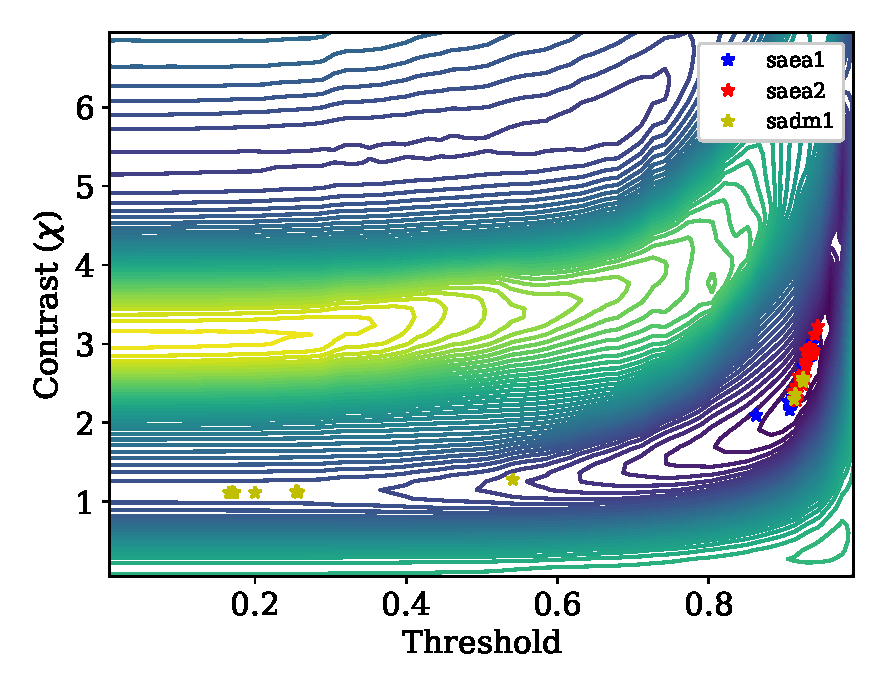
\includegraphics[width=.45\textwidth]{./figuras/casestudy/austria/surface1}\label{fig:results:casestudy:austria:boxplot:surface:1}} \hspace{.05\textwidth}
				\subfloat[]{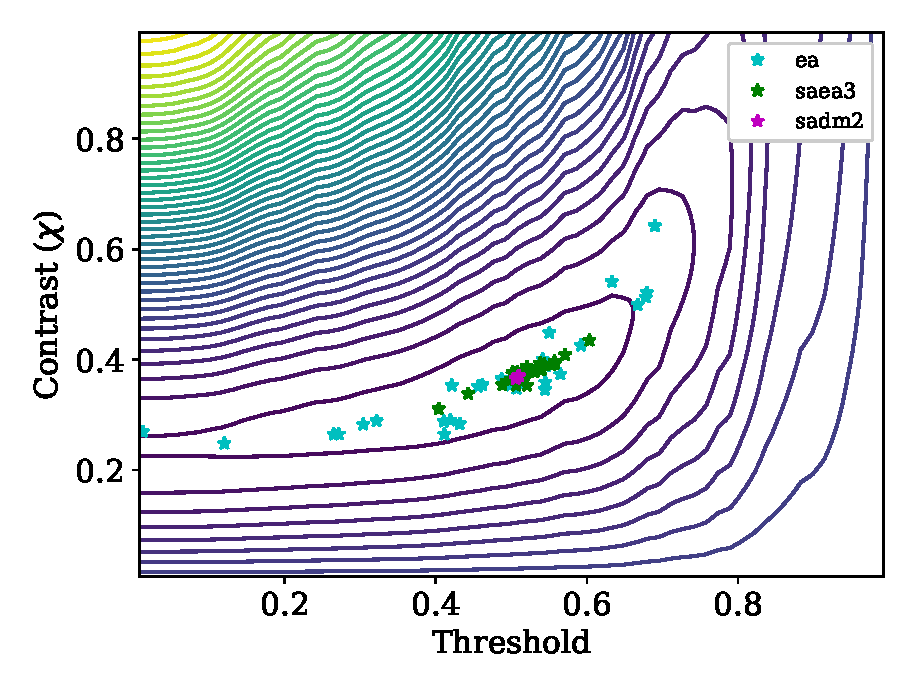
\includegraphics[width=.45\textwidth]{./figuras/casestudy/austria/surface2}\label{fig:results:casestudy:austria:boxplot:surface:2}}
				\caption[Surface of the two-dimensional optimization problem obtained from the transformation of the Austria profile and the final solutions obtained by different algorithms.]{Surface of the two-dimensional optimization problem obtained from the transformation of the Austria profile and the final solutions obtained by different algorithms. Subfigure (a) shows the final solutions obtained by SAEA1, SAEA2, and SADM1 algorithms, while subfigure (b) shows the final solutions obtained by EA, SAEA3, and SADM2 algorithms.}
				\label{fig:results:casestudy:austria:surface}
			\end{figure}
		
			% 1. A Fig. \ref{fig:results:casestudy:austria:surface} mostra a superfície da função-objetivo e a posição das soluções finais encontrada por cada algoritmo baseado na transformação do problema inverso em um de otimização bidimensional.
			% 2. Para uma superfície razoavelmente comportada no sentido macro, os SADM's se comportam como algoritmos determinísticos, uma vez que convergiram todas as vezes para o mesmo ponto.
			% 3. A figura mostra também o grande espalhamento das soluções do EA, indicando que o número de avaliações precisaria ser bem maior para que o algoritmo convergisse mais vezes para o local do ótimo.
			% 4. Os SAEA's tiveram um comportamento similar, exceto talvez pelo SAEA3 que ligeiramente se afastou mais do ponto encontrado pelos SADM's.
			% 5. É importante que soluções finais pouco mais distantes do ótimo podem retornar às vezes um erro menor de estimativa de contraste ou de recuperação de forma. Isso se dá pelo motivo que o ponto de ótimo do problema transformado pode ser um pouco deslocado daquilo que seria o ideal para o processo de limiarização e do valor exato de contraste. Esse deslocamento é intrínseco à estimativa do método qualitativo. Ou seja, a solução ótima do problema transformado não é necessariamente a exata, mas a melhor que posso obter a partir do método qualitativo e minimizando o erro da equação de dados. Por isso, a performance do método qualitativo influencia na posição do ótimo.
			
			Figure \ref{fig:results:casestudy:austria:surface} illustrates the performance of the algorithms, displaying both the objective function surface and the locations of the final solutions obtained by each algorithm after transforming the inverse problem into a two-dimensional optimization problem. The SADMs converged to the same point every time, indicating that they behaved like deterministic algorithms for a reasonably smooth surface in the macro sense. The EA solutions, on the other hand, were widely spread, indicating that the number of evaluations would need to be much higher for the algorithm to converge more often to the optimal location.
			
			The SAEA3 had a similar behavior to EA, which slightly moved away from the point found by the SADMs. However, it is important to note that final solutions that are a little farther from the optimum can sometimes return a smaller error in contrast estimation or shape recovery. This is because the optimal point of the transformed problem can be slightly displaced from what would be ideal for the thresholding process and the exact contrast value. This displacement is intrinsic to the estimation of the qualitative method. That is, the optimal solution of the transformed problem is not necessarily the exact one, but the best that can be obtained from the qualitative method and minimizing the error of the data equation. Therefore, the performance of the qualitative method influences the position of the optimum.
		
		\subsection{Multiple Scatterers}\label{chap:results:casestudy:multiple}
		
			% * Esta subseção discute um estudo de caso que considera múltiplos espalhadores.
			% * Esse tipo de cenário é importante pois permite investigar a capacidade de separar os objetos na imagem.
			% * Além disso, o contraste dos espalhadores será consideravelmente mais alto para explorar ainda mais o potencial da aplicação dos modelos substitutos.
			% * A descrição dos três espalhadores presentes no teste será feita a seguir. 
			% * Os três objetos tem contraste igual a 4.
			% * O raio do círculo é $0.1\lambda_b$ e está centrado nas coordenadas ($L_X/4$, $0$).
			% * O lado do quadrado é $0.2\lambda_b$ e está centrado nas coordenadas ($-L_Y/4$, $-L_X/4$).
			% * O lado do triângulo é $0.2\lambda_b$ e está centrado nas coordenadas ($-L_Y/4$, $L_X/4$).
			% * O DNL do problema ficou em 0.915, o que é perto do limiar 1 para o problema começa a ficar muito não-linear. Não chega a ser tanto um caso de espalhador forte.
			% * Os parâmetros que descrevem os domínios do problema estão presentes na Tabela 2.
			% * Todas as outras configurações de sintetização dos dados do campo espalhado são as mesmas do estudo de caso anterior, exceto que agora a resolução da imagem original é 120$\times$120.
	
			This subsection presents a case study that examines the ability to separate objects in an image when considering multiple scatterers. This type of scenario is significant and, in order to further explore the application potential of the surrogate models, the contrast of the scatterers will be considerably higher. The study describes three scatterers that have a contrast level equal to 4. The radius of the circle is $0.1\lambda_b$ and is centered on coordinates ($L_X/4$, $0$. The side of the square is $0.2\lambda_b$ and is centered on coordinates ($-L_Y/4$, $-L_X/4$), while the side of the triangle is $0.2\lambda_b$ and is centered on coordinates ($-L_Y/4$, $L_X/4$). The instance can be seen in Fig. \ref{fig:results:casestudy:multiple:reconstruction:groundtruth} and it is inspired in an experiment presented in \citep{shah2015fast} and \citep{batista2021quadratic} where the same geometries were considered and different contrast levels. The DNL of the problem was at 0.915, which is close to threshold 1 for the problem to start to get very non-linear. The parameters that describe the problem domains are present in Table \ref{tab:results:casestudy:multiple:configuration}. All other settings for synthesizing the scattered field data are the same as in the previous case study, except now the original image resolution is 120$\times$120.
			
			\begin{table}[!h]
				\centering
				\caption[Parameters for the multiple scatterers case study.]{Parameters for problem specification of the multiple scatterers case study.}
				\rowcolors{1}{gray2}{gray1}
				\begin{tabular}{cccccc}
					$N_M$ & $N_S$ & $\lambda_b$ & $R_O$ & $L_X$, $L_Y$ & $\epsilon_{rb}$ \\
					20 & 20 & 1 [m] & 5 [$\lambda_b$] & 0.8 [$\lambda_b$] & 1
				\end{tabular}
				\label{tab:results:casestudy:multiple:configuration}
			\end{table}
			
			% * A configuração dos algoritmos neste estudo de caso foi bem similar ao caso passado. No entanto, alguns ajustes foram necessários para explorar melhor o comportamento dos algoritmos.
			% * Em relação aos algoritmos baseados na transformação do problema, foram feitas as seguintes modificações.
			% * O limite máximo para a variável de contraste foi aumentado para 7, uma vez que o contraste verdadeiro agora é 4.
			% * Critério de parada: 50 avaliações.
			% * Tamanho da amostra inicial de soluções: 25.
			% * O SAEA2 e o EA consideraram populações com 20 indivíduos.
			% * Em relação aos métodos determinísticos, foram feitas as seguintes modificações.
			% * CGM: 150 iterações.
			% * ECSI: 200 iterações.
			% * DBIM: 4 iterações
			% * BIM: 20 iterações
			% * SOM: 200 iterações e índice de corte igual a 5.
			
			In this case study, the configuration of the algorithms was similar to the previous one, but some adjustments were necessary to explore the behavior of the algorithms more effectively. For the algorithms based on problem transformation, some changes were made, including increasing the maximum limit for the contrast variable to 7 since the true contrast is now 4, setting the stopping criterion to 50 evaluations, and using an initial sample size of 25 solutions. SAEA2 and EA were designed with populations consisting of 20 individuals. As for the deterministic methods, some modifications were made, including 150 iterations for CGM, 200 iterations for ECSI, 4 iterations for DBIM, 20 iterations for BIM, and 200 iterations for SOM, with a cut-off index equal to 5.

			\begin{figure}[!h]
				\centering
				\subfloat[Ground-Truth]{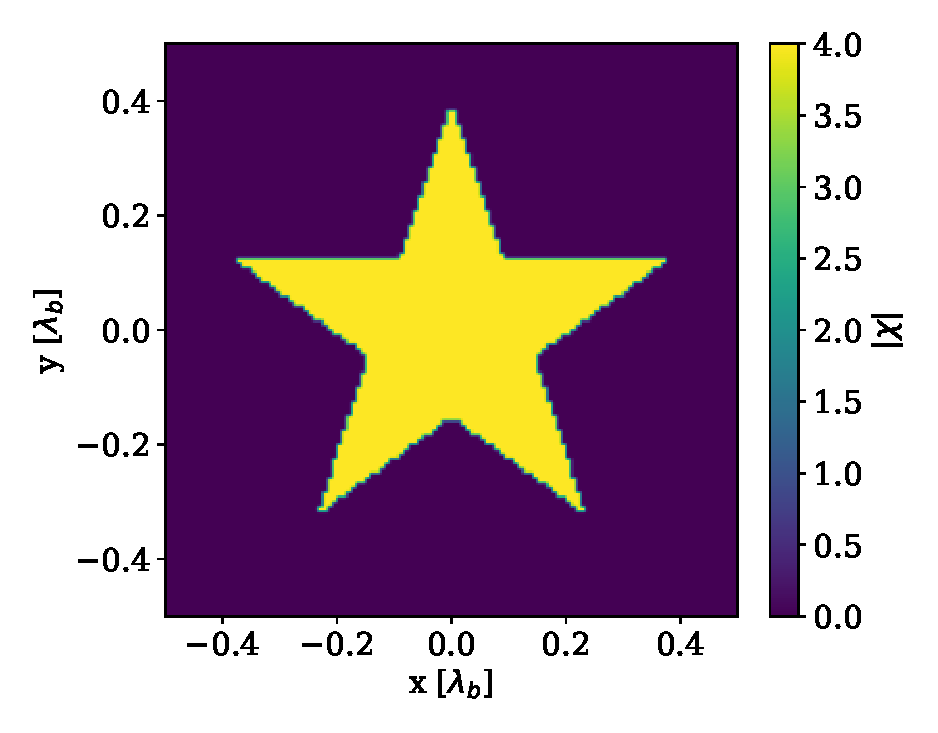
\includegraphics[width=.25\textwidth]{./figuras/casestudy/multiple/groundtruth}\label{fig:results:casestudy:multiple:reconstruction:groundtruth}}
				\subfloat[SAEA1]{\includegraphics[width=.25\textwidth]{./figuras/casestudy/multiple/reconstruction_saea1}\label{fig:results:casestudy:multiple:reconstruction:saea1}}
				\subfloat[SAEA2]{\includegraphics[width=.25\textwidth]{./figuras/casestudy/multiple/reconstruction_saea2}\label{fig:results:casestudy:multiple:reconstruction:saea2}}
				\subfloat[SAEA3]{\includegraphics[width=.25\textwidth]{./figuras/casestudy/multiple/reconstruction_saea3}\label{fig:results:casestudy:multiple:reconstruction:saea3}} \\
				\subfloat[SADM1]{\includegraphics[width=.25\textwidth]{./figuras/casestudy/multiple/reconstruction_sadm1}\label{fig:results:casestudy:multiple:reconstruction:sadm1}}
				\subfloat[SADM2]{\includegraphics[width=.25\textwidth]{./figuras/casestudy/multiple/reconstruction_sadm2}\label{fig:results:casestudy:multiple:reconstruction:sadm2}}
				\subfloat[EA]{\includegraphics[width=.25\textwidth]{./figuras/casestudy/multiple/reconstruction_ea}\label{fig:results:casestudy:multiple:reconstruction:ea}}
				\subfloat[BIM]{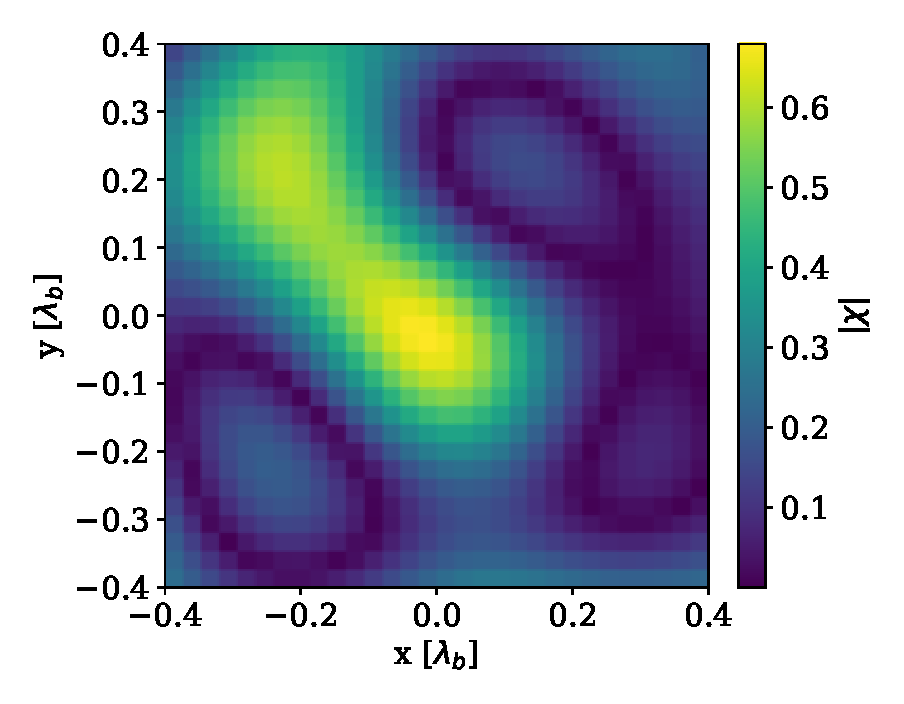
\includegraphics[width=.25\textwidth]{./figuras/casestudy/multiple/reconstruction_bim}\label{fig:results:casestudy:multiple:reconstruction:bim}} \\
				\subfloat[DBIM]{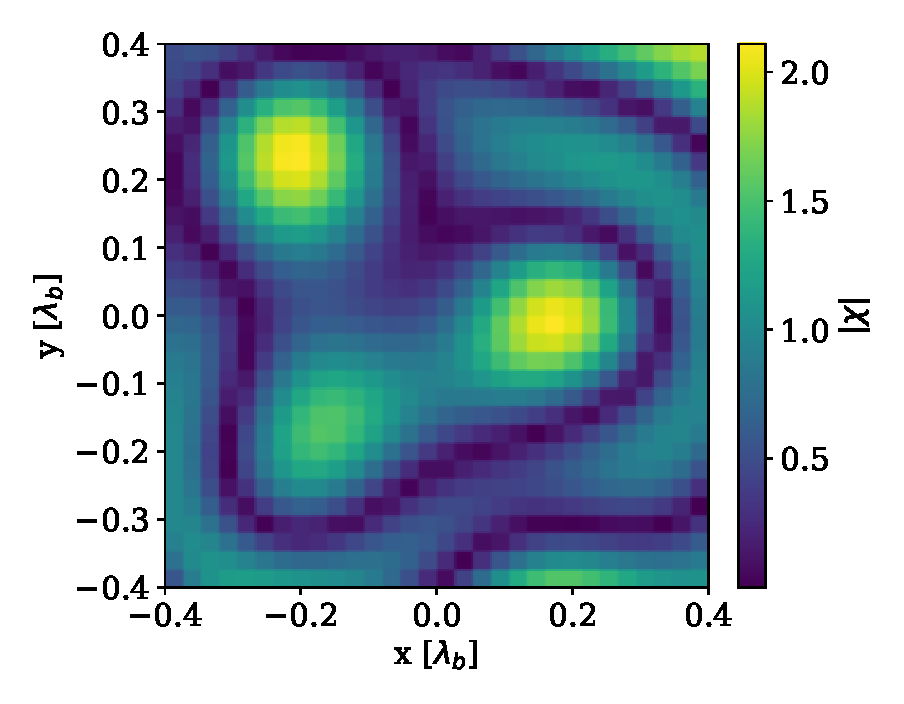
\includegraphics[width=.25\textwidth]{./figuras/casestudy/multiple/reconstruction_dbim}\label{fig:results:casestudy:multiple:reconstruction:dbim}}
				\subfloat[CGM]{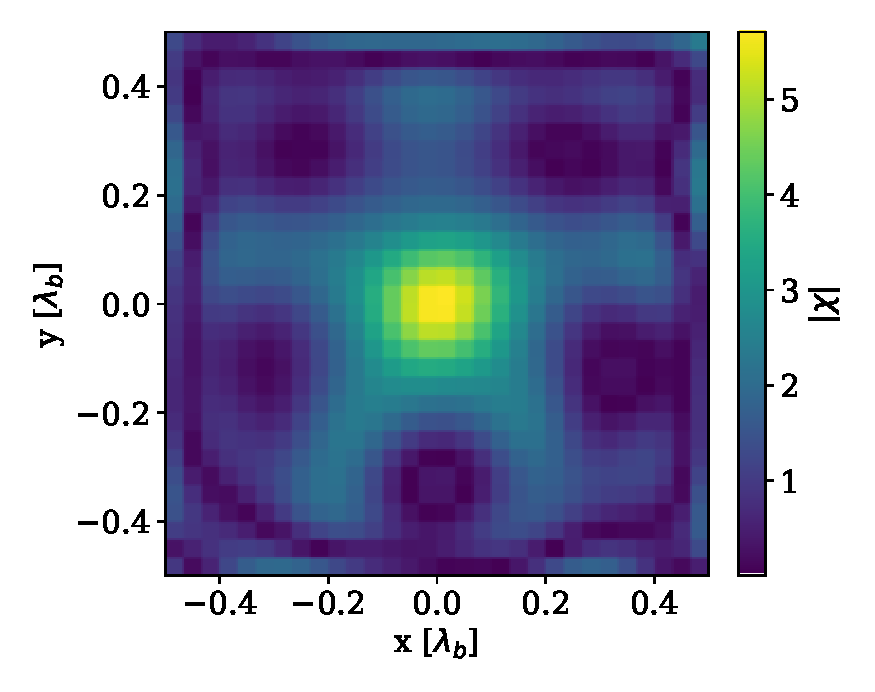
\includegraphics[width=.25\textwidth]{./figuras/casestudy/multiple/reconstruction_cgm}\label{fig:results:casestudy:multiple:reconstruction:cgm}}
				\subfloat[ECSI]{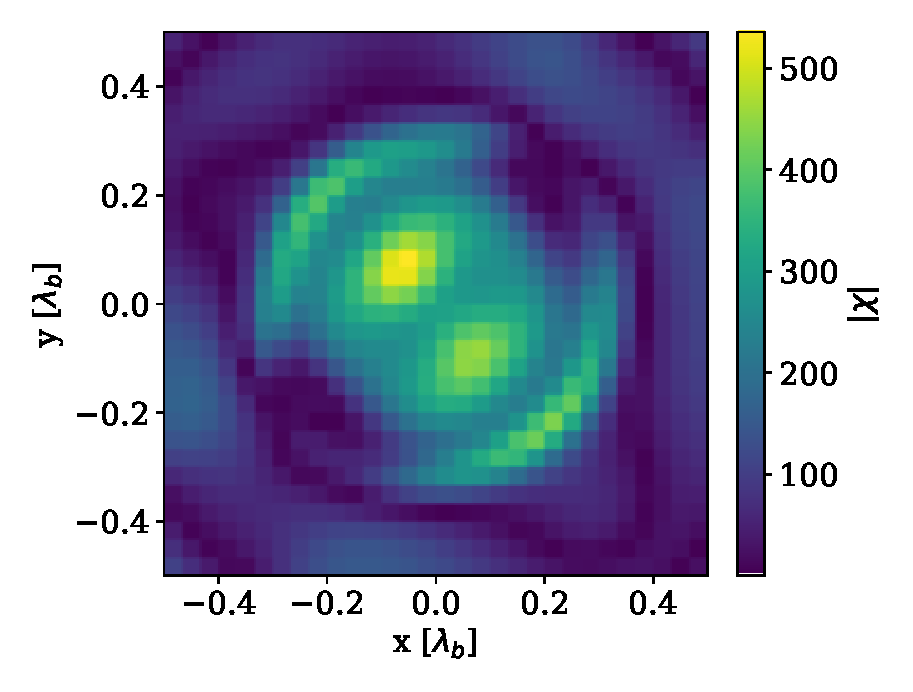
\includegraphics[width=.25\textwidth]{./figuras/casestudy/multiple/reconstruction_ecsi}\label{fig:results:casestudy:multiple:reconstruction:ecsi}}
				\subfloat[SOM]{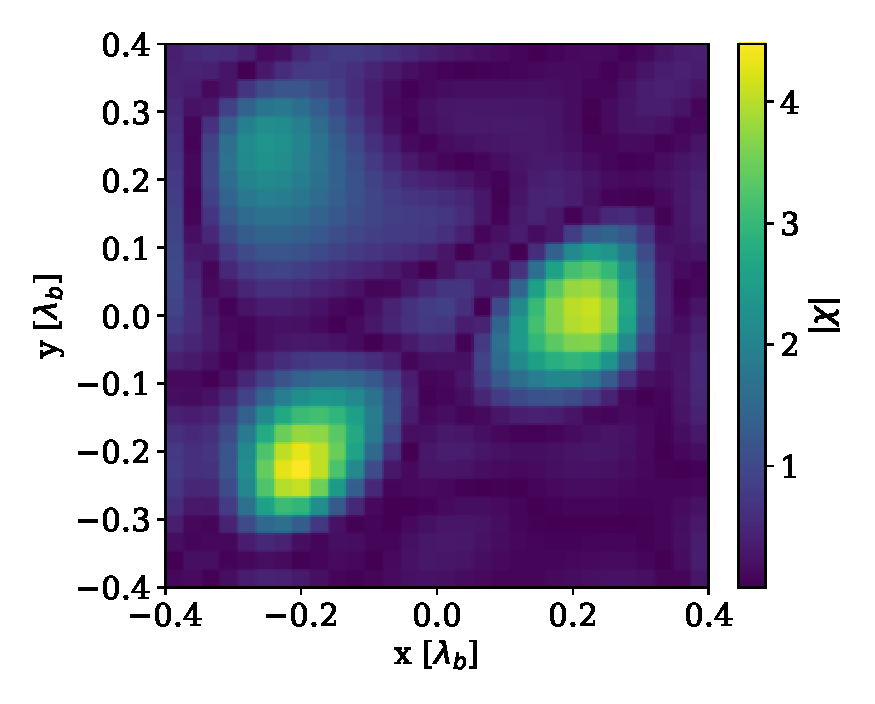
\includegraphics[width=.25\textwidth]{./figuras/casestudy/multiple/reconstruction_som}\label{fig:results:casestudy:multiple:reconstruction:som}} 
				\caption[Multiple scatterers case study: Comparison of image reconstructions using surrogate model-assisted algorithms and deterministic methods.]{Comparison of image reconstructions using surrogate model-assisted algorithms and deterministic methods considering the multiple scatterers case study: (a) shows the ground-truth image; (b), (c), and (d) depict the best image recovered by SAEA1, SAEA2, and SAEA3, respectively, in 30 execution according to $\zeta_{\epsilon OE}$ indicator; (e), (f) and (g) show the best image recovered by SADM1, SADM2, and EA, respectively, in 30 execution according to $\zeta_{\epsilon OE}$ indicator; (g) shows the image recovered by BIM, and (h) shows the image recovered by DBIM; finally, (i), (k), and (l) show the image recovered by CGM, ECSI, and SOM, respectively.}
				\label{fig:results:casestudy:multiple:reconstruction}
			\end{figure}
		
			% * A Fig. 5.7 apresenta as melhores reconstruções dos algoritmos que foram executados múltiplas vezes seguindo o mesmo critério do estudo de caso passado, assim como as imagens dos métodos determinísticos.
			% * No caso dos algoritmos baseados na transformação do problema, os espalhadores pareceram um pouco mais espaçados em relação ao centro da imagem reconstruída. Tanto é que os espalhadores ficaram muito próximos das bordas da imagem. Mas as melhores estimativas do contraste foram muito boas.
			% * O BIM não teve sucesso detectar os espalhadores.
			% * Na imagem do DBIM parece até haver três espalhadores. Porém, ainda há ondulações muito significativas na região de fundo.
			% * CGM, ECSI e SOM conseguiram fazer detecção de três espalhadores com valores bem próximos do exato. O CGM teve um pouco mais de dificuldade em relação às ondulações no meio de fundo.
			
			The results are presented in Fig. \ref{fig:results:casestudy:multiple:reconstruction}, which displays the best reconstructions of the algorithms that were executed multiple times following the same criteria as the previous case study, along with images of the deterministic methods. In the case of algorithms based on the transformation of the problem (Figs. \ref{fig:results:casestudy:multiple:reconstruction:saea1}-\ref{fig:results:casestudy:multiple:reconstruction:ea}), the scatterers appeared a little more displaced from the center of the reconstructed image, and they were very close to the edges of the image. However, the best estimates of the contrast were excellent. BIM (Fig. \ref{fig:results:casestudy:multiple:reconstruction:bim}) was not successful in detecting the scatterers, while DBIM (Fig. \ref{fig:results:casestudy:multiple:reconstruction:dbim}) displayed significant noise in the background region, even though it might look like there are three scatterers in the image. CGM, ECSI, and SOM (Figs. \ref{fig:results:casestudy:multiple:reconstruction:cgm}-\ref{fig:results:casestudy:multiple:reconstruction:som}) were able to detect three scatterers with values less close to the exact one than the proposed algorithms, although CGM had more difficulty with background noise.
		
			\begin{figure}[!h]
				\centering
				\subfloat[SAEA1]{\includegraphics[width=.25\textwidth]{./figuras/casestudy/multiple/convergence_saea1}\label{fig:results:casestudy:multiple:convergence:saea1}}
				\subfloat[SAEA2]{\includegraphics[width=.25\textwidth]{./figuras/casestudy/multiple/convergence_saea2}\label{fig:results:casestudy:multiple:convergence:saea2}}
				\subfloat[SAEA3]{\includegraphics[width=.25\textwidth]{./figuras/casestudy/multiple/convergence_saea3}\label{fig:results:casestudy:multiple:convergence:saea3}}
				\subfloat[SADM1]{\includegraphics[width=.25\textwidth]{./figuras/casestudy/multiple/convergence_sadm1}\label{fig:results:casestudy:multiple:convergence:sadm1}} \\
				\subfloat[SADM2]{\includegraphics[width=.25\textwidth]{./figuras/casestudy/multiple/convergence_sadm2}\label{fig:results:casestudy:multiple:convergence:sadm2}}
				\subfloat[EA]{\includegraphics[width=.25\textwidth]{./figuras/casestudy/multiple/convergence_ea}\label{fig:results:casestudy:multiple:convergence:ea}}
				\subfloat[BIM]{\includegraphics[width=.25\textwidth]{./figuras/casestudy/multiple/convergence_bim}\label{fig:results:casestudy:multiple:convergence:bim}}
				\subfloat[DBIM]{\includegraphics[width=.25\textwidth]{./figuras/casestudy/multiple/convergence_dbim}\label{fig:results:casestudy:multiple:convergence:dbim}} \\
				\subfloat[CGM]{\includegraphics[width=.25\textwidth]{./figuras/casestudy/multiple/convergence_cgm}\label{fig:results:casestudy:multiple:convergence:cgm}}
				\subfloat[ECSI]{\includegraphics[width=.25\textwidth]{./figuras/casestudy/multiple/convergence_ecsi}\label{fig:results:casestudy:multiple:convergence:ecsi}}
				\subfloat[SOM]{\includegraphics[width=.25\textwidth]{./figuras/casestudy/multiple/convergence_som}\label{fig:results:casestudy:multiple:convergence:som}} 
				\caption[Convergence of the objective function for the multiple scatterers case obtained by the stochastic and deterministic algorithms.]{Convergence of the objective function for the multiple scatterers case obtained by the stochastic and deterministic algorithms. (a) to (k) show the curves obtained by SAEA1, SAEA2, SAEA3, SADM1, SADM2, EA, BIM, DBIM, CGM, ECSI, and SOM algorithms, respectively. The x-axis represents the number of iterations, and the y-axis represents the value of the objective function of the correspondent algorithm.}
				\label{fig:results:casestudy:multiple:convergence}
			\end{figure}
		
			% * A Fig 5.8 mostra a convergência da função objetivo para cada um dos algoritmos.
			% * A convergência dos algoritmos SADM1 e SADM2 foi muito menos homogênea neste estudo de caso. Desta vez, o comportamento foi mais parecido com um algoritmo estocástico, como os SAEAs. Embora as decisões dentro do processo iterativo dos SADMs seja determinísticas, a hipótese é que os processos dentro do treinamento do modelo substituto sejam a causa para as diferenças nas curvas de convergência entre as execuções. E isso se torna mais acentuado em cenários de espalhadores com alto contraste.
			% * As curvas de convergência dos algoritmos SAEAs foram semelhantes às do estudo de caso passado. Nota-se que o SAEA1 tende a ter curvas um pouco mais homogêneas do que o SAEA3 e que, embora o SAEA2 tenha tido apenas 3 gerações, algumas das execuções encontraram soluções com o mesmo valor da função objetivo que as melhores soluções encontradas pelos os outros dois algoritmos.
			% * A convergência dos algoritmos CGM, ECSI e SOM mostram que eles terminaram suas execuções com soluções estáveis. Logo, mesmo se mais iterações fossem dadas, as imagens reconstruídas não iriam diferir significativamente daquelas mostradas nas Figs. 5.7 (j)-(l). Logo, nesta instância, esses algoritmos não iriam conseguir uma reconstrução melhor.
			
			Figure \ref{fig:results:casestudy:multiple:convergence} presents the convergence of the objective function for each algorithm. Interestingly, the convergence of the SADM1 and SADM2 algorithms (Figs. \ref{fig:results:casestudy:multiple:convergence:sadm1}-\ref{fig:results:casestudy:multiple:convergence:sadm2}) was less homogeneous in this case study, behaving more like a stochastic algorithm such as SAEAs. Although the decisions within the iterative process of SADMs are deterministic, the differences in the convergence curves between runs could be due to the processes within the surrogate model training, which can be more complex in high-contrast scattering scenarios.
			
			On the other hand, the convergence curves of the SAEAs algorithms were similar to those of the previous case study. SAEA1 (Fig. \ref{fig:results:casestudy:multiple:convergence:saea1}) had slightly more homogeneous curves than SAEA3 (Fig. \ref{fig:results:casestudy:multiple:convergence:saea3}), and even though SAEA2 (Fig. \ref{fig:results:casestudy:multiple:convergence:saea2}) had only 3 generations, some of the runs found solutions with the same objective function value as the best solutions found by the other two algorithms.
			
			Finally, the convergence of the CGM, ECSI, and SOM algorithms (Figs. \ref{fig:results:casestudy:multiple:convergence:cgm}-\ref{fig:results:casestudy:multiple:convergence:som}) indicates that they finished their runs with stable solutions. Therefore, even if more iterations were given, the reconstructed images would not significantly differ from those shown in Figures \ref{fig:results:casestudy:multiple:reconstruction:cgm}-\ref{fig:results:casestudy:multiple:reconstruction:som}. In this scenario, these algorithms would not obtain a better reconstruction.
		
			\begin{figure}
				\centering
				\includegraphics[width=.9\textwidth]{./figuras/casestudy/multiple/boxplot_zeta_eoe}
				\caption[Performance of $\zeta_{\epsilon OE}$ indicator for various algorithms in the multiple scatterers case study.]{Performance of $\zeta_{\epsilon OE}$ indicator for various algorithms in the multiple scatterers case study. Boxplots show quartiles of 30 executions for stochastic algorithms, and the solid line represents the deterministic algorithms.}
				\label{fig:results:casestudy:multiple:boxplot:zeta_eoe}
			\end{figure}
		
			% * A Fig. 5.9 apresenta os resultados do indicador $\zeta_{\epsilon OE}$ para cada algoritmo.
			% * O CGM foi o algoritmo com menor erro na estimativa do contraste dos objetos, embora a imagem reconstruída como um todo não tenha sido tão boa (Fig. \ref{fig:results:casestudy:multiple:reconstruction:cgm}). Mesmo superestimando o contraste ligeiramente mais que os algoritmos assistidos por modelos substitutos, o erro pode ter sido menor por não exibir o comportamento de afastamento, o que acaba influenciando muito na medida do erro.
			% * Embora a posição da mediana do algoritmo SAEA1 esteja acima das demais dos outros algoritmos assistidos por modelos substitutos, o Kruskal-Wallis H-Test não detecta diferenças na mediana da performance entre todos esses algoritmos (p-valor = 0.655). Logo, não é possível afirmar que alguns desses algoritmos teve uma performance mediana melhor.
			% * Embora as medianas dos algoritmos assistidos por modelos substitutos estejam acima dos valores encontrados pelos métodos SOM, CGM e ECSI, a diferença não chega a ser mais que 20 [\%/pixel].
		
			In Figure \ref{fig:results:casestudy:multiple:boxplot:zeta_eoe}, the results of indicator $\zeta_{\epsilon OE}$ for each algorithm are presented. The CGM algorithm had the lowest error in estimating the contrast of objects, but its reconstructed image was not as satisfactory as the other algorithms (Fig. \ref{fig:results:casestudy:multiple:reconstruction:cgm}). However, even with a slight overestimation of the contrast compared to the surrogate model-assisted algorithms, the error may have been smaller due to the lack of distancing behavior observed for the proposed algorithm and that influences the error measure. The Kruskal-Wallis H-Test did not detect any differences in the median performance between the surrogate model-assisted algorithms, despite SAEA1 having a higher median position. The algorithms assisted by surrogate models had higher medians than the SOM, CGM, and ECSI methods, but the difference did not exceed 20 [\%/pixel].
		
			\begin{figure}
				\centering
				\includegraphics[width=.9\textwidth]{./figuras/casestudy/multiple/boxplot_zeta_s}
				\caption[Performance of shape error estimation quantified by the $\zeta_S$ indicator obtained by the set of algorithms considering the multiple scatterers case study.]{Performance of shape error estimation quantified by the $\zeta_S$ indicator obtained by the set of algorithms considering the multiple scatterers case study. The boxes represent the quartiles of the 30 executions of the stochastic algorithms, while the other points indicate the obtained values by the deterministic ones. The shape error is calculated based on the ground-truth image and the reconstructed image obtained by each algorithm.}
				\label{fig:results:casestudy:multiple:boxplot:zeta_s}
			\end{figure}
			
			% * A Fig. 5.10 apresenta os resultados do indicador X que quantifica a recuperação de forma dos espalhadores pelos algoritmos.
			% * Da mesma maneira como no indicador de erro de estimativa de contraste, o CGM teve o menor erro de recuperação de forma. No entanto, dessa vez, a diferença foi mais significativa chegando a, aproximadamente, 50 [\%] de diferença entre o segundo algoritmo. Ainda assim, vale lembrar que nenhum algoritmo conseguiu reconstruir formas que efetivamente se parecessem com os espalhadores, conforme mostrado na Fig. \ref{fig:results:casestudy:multiple:reconstruction}.
			% * A mediana dos algoritmos assistidos por modelo substituto são bem próximas. No entanto, se compararmos as medianas dos algoritmos SAEA2, SAEA3, SADM1 e SADM2, nenhuma diferença será detectada pelo Kruskal-Wallis H-Test a um nível de significância de 5\% (valor-p = 0.065). No entanto, quando adicionamos o SAEA1 nessa comparação, a performance mediana desse algoritmo será melhor que a dos outros algoritmos (valor-p $<0.001$ em todas as comparações post-hoc). Portanto, o SAEA1 teve uma performance mediana melhor, mas a diferença também não é tão grande e significativa do ponto de vista da imagem reconstruída.
			
			The results of the $\zeta_S$ indicator that evaluates the shape recovery of the scatterers by the algorithms is presented in Fig. \ref{fig:results:casestudy:multiple:boxplot:zeta_s}. The CGM algorithm had the lowest shape recovery error, with a significant difference of around 50 [\%] compared to the second-best algorithm. However, none of the algorithms were able to reconstruct shapes that resembled the scatterers.
			
			Regarding the surrogate model-assisted algorithms, the medians were very close to each other. When comparing the medians of SAEA2, SAEA3, SADM1, and SADM2 algorithms, the Kruskal-Wallis H-Test did not detect any difference at a significance level of 5\% (p-value $= 0.065$). However, when including SAEA1 in the comparison, it showed a better median performance than the other algorithms (p-value $< 0.001$ in all post-hoc comparisons). Nonetheless, the difference is not significant enough from the point of view of the reconstructed image.
			
			\begin{figure}
				\centering
				\includegraphics[width=.9\textwidth]{./figuras/casestudy/multiple/boxplot_time}
				\caption[Box plot showing the execution time distribution of the set of algorithms considered for the multiple scatterers case study.]{Box plot showing the execution time distribution of the set of algorithms considered for the multiple scatterers case study. The boxes represent the quartiles of the 30 executions of the stochastic algorithms, and the whiskers represent the minimum and maximum values. The deterministic algorithms are represented by individual points. The execution time results are presented in seconds.}
				\label{fig:results:casestudy:multiple:boxplot:time}
			\end{figure}
		
			% * A Fig. 5.11 apresenta os resultados do tempo de execução dos algoritmos.
			% * O tempo de execução do BIM e do DBIM foi menor tendo em vista que poucas iterações foram necessárias, e assim, o cálculo mais custoso foi menos vezes acionado durante a execução do algoritmo.
			% * A performance mediana dos algoritmos SADM2 e EA foram muito semelhantes, de modo que não foi detectada diferença segundo o Welch Two Sample T-Test (valor-p = 0.203). No entanto, a mediana destes dois estão abaixo dos demais algoritmos.
			% * Levando em consideração este indicador junto com os indicadores $\zeta_{\epsilon OE}$ e $\zeta_S$, a escolha entre SADM2 e o CGM nesta instância pode ser entendida como uma troca entre qualidade da reconstrução e tempo de execução. Em outras palavras, o SADM2 pode não alcançar a mesma performance que o CGM nos indicadores de forma e estimativa de contraste, mas consegue alcançar valores não tão maiores por um tempo bem menor.
			
			Figure \ref{fig:results:casestudy:multiple:boxplot:time} displays the results of the execution time of the algorithms. BIM and DBIM had shorter execution times since fewer iterations were needed, which means the most expensive calculation was called fewer times during the algorithm execution. The median performances of the SADM2 and EA algorithms were quite similar, and no significant difference was detected based on the Welch Two Sample T-Test (p-value = 0.203). However, the medians of these two algorithms were below that of the other algorithms. By considering this indicator along with the $\zeta_{\epsilon OE}$ and $\zeta_S$ indicators, choosing between SADM2 and CGM in this case could be seen as a trade-off between reconstruction quality and execution time. In other words, while SADM2 may not achieve the same performance as CGM in shape and contrast estimation indicators, it can achieve slightly higher values in a much shorter time.
		
			\begin{figure}
				\centering
				\subfloat[]{\includegraphics[width=.45\textwidth]{./figuras/casestudy/multiple/surface1}\label{fig:results:casestudy:multiple:boxplot:surface:1}} \hspace{.05\textwidth}
				\subfloat[]{\includegraphics[width=.45\textwidth]{./figuras/casestudy/multiple/surface2}\label{fig:results:casestudy:multiple:boxplot:surface:2}}
				\caption[Surface of the two-dimensional optimization problem obtained from the transformation of the multiple scatterers case study and the final solutions obtained by different algorithms.]{Surface of the two-dimensional optimization problem obtained from the transformation of the multiple scatterers case study and the final solutions obtained by different algorithms. Subfigure (a) shows the final solutions obtained by SAEA1, SAEA2, and SADM1 algorithms, while subfigure (b) shows the final solutions obtained by EA, SAEA3, and SADM2 algorithms.}
				\label{fig:results:casestudy:multiple:surface}
			\end{figure}
		
			% * A Fig. 5.12 exibe a superfície da função objetivo resultante da transformação em um problema de otimização bidimensional e a localização das soluções finais encontradas pelos algoritmos nas múltiplas execuções.
			% * Com o aumento da não-linearidade do problema, a superfície ficou menos convexa.
			% * Além disso, a imagem também mostra um certo agrupamento de soluções em torno do ponto ($T$, $\chi$) $=$ (0.75, 4) e outro menor em torno de (0.8, 5). Pode ser que este último seja um mínimo local onde algumas das execuções poderiam ter ficado presas. A ocorrência de mínimos locais mais difíceis de escapar pode ser mais comum a medida que o problema vai ficando mais não-linear ou o contraste dos espalhadores vai subindo.
			% * As soluções finais encontradas de todos algoritmos ficaram espalhadas sendo que apenas no caso do EA é que houveram soluções fora da região de subnível mais baixa.
		
			Figure \ref{fig:results:casestudy:multiple:surface} presents the surface of the objective function resulting from the transformation in a two-dimensional optimization problem, along with the location of the final solutions found by the algorithms in multiple runs. As the nonlinearity of the problem increased, the surface became less convex, and there was a certain grouping of solutions around the point $T$, $\chi$) $=$ (0.75, 4) and a smaller one around (0.8, 5). It is possible that the latter is a local minimum where some of the runs may have gotten stuck. The occurrence of more difficult to escape local minima may be more common as the problem becomes more non-linear or the contrast of the scatterers increases. The final solutions found for all algorithms were scattered, and only in the case of EA that solutions outside the lowest sublevel region were returned.
		
		\subsection{Non-Homogeneous Scatterer}\label{chap:results:casestudy:nonhomogeneous}
		
			% * The thrid case study considers a nonhomogeneous scatterer.
			% * This scenario is relevant since OSM is qualitative method that allows to identify different levels of contrast.
			% * The case study is inspired in an experiment presented in \citep{bevacqua2021effective}.
			% * The scatterer is a square which side is $\lambda_b$. Within the square, there are three regions where the contrast is 0.4, 0.9, and 1.25.
			% * Further information regarding the scatterer specification can be found in the mentioned reference.
			% * The Table 3 shows the specifications for measurement and imaging domains.
			% * The Degree of Non-Linearity for this case is 1.396, which is above the threshold for cases that the Born Approximation may be applied.
			% * The scatterer is illustrated in Figure 5.13 (a).
			% * All settings for synthesizing the scattered field data are the same as in the previous case study.
			
			The third case study presented in this work focuses on the imaging of a nonhomogeneous scatterer, which is a square of side length equals to $\lambda_b$ with three different regions of contrast (0.4, 0.9, and 1.25) inside it. This scenario is relevant because it allows the qualitative identification of different levels of contrast using the OSM method. The inspiration for this study comes from a similar experiment presented by \cite{bevacqua2020physical}. The scatterer's detailed specifications can be found in the reference. Table \ref{tab:results:casestudy:nonhomogeneous:configuration} provides the specifications for measurement and imaging domains. Figure \ref{fig:results:casestudy:nonhomogeneous:reconstruction:groundtruth} illustrates the scatterer. The degree of non-linearity for this case is 1.396, which is above the threshold for cases where the Born Approximation can be applied. All settings for synthesizing the scattered field data are the same as in the previous case study.
			
			\begin{table}[!h]
				\centering
				\caption[Parameters for the nonhomogeneous scatterer case study.]{Parameters for problem specification of the nonhomogeneous scatterer case study.}
				\rowcolors{1}{gray2}{gray1}
				\begin{tabular}{cccccc}
					$N_M$ & $N_S$ & $\lambda_b$ & $R_O$ & $L_X$, $L_Y$ & $\epsilon_{rb}$ \\
					16 & 16 & 1 [m] & 3.33 [$\lambda_b$] & 1.67 [$\lambda_b$] & 1
				\end{tabular}
				\label{tab:results:casestudy:nonhomogeneous:configuration}
			\end{table}
			
			For this case study, adjustments were made to the algorithm configurations to more effectively explore their behavior. For the problem transformation-based algorithms, the maximum limit for the contrast variable was reduced to 3 since the maximum contrast in the true image is now 1.25. The stopping criterion was set to 60 evaluations. SAEA2 and EA utilized populations of 20 individuals as in the previous case study. Deterministic methods also underwent some modifications, such as CGM and ECSI using 50 iterations, DBIM using 3 iterations, BIM using 15 iterations, and SOM using 500 iterations with a cut-off index of 5.
		
			\begin{figure}[!h]
				\centering
				\subfloat[Ground-Truth]{\includegraphics[width=.25\textwidth]{./figuras/casestudy/nonhomogeneous/groundtruth}\label{fig:results:casestudy:nonhomogeneous:reconstruction:groundtruth}}
				\subfloat[SAEA1]{\includegraphics[width=.25\textwidth]{./figuras/casestudy/nonhomogeneous/reconstruction_saea1}\label{fig:results:casestudy:nonhomogeneous:reconstruction:saea1}}
				\subfloat[SAEA2]{\includegraphics[width=.25\textwidth]{./figuras/casestudy/nonhomogeneous/reconstruction_saea2}\label{fig:results:casestudy:nonhomogeneous:reconstruction:saea2}}
				\subfloat[SAEA3]{\includegraphics[width=.25\textwidth]{./figuras/casestudy/nonhomogeneous/reconstruction_saea3}\label{fig:results:casestudy:nonhomogeneous:reconstruction:saea3}} \\
				\subfloat[SADM1]{\includegraphics[width=.25\textwidth]{./figuras/casestudy/nonhomogeneous/reconstruction_sadm1}\label{fig:results:casestudy:nonhomogeneous:reconstruction:sadm1}}
				\subfloat[SADM2]{\includegraphics[width=.25\textwidth]{./figuras/casestudy/nonhomogeneous/reconstruction_sadm2}\label{fig:results:casestudy:nonhomogeneous:reconstruction:sadm2}}
				\subfloat[EA]{\includegraphics[width=.25\textwidth]{./figuras/casestudy/nonhomogeneous/reconstruction_ea}\label{fig:results:casestudy:nonhomogeneous:reconstruction:ea}}
				\subfloat[BIM]{\includegraphics[width=.25\textwidth]{./figuras/casestudy/nonhomogeneous/reconstruction_bim}\label{fig:results:casestudy:nonhomogeneous:reconstruction:bim}} \\
				\subfloat[DBIM]{\includegraphics[width=.25\textwidth]{./figuras/casestudy/nonhomogeneous/reconstruction_dbim}\label{fig:results:casestudy:nonhomogeneous:reconstruction:dbim}}
				\subfloat[CGM]{\includegraphics[width=.25\textwidth]{./figuras/casestudy/nonhomogeneous/reconstruction_cgm}\label{fig:results:casestudy:nonhomogeneous:reconstruction:cgm}}
				\subfloat[ECSI]{\includegraphics[width=.25\textwidth]{./figuras/casestudy/nonhomogeneous/reconstruction_ecsi}\label{fig:results:casestudy:nonhomogeneous:reconstruction:ecsi}}
				\subfloat[SOM]{\includegraphics[width=.25\textwidth]{./figuras/casestudy/nonhomogeneous/reconstruction_som}\label{fig:results:casestudy:nonhomogeneous:reconstruction:som}} 
				\caption[Nonhomogeneous scatterer case study: Comparison of image reconstructions using surrogate model-assisted algorithms and deterministic methods.]{Comparison of image reconstructions using surrogate model-assisted algorithms and deterministic methods considering the nonhomogeneous scatterer case study: (a) shows the ground-truth image; (b), (c), and (d) depict the best image recovered by SAEA1, SAEA2, and SAEA3, respectively, in 30 execution according to $\zeta_{\epsilon OE}$ indicator; (e), (f) and (g) show the best image recovered by SADM1, SADM2, and EA, respectively, in 30 execution according to $\zeta_{\epsilon OE}$ indicator; (g) shows the image recovered by BIM, and (h) shows the image recovered by DBIM; finally, (i), (k), and (l) show the image recovered by CGM, ECSI, and SOM, respectively.}
				\label{fig:results:casestudy:nonhomogeneous:reconstruction}
			\end{figure}
		
			% * A Fig. 5.13 apresenta as melhores reconstruções dos algoritmos que foram executados múltiplas vezes seguindo o mesmo critério do estudo de caso passado, assim como as imagens dos métodos determinísticos.
			% * As imagens reconstruídas pelos algoritmos propostos são bem semelhantes entre si, i.e., parecem ser reconstruídas a partir do mesmo nível de limiar e de estimativa de contraste. O nível mais baixo de contraste do espalhador parece estar proporcionalmente mais alto do que na imagem original, que modo que este nível se confunde um pouco com o segundo. Isto tem a ver com a performance do método qualitativo neste tipo de cenário, i.e., o OSM pode ter uma certa dificuldade de estimar bem as diferenças quando essas começam a ficar distante uma das outras. Possivelmente por causa disso é que o contraste ficou subestimado em todos os resultados, uma vez que o erro da equação de dados poderia crescer muito se a média de contraste no espalhador subisse para que o máximo valor alcançasse o valor verdadeiro.
			% * O BIM fez uma boa reconstrução. No resultado obtido por ele, o contorno do espalhador ficou levemente destacado e os níveis de contraste bem estimados. Já o DBIM não teve uma resultado tão bom assim.
			% * CGM e ECSI até realizaram reconstruções cujo o formato do espalhador até se assemelha ao verdadeiro. No entanto, no CGM, o contraste foi superestimado e, no ECSI, a região de contraste mais alto ficou um pouco distorcida.
			% * O SOM não realizou uma boa reconstrução. Possivelmente porque o nível de ruído pode ter afetado muito o desempenho do método nesse tipo de cenário.
			
			Figure \ref{fig:results:casestudy:nonhomogeneous:reconstruction} presents the best reconstructions of the algorithms executed multiple times under the same criteria as the previous case study, as well as the images of the deterministic methods. The reconstructed images by the proposed algorithms (Figs. \ref{fig:results:casestudy:nonhomogeneous:reconstruction:saea1}-\ref{fig:results:casestudy:nonhomogeneous:reconstruction:ea}) were very similar to each other, suggesting that they were reconstructed from the same threshold level and contrast estimation. However, the lowest level of contrast in the scatterer appeared to be proportionately higher than in the original image, resulting in a relatively blurred image with the second level. This may be attributed to the difficulty of the OSM method in estimating differences when they become distant from each other. As a result, the contrast was underestimated in all results since the increment in the contrast multiplication factor would represent an object with a higher average contrast and a higher erro in the data equation.
			
			BIM had a satisfactory reconstruction with a notable contour of the scatterer and well-estimated contrast levels. On the other hand, DBIM did not perform well. CGM and ECSI performed reconstructions that resembled the real scatterer, but with some distortions. In CGM, the contrast was overestimated, and in ECSI, the highest contrast region was slightly distorted. Finally, SOM did not perform well, possibly because the noise level greatly affected its performance in this scenario.
		
			\begin{figure}[!h]
				\centering
				\subfloat[SAEA1]{\includegraphics[width=.25\textwidth]{./figuras/casestudy/nonhomogeneous/convergence_saea1}\label{fig:results:casestudy:nonhomogeneous:convergence:saea1}}
				\subfloat[SAEA2]{\includegraphics[width=.25\textwidth]{./figuras/casestudy/nonhomogeneous/convergence_saea2}\label{fig:results:casestudy:nonhomogeneous:convergence:saea2}}
				\subfloat[SAEA3]{\includegraphics[width=.25\textwidth]{./figuras/casestudy/nonhomogeneous/convergence_saea3}\label{fig:results:casestudy:nonhomogeneous:convergence:saea3}}
				\subfloat[SADM1]{\includegraphics[width=.25\textwidth]{./figuras/casestudy/nonhomogeneous/convergence_sadm1}\label{fig:results:casestudy:nonhomogeneous:convergence:sadm1}} \\
				\subfloat[SADM2]{\includegraphics[width=.25\textwidth]{./figuras/casestudy/nonhomogeneous/convergence_sadm2}\label{fig:results:casestudy:nonhomogeneous:convergence:sadm2}}
				\subfloat[EA]{\includegraphics[width=.25\textwidth]{./figuras/casestudy/nonhomogeneous/convergence_ea}\label{fig:results:casestudy:nonhomogeneous:convergence:ea}}
				\subfloat[BIM]{\includegraphics[width=.25\textwidth]{./figuras/casestudy/nonhomogeneous/convergence_bim}\label{fig:results:casestudy:nonhomogeneous:convergence:bim}}
				\subfloat[DBIM]{\includegraphics[width=.25\textwidth]{./figuras/casestudy/nonhomogeneous/convergence_dbim}\label{fig:results:casestudy:nonhomogeneous:convergence:dbim}} \\
				\subfloat[CGM]{\includegraphics[width=.25\textwidth]{./figuras/casestudy/nonhomogeneous/convergence_cgm}\label{fig:results:casestudy:nonhomogeneous:convergence:cgm}}
				\subfloat[ECSI]{\includegraphics[width=.25\textwidth]{./figuras/casestudy/nonhomogeneous/convergence_ecsi}\label{fig:results:casestudy:nonhomogeneous:convergence:ecsi}}
				\subfloat[SOM]{\includegraphics[width=.25\textwidth]{./figuras/casestudy/nonhomogeneous/convergence_som}\label{fig:results:casestudy:nonhomogeneous:convergence:som}} 
				\caption[Convergence of the objective function for the nonhomogeneous scatterer case obtained by the stochastic and deterministic algorithms.]{Convergence of the objective function for the nonhomogeneous scatterer case obtained by the stochastic and deterministic algorithms. (a) to (k) show the curves obtained by SAEA1, SAEA2, SAEA3, SADM1, SADM2, EA, BIM, DBIM, CGM, ECSI, and SOM algorithms, respectively. The x-axis represents the number of iterations, and the y-axis represents the value of the objective function of the correspondent algorithm.}
				\label{fig:results:casestudy:nonhomogeneous:convergence}
			\end{figure}
		
			% * A Fig. 5.14 mostra as curvas de convergência da função objetivo para os algoritmos considerados.
			% * Os algoritmos SADM1 e SADM2 tiveram leves variações entre as execuções.
			% * Embora o SAEA2 tenha tido 3 gerações, algumas das execuções conseguiram a chegar em soluções com valores de função objetivo baixos como as soluções finais de SAEA1 e SAEA3.
			% * BIM, CGM, ECSI e SOM terminaram suas execuções após alcançarem um nível razoável de estabilidade no processo de convergência. Portanto, mais iterações não iriam mudar muito em a qualidade das imagens reconstruídas.
			
			Figure \ref{fig:results:casestudy:nonhomogeneous:convergence} presents the convergence curves of the considered algorithms in this study. The figure shows that BIM, CGM, ECSI, and SOM reached a reasonable level of stability in the convergence process and ended their executions, indicating that further iterations would not significantly improve the quality of the reconstructed images. Meanwhile, SADM1 and SADM2 had slight variations between runs, and although SAEA2 had 3 generations, some of the runs were able to arrive at solutions with low objective function values like the final solutions of SAEA1 and SAEA3.
		
			\begin{figure}
				\centering
				\includegraphics[width=.9\textwidth]{./figuras/casestudy/nonhomogeneous/boxplot_zeta_eoe}
				\caption[Performance of $\zeta_{\epsilon OE}$ indicator for various algorithms in the nonhomogeneous scatterer case study.]{Performance of $\zeta_{\epsilon OE}$ indicator for various algorithms in the nonhomogeneous scatterer case study. Boxplots show quartiles of 30 executions for stochastic algorithms, and the solid line represents the deterministic algorithms.}
				\label{fig:results:casestudy:nonhomogeneous:boxplot:zeta_eoe}
			\end{figure}
		
			% * A Figura 5.15 mostra os resultados do indicador X obtidos pelos algoritmos.
			% * Embora a imagem reconstruída pelo BIM tenha sido a mais satisfatória, o menor erro de estimativa de contraste foi obtido pelo ECSI. Embora a forma tenha ficado um pouco distorcida, a estimativa em cada píxel pelo ECSI foi melhor.
			% * As medianas da performance dos algoritmos propostos foram bem similares e o Kruskal-Wallis H-Test falha em rejeitar a hipótese de igualdade entre elas (valor-p = 0.08). A diferença entre a performance deles e o ECSI foi, aproximadamente, 3 [%/pixel], o que não é tão ruim.
			
			The performance of the algorithms regarding the contrast estimation in the scatterer area was analyzed based on the results of indicator $\zeta_{\epsilon OE}$ presented in Figure \ref{fig:results:casestudy:nonhomogeneous:boxplot:zeta_eoe}. Despite the fact that the image reconstructed by BIM was the most satisfactory, with a well-estimated contrast and reasonably clear scatterer contour, ECSI was the algorithm with the lowest contrast estimation error, although the shape was slightly distorted. Nevertheless, the difference in performance between BIM and ECSI was not significant, with approximately 1 [\%/pixel]. The performance medians of the proposed algorithms were very similar, and the Kruskal-Wallis H-Test failed to reject the hypothesis of equality between them (p-value $= 0.08$). The performance difference between the proposed algorithms and ECSI was not too large, at around 3 [\%/pixel].
		
			\begin{figure}
				\centering
				\includegraphics[width=.9\textwidth]{./figuras/casestudy/nonhomogeneous/boxplot_zeta_s}
				\caption[Performance of shape error estimation quantified by the $\zeta_S$ indicator obtained by the set of algorithms considering the nonhomogeneous scatterer case study.]{Performance of shape error estimation quantified by the $\zeta_S$ indicator obtained by the set of algorithms considering the nonhomogeneous scatterer study. The boxes represent the quartiles of the 30 executions of the stochastic algorithms, while the other points indicate the obtained values by the deterministic ones. The shape error is calculated based on the ground-truth image and the reconstructed image obtained by each algorithm.}
				\label{fig:results:casestudy:nonhomogeneous:boxplot:zeta_s}
			\end{figure}
		
			% * A Figura 5.15 mostra os resultados do indicador X obtidos pelos algoritmos.
			% * Os algoritmos propostos tiveram uma performance melhor que os métodos determinísticos.
			% * O desempenho ruim do BIM neste indicador pode estar relacionado à dificuldade da aplicação do indicador em imagens muito heterogêneas. Para os algoritmos propostos, este indicador pode ter sido mais baixo por causa da menor heterogeneidade do espalhador e diferença em relação ao meio de fundo.
			% * Entre os algoritmos assistidos por modelos substituto, não há evidências para diferença na performance mediana do indicador, conforme o Kruskal-Wallis H-Test (valor-p = 0.088).
			
			Figure \ref{fig:results:casestudy:nonhomogeneous:boxplot:zeta_s} shows the results obtained by the algorithms considering the $\zeta_S$ indicator. It was observed that the proposed algorithms outperformed the deterministic methods in terms of this indicator. However, it is interesting to note that BIM performed relatively worse than the other proposed algorithms, and this may be related to the difficulty of applying the indicator to significantly heterogeneous images. On the other hand, the proposed algorithms performed better possibly due to the smaller heterogeneity of the scatterer and the difference in respect to the background medium. Among the surrogate model-assisted algorithms, there was no evidence of a significant difference in the median performance of the indicator, as confirmed by the Kruskal-Wallis H-Test (p-value $= 0.088$). This suggests that the performance of the proposed algorithms in terms of this indicator is similar, and none of them stands out significantly from the others.
		
			\begin{figure}
				\centering
				\includegraphics[width=.9\textwidth]{./figuras/casestudy/nonhomogeneous/boxplot_time}
				\caption[Box plot showing the execution time distribution of the set of algorithms considered for the nonhomogeneous scatterer case study.]{Box plot showing the execution time distribution of the set of algorithms considered for the nonhomogeneous scatterer case study. The boxes represent the quartiles of the 30 executions of the stochastic algorithms, and the whiskers represent the minimum and maximum values. The deterministic algorithms are represented by individual points. The execution time results are presented in seconds.}
				\label{fig:results:casestudy:nonhomogeneous:boxplot:time}
			\end{figure}
		
			% * A Figura 5.17 mostra os resultados para o tempo de execução dos algoritmos.
			% * O DBIM teve o menor tempo, uma vez que o número de iterações foi bem baixo.
			% * Em seguida, o BIM obteve o segundo menor tempo. Logo, o BIM consegue em um tempo razoavelmente pequeno, reconstruir a imagem adequadamente.
			% * Alguns dos algoritmos propostos (SAEA2, SADM1, SADM2 e EA) tiveram tempos de execução menor que algoritmos com o SOM e o CGM.
			
			Figure \ref{fig:results:casestudy:nonhomogeneous:boxplot:time} displays the running time of the algorithms analyzed in the study. As expected, some of the deterministic methods required less computational time than the proposed algorithms that use surrogate models. Among them, DBIM had the shortest time, thanks to the low number of iterations in which it can run without diverging. The second shortest time was taken by BIM, which was able to reconstruct the image adequately in a reasonably short time. Among the proposed algorithms, some executions had shorter times than others. Specifically, SAEA2, SADM1, SADM2, and EA required less time than SOM and CGM.
		
			\begin{figure}
				\centering
				\subfloat[]{\includegraphics[width=.45\textwidth]{./figuras/casestudy/nonhomogeneous/surface1}\label{fig:results:casestudy:nonhomogeneous:boxplot:surface:1}} \hspace{.05\textwidth}
				\subfloat[]{\includegraphics[width=.45\textwidth]{./figuras/casestudy/nonhomogeneous/surface2}\label{fig:results:casestudy:nonhomogeneous:boxplot:surface:2}}
				\caption[Surface of the two-dimensional optimization problem obtained from the transformation of the nonhomogeneous scatterer case study and the final solutions obtained by different algorithms.]{Surface of the two-dimensional optimization problem obtained from the transformation of the nonhomogeneous scatterer case study and the final solutions obtained by different algorithms. Subfigure (a) shows the final solutions obtained by SAEA1, SAEA2, and SADM1 algorithms, while subfigure (b) shows the final solutions obtained by EA, SAEA3, and SADM2 algorithms.}
				\label{fig:results:casestudy:nonhomogeneous:surface}
			\end{figure}
			
			% * Figure \ref{fig:results:casestudy:nonhomogeneous:surface} presents the surface of the objective function resulting from the transformation in a two-dimensional optimization problem, along with the location of the final solutions found by the algorithms in multiple runs.
			% * A superfície da função objetivo é semelhante à obtida no estudo de caso do perfil Austria.
			% * Somente o algoritmo EA não teve todas as soluções finais dentro da região de subnível com menor valor no gráfico.
			% * As soluçõe finais dos SADMs ficaram mais concentradas, como era de se esperar por causa dos seus respectivos gráficos de convergência.
			
			Figure \ref{fig:results:casestudy:nonhomogeneous:surface} shows the surface of the objective function along with the location of the final solutions found by the algorithms in multiple runs. The surface of the objective function is similar to that obtained in the Austria profile case study (Fig. \ref{fig:results:casestudy:austria:surface}). The figure shows that only EA did not have all the final solutions within the sublevel region with the lowest value in the graph. This suggests that the EA algorithm may not be as efficient as the other algorithms in finding the optimal solutions. In contrast, the final solutions of the SADMs were more concentrated, as expected because of their respective convergence graphs.
		
		\subsection{Strong Scatterer}\label{chap:results:casestudy:strong}
		
			% 1. O último estudo de caso é a reconstrução de um espalhador forte.
			% 2. O objetivo é demonstrar a aplicabilidade da metodologia proposta em um cenário mais difícil onde geralmente os métodos tradicionais não são capazes de reconstruir.
			% 3. O espalhador considerado é um estrela de 5 pontas cujo o raio do centro até o vértice mais distante vale, aproximadamente, 0.4$\lambda_b$.
			% 4. O contraste do objeto foi definido em 4.
			% 5. As informações sobre os domínios de medição e imageamento estão na Tabela \ref{tab:results:casestudy:strong:configuration}.
			% 6. A resolução da imagem utilizada para sintetização dos dados foi 120$\times$120.
			% 7. O aumento da resolução foi definido para diminuir erros na sintetização do campo espalhado do problema.
			% 8. Outros parâmetros para sintetização dos dados foram os mesmos dos estudos de caso anteriores.
			% 9. O Grau de Não-Linearidade (DNL) para este problema vale 7.39, o que é bem alto.
			
			In the final case study, we explore the reconstruction of a strong scatterer, aiming to showcase the applicability of the proposed methodology in a more challenging scenario where traditional methods often struggle. The scatterer in focus is a 5-pointed star with a radius from the center to the farthest vertex approximately 0.4$\lambda_b$ (see Fig. \ref{fig:results:casestudy:strong:reconstruction:groundtruth}). To emphasize the difficulty, the object contrast has been set to 4, making it even more challenging to accurately reconstruct. Detailed information about the measurement and imaging domains can be found in Table \ref{tab:results:casestudy:strong:configuration}, providing essential specifications for the experimental setup.
			
			To ensure higher precision in data synthesis, we increased the image resolution to 120$\times$120. This resolution enhancement was chosen to minimize errors during the synthesis of the scattered field, considering the complexity of the problem at hand. Other parameters for data synthesis remained consistent with those used in the previous case studies.
			
			The DNL for this particular problem is notably high, measuring 7.39. Such a high DNL value indicates the significant nonlinearity of the problem, further accentuating the challenge in accurately reconstructing the strong scatterer. The combination of the intricate scatterer shape and the high object contrast poses a substantial test for the proposed methodology.
		
			\begin{table}[!h]
				\centering
				\caption[Parameters for the strong scatterer case study.]{Parameters for problem specification of the strong scatterer case study.}
				\rowcolors{1}{gray2}{gray1}
				\begin{tabular}{cccccc}
					$N_M$ & $N_S$ & $\lambda_b$ & $R_O$ & $L_X$, $L_Y$ & $\epsilon_{rb}$ \\
					50 & 50 & 1 [m] & 5 [$\lambda_b$] & 1 [$\lambda_b$] & 1
				\end{tabular}
				\label{tab:results:casestudy:strong:configuration}
			\end{table}
			
			% * Alguns ajustes nos parâmetros de funcionamento dos algoritmos assistidos por modelo substituto foram necessários. Essa mudanças contemplam o aumento da dificuldade do problema por este ser mais não-linear.
			% * O limite máximo da variável de contraste foi ajustado para 7.
			% * O número máximo de iterações do MoM-CG-FFT na avaliação de soluções foi mantido em 20, mesmo que neste cenário isso represente um erro maior na aproximação do campo. Esse número foi mantido para demonstrar que a metodologia não precisa de um cálculo de campo tão preciso mesmo nos cenários mais difíceis.
			% * O número máximo de avaliações, o qual funciona como critério de parada, foi aumentado para 80.
			% * O número de soluções na amostra inicial foi aumentado para 36.
			% * Todas essas mudanças aumentam o custo computacional mas são um reflexo do aumento da complexidade do problema.
			% * Outros parâmetros permanecem como no estudo anterior.
			% * Em relação aos métodos determinísticos, alguns ajustes também foram necessários.
			% * O número máximo de iterações do SOM e do CGM foi ajustado para 1000.
			% * O número máximo de iterações do ECSI foi ajustado para 50.
			% * O número de iterações do BIM foi 4.
			% * O número  de iterações do DBIM foi 2.
			% * Outros parâmetros permanecem como no estudo anterior.
			
			In order to tackle the increased complexity of the problem, several adjustments were made to the operating parameters of both the surrogate model-assisted algorithms and the deterministic methods. These modifications aimed to enhance the performance and adaptability of the algorithms to the more nonlinear nature of the scenario.
			
			For the surrogate model-assisted algorithms, the upper bound of the contrast variable was set to 7, reflecting the higher contrast range present in the problem. Additionally, the maximum number of iterations for the MoM-CG-FFT in the evaluation of solutions remained at 20, despite this representing a greater error in the field approximation. This choice was deliberate to showcase the methodology's robustness even in challenging scenarios, where highly precise field calculations are not necessary. Furthermore, the maximum number of evaluations, serving as a stopping criterion, was increased to 80. To provide a more comprehensive initial sample, the number of solutions was increased to 36. These adjustments, while increasing the computational cost, were essential to address the growing complexity of the problem and obtain accurate results.
			
			The remaining parameters for the surrogate model-assisted algorithms remained consistent with the previous study, ensuring continuity and comparability. Similarly, adjustments were made to the deterministic methods. For SOM and CGM, the maximum number of iterations was extended to 1000, allowing for more comprehensive convergence. ECSI iterations were adjusted to 50. BIM iterations were set to 4, while DBIM iterations were limited to 2, considering the nature of the problem and the desired accuracy of the reconstructions. The number of iterations of the last three algorithms were chosen according to their own limitation in this scenario.
		
			\begin{figure}[!h]
				\centering
				\subfloat[Ground-Truth]{\includegraphics[width=.25\textwidth]{./figuras/casestudy/strong/groundtruth}\label{fig:results:casestudy:strong:reconstruction:groundtruth}}
				\subfloat[SAEA1]{\includegraphics[width=.25\textwidth]{./figuras/casestudy/strong/reconstruction_saea1}\label{fig:results:casestudy:strong:reconstruction:saea1}}
				\subfloat[SAEA2]{\includegraphics[width=.25\textwidth]{./figuras/casestudy/strong/reconstruction_saea2}\label{fig:results:casestudy:strong:reconstruction:saea2}}
				\subfloat[SAEA3]{\includegraphics[width=.25\textwidth]{./figuras/casestudy/strong/reconstruction_saea3}\label{fig:results:casestudy:strong:reconstruction:saea3}} \\
				\subfloat[SADM1]{\includegraphics[width=.25\textwidth]{./figuras/casestudy/strong/reconstruction_sadm1}\label{fig:results:casestudy:strong:reconstruction:sadm1}}
				\subfloat[SADM2]{\includegraphics[width=.25\textwidth]{./figuras/casestudy/strong/reconstruction_sadm2}\label{fig:results:casestudy:strong:reconstruction:sadm2}}
				\subfloat[EA]{\includegraphics[width=.25\textwidth]{./figuras/casestudy/strong/reconstruction_ea}\label{fig:results:casestudy:strong:reconstruction:ea}}
				\subfloat[BIM]{\includegraphics[width=.25\textwidth]{./figuras/casestudy/strong/reconstruction_bim}\label{fig:results:casestudy:strong:reconstruction:bim}} \\
				\subfloat[DBIM]{\includegraphics[width=.25\textwidth]{./figuras/casestudy/strong/reconstruction_dbim}\label{fig:results:casestudy:strong:reconstruction:dbim}}
				\subfloat[CGM]{\includegraphics[width=.25\textwidth]{./figuras/casestudy/strong/reconstruction_cgm}\label{fig:results:casestudy:strong:reconstruction:cgm}}
				\subfloat[ECSI]{\includegraphics[width=.25\textwidth]{./figuras/casestudy/strong/reconstruction_ecsi}\label{fig:results:casestudy:strong:reconstruction:ecsi}}
				\subfloat[SOM]{\includegraphics[width=.25\textwidth]{./figuras/casestudy/strong/reconstruction_som}\label{fig:results:casestudy:strong:reconstruction:som}} 
				\caption[Strong scatterer case study: Comparison of image reconstructions using surrogate model-assisted algorithms and deterministic methods.]{Comparison of image reconstructions using surrogate model-assisted algorithms and deterministic methods considering the strong scatterer case study: (a) shows the ground-truth image; (b), (c), and (d) depict the best image recovered by SAEA1, SAEA2, and SAEA3, respectively, in 30 execution according to $\zeta_{\epsilon OE}$ indicator; (e), (f) and (g) show the best image recovered by SADM1, SADM2, and EA, respectively, in 30 execution according to $\zeta_{\epsilon OE}$ indicator; (g) shows the image recovered by BIM, and (h) shows the image recovered by DBIM; finally, (i), (k), and (l) show the image recovered by CGM, ECSI, and SOM, respectively.}
				\label{fig:results:casestudy:strong:reconstruction}
			\end{figure}
		
			% * A Fig. 5.19 mostra as melhores reconstruções dos algoritmos estocásticos de acordo com o indicador X e as reconstruções dos algoritmos determinísticos.
			% * As melhores imagens de cada algoritmo baseado na transformação do problema variaram tanto em termos da estimativa do contraste quanto da aplicação do operador de limiarização.
			% * No entanto, as imagens ainda conservam uma certa semelhança com a geometria da imagem original.
			% * Nenhum dos algoritmos determinísticos foi capaz de fazer uma reconstrução adequada da imagem.
			
			The Fig. \ref{fig:results:casestudy:strong:reconstruction} provides a visual representation of the best reconstructions obtained from the stochastic algorithms, as evaluated by the $\zeta_{\epsilon OE}$ indicator, alongside the reconstructions produced by the deterministic algorithms. It is noteworthy that the best images generated by the algorithms based on problem transformation exhibited variations in both contrast estimation and the application of the thresholding operator. Despite these variations, the reconstructed images still bear some resemblance to the geometry of the original image. This suggests that the qualitative method was able to capture certain structural characteristics despite the challenges posed by the problem. However, the contrast was underestimated in some cases. On the other hand, the deterministic algorithms failed to achieve satisfactory image reconstructions, although CGM was able to detect a region similar to a star with reasonable contrast estimation close to the boundaries and considerable overestimation at the center. 
		
			\begin{figure}[!h]
				\centering
				\subfloat[SAEA1]{\includegraphics[width=.25\textwidth]{./figuras/casestudy/strong/convergence_saea1}\label{fig:results:casestudy:strong:convergence:saea1}}
				\subfloat[SAEA2]{\includegraphics[width=.25\textwidth]{./figuras/casestudy/strong/convergence_saea2}\label{fig:results:casestudy:strong:convergence:saea2}}
				\subfloat[SAEA3]{\includegraphics[width=.25\textwidth]{./figuras/casestudy/strong/convergence_saea3}\label{fig:results:casestudy:strong:convergence:saea3}}
				\subfloat[SADM1]{\includegraphics[width=.25\textwidth]{./figuras/casestudy/strong/convergence_sadm1}\label{fig:results:casestudy:strong:convergence:sadm1}} \\
				\subfloat[SADM2]{\includegraphics[width=.25\textwidth]{./figuras/casestudy/strong/convergence_sadm2}\label{fig:results:casestudy:strong:convergence:sadm2}}
				\subfloat[EA]{\includegraphics[width=.25\textwidth]{./figuras/casestudy/strong/convergence_ea}\label{fig:results:casestudy:strong:convergence:ea}}
				\subfloat[BIM]{\includegraphics[width=.25\textwidth]{./figuras/casestudy/strong/convergence_bim}\label{fig:results:casestudy:strong:convergence:bim}}
				\subfloat[DBIM]{\includegraphics[width=.25\textwidth]{./figuras/casestudy/strong/convergence_dbim}\label{fig:results:casestudy:strong:convergence:dbim}} \\
				\subfloat[CGM]{\includegraphics[width=.25\textwidth]{./figuras/casestudy/strong/convergence_cgm}\label{fig:results:casestudy:strong:convergence:cgm}}
				\subfloat[ECSI]{\includegraphics[width=.25\textwidth]{./figuras/casestudy/strong/convergence_ecsi}\label{fig:results:casestudy:strong:convergence:ecsi}}
				\subfloat[SOM]{\includegraphics[width=.25\textwidth]{./figuras/casestudy/strong/convergence_som}\label{fig:results:casestudy:strong:convergence:som}} 
				\caption[Convergence of the objective function for the strong scatterer case obtained by the stochastic and deterministic algorithms.]{Convergence of the objective function for the strong scatterer case obtained by the stochastic and deterministic algorithms. (a) to (k) show the curves obtained by SAEA1, SAEA2, SAEA3, SADM1, SADM2, EA, BIM, DBIM, CGM, ECSI, and SOM algorithms, respectively. The x-axis represents the number of iterations, and the y-axis represents the value of the objective function of the correspondent algorithm.}
				\label{fig:results:casestudy:strong:convergence}
			\end{figure}
		
			% * A Fig. 5.20 mostra as curvas de convergência da função objetivo para os todos os algoritmos.
			% * Assim como no estudo de caso dos múltiplos espalhadores, neste também é possível observar diferenças na convergência dos algoritmos SADMs entre as múltiplas execuções. Isto sugere que, quanto mais não-linear o problema é, mais o comportamento desses algoritmos tende a ser estocástico.
			% * O comportamento do ECSI foi bem atípico apresentações oscilações. Isto reflete a limitação do algoritmo para cenários muito não-lineares.
			% * As curvas dos algoritmos CGM e SOM mostram que os algoritmos se estabilizaram no final da execução, o que indica que as Figs. 5.19(j) e 5.19(l) não mudariam muito caso mais iterações fossem consideradas.
			
			Figure \ref{fig:results:casestudy:strong:convergence} provides a visual representation of the convergence behavior of the objective function for all algorithms employed in the study. Similar to the observations made in the case study involving multiple scatterers, this analysis reveals notable differences in the convergence patterns of the SADMs algorithms across multiple executions. This finding suggests that as the problem becomes more non-linear, the behavior of these algorithms tends to exhibit stochastic characteristics.
			
			Notably, ECSI exhibits an atypical behavior characterized by oscillations in its convergence curve. This observation highlights the algorithm's limitation when confronted with highly non-linear scenarios. The oscillatory nature of the convergence indicates the algorithm's struggle to converge to a stable and accurate solution, impairing its performance in such challenging scenarios.
			
			On the other hand, the convergence curves of the CGM and SOM algorithms exhibit a different pattern. These algorithms demonstrate a stabilized behavior towards the end of the run, suggesting that further iterations would have minimal impact on the reconstructed images depicted in Figs. \ref{fig:results:casestudy:strong:reconstruction:cgm} and \ref{fig:results:casestudy:strong:convergence:som}. This stabilization indicates that the algorithms have reached a reasonably stable state, and additional iterations would not significantly enhance the quality of the reconstructions.
			
			\begin{figure}
				\centering
				\subfloat[BIM]{\includegraphics[width=.25\textwidth]{./figuras/casestudy/strong/initialguess_bim_reconstruction}\label{fig:results:casestudy:strong:initialguess:reconstruction:bim}}
				\subfloat[BIM]{\includegraphics[width=.25\textwidth]{./figuras/casestudy/strong/initialguess_bim_convergence}\label{fig:results:casestudy:strong:initialguess:convergence:bim}}
				\subfloat[DBIM]{\includegraphics[width=.25\textwidth]{./figuras/casestudy/strong/initialguess_dbim_reconstruction}\label{fig:results:casestudy:strong:initialguess:reconstruction:dbim}}
				\subfloat[DBIM]{\includegraphics[width=.25\textwidth]{./figuras/casestudy/strong/initialguess_dbim_convergence}\label{fig:results:casestudy:strong:initialguess:convergence:dbim}} \\
				\subfloat[CGM]{\includegraphics[width=.25\textwidth]{./figuras/casestudy/strong/initialguess_cgm_reconstruction}\label{fig:results:casestudy:strong:initialguess:reconstruction:cgm}}
				\subfloat[CGM]{\includegraphics[width=.25\textwidth]{./figuras/casestudy/strong/initialguess_cgm_convergence}\label{fig:results:casestudy:strong:initialguess:convergence:cgm}}
				\subfloat[ECSI]{\includegraphics[width=.25\textwidth]{./figuras/casestudy/strong/initialguess_ecsi_reconstruction}\label{fig:results:casestudy:strong:initialguess:reconstruction:ecsi}}
				\subfloat[ECSI]{\includegraphics[width=.25\textwidth]{./figuras/casestudy/strong/initialguess_ecsi_convergence}\label{fig:results:casestudy:strong:initialguess:convergence:ecsi}} \\
				\subfloat[SOM]{\includegraphics[width=.25\textwidth]{./figuras/casestudy/strong/initialguess_som_reconstruction}\label{fig:results:casestudy:strong:initialguess:reconstruction:som}}
				\subfloat[SOM]{\includegraphics[width=.25\textwidth]{./figuras/casestudy/strong/initialguess_som_convergence}\label{fig:results:casestudy:strong:initialguess:convergence:som}}
				\caption[Reconstruction and convergence of BIM, DBIM, CGM, ECSI, and SOM algorithms with initial guess from OSM.]{Reconstruction and convergence of the objective function for BIM (a)-(b), DBIM (c)-(d), CGM (e)-(f), ECSI (g)-(h), and SOM (i)-(j) algorithms with initial guess from the qualitative method.}
				\label{fig:results:casestudy:strong:initialguess}
			\end{figure}
		
			% * A inicialização pelo algoritmo do Backpropagation e pela Aproximação de Born pode ser muito ruim nos cenários de espalhadores fortes, o que pode comprometer toda convergência dos algoritmos determinísticos.
			% * Logo, um dos questionamentos que podem surgir a partir dos resultados é o impacto da inicialização pela solução do método qualitativo OSM. Em outras palavras, se os algoritmos determinísticos recebessem também a imagem obtida pelo OSM, eles teriam um desempenho melhor?
			% * A Fig. 5.21 mostra os resultados de reconstrução e convergência dos algoritmos determinísticos quando são inicializados pela imagem normalizadda do método qualitativo.
			% * Esta estratégia não melhora o desempenho do algoritmos BIM, ECSI e SOM. Logo, só essa estratégia de inicialização não é suficiente para garantir a aplicabilidade desses métodos nesse tipo de cenário.
			% * Já os algoritmos DBIM e CGM tiveram imagens semelhantes e que cujo aspecto lembra uma estrela menor com uma estimativa de contraste que é similar a os dos métodos assistidos por modelo substituto. Pelo respectivo gráfico de convergência, a imagem do CGM tenderia a não mudar significativamente se mais iterações além das 1000 fossem consideradas. Logo, os ruídos de meio de fundo não seriam eliminados adequadamente. Já para o DBIM, mais iterações levariam à divergência.
			% * Logo, a transformação em um problema de otimização de duas variáveis pode ser a maneira mais eficiente de aproveitar a imagem reconstruída pelo método qualitativo.
		
			Initialization by the Backpropagation algorithm and the Born Approximation can be very bad in strong scattering scenarios, which can compromise all convergence of the deterministic algorithms. Therefore, one of the questions that may arise from the results is the impact of starting with the OSM qualitative method solution, i.e., how the deterministic algorithms would perform if they also received the image obtained by OSM as initial guess.
		
			Figure \ref{fig:results:casestudy:strong:initialguess} showcases the reconstructions and convergence behavior of the deterministic algorithms when initialized with the normalized image from the qualitative method. Interestingly, the initialization strategy does not yield improvements for BIM, ECSI, and SOM algorithms. This indicates that relying solely on the qualitative method's image is insufficient to ensure better performance of these methods in such challenging scenarios. However, the DBIM and CGM algorithms demonstrate similar images resembling a smaller star, with a contrast estimate comparable to the surrogate model-assisted methods.
			
			Analyzing the respective convergence graphs, it can be observed that the CGM image would not undergo significant changes beyond 1000 iterations, suggesting limited improvement in eliminating middle background noises. On the other hand, DBIM exhibits divergence with additional iterations. These findings highlight the importance of transforming the problem into a two-variable optimization framework, which proves to be the most effective approach for leveraging the reconstructed image provided by the qualitative method.
		
			\begin{figure}
				\centering
				\includegraphics[width=.9\textwidth]{./figuras/casestudy/strong/boxplot_zeta_eoe}
				\caption[Performance of $\zeta_{\epsilon OE}$ indicator for various algorithms in the strong scatterer case study.]{Performance of $\zeta_{\epsilon OE}$ indicator for various algorithms in the strong scatterer case study. Boxplots show quartiles of 30 executions for stochastic algorithms, and the solid line represents the deterministic algorithms.}
				\label{fig:results:casestudy:strong:boxplot:zeta_eoe}
			\end{figure}
		
			% * A Figura 5.21 mostra os resultados do indicador X obtidos pelos algoritmos.
			% * Embora o CGM não tenha realizado uma reconstrução tão clara como a dos algoritmos propostos, o indicador de erro de constraste foi bem foi bem semelhante ao valor mediano da maioria dos algoritmos assistidos por modelos substitutos. Isso se deve ao fato que o CGM conseguiu fazer uma aproximação razoável do valor de contraste na região do objeto, mesmo que a imagem do objeto não tenha ficado tão clara.
			% * Comparando estatisticamente a mediana dos algoritmos SAEAs e SADM2, existe evidência para diferença de performance (valor-p $=0.034$) e comparações posthoc detectaram diferença somente entre os algoritmos SAEA2 e SADM2 (valor-p $=0.0012$), i.e., o SAEA2 superando o SADM2.
			
			In Fig. \ref{fig:results:casestudy:strong:boxplot:zeta_eoe}, we can observe the results of the $\zeta_{\epsilon OE}$ indicator obtained by the different algorithms. Although the CGM algorithm did not produce reconstructions as visually clear as the proposed algorithms, its performance in terms of the contrast error indicator was comparable to the median value of most surrogate model-assisted algorithms. Despite the slightly blurred nature of its reconstructions, CGM was able to provide a reasonable estimation of the contrast value in the object region.
			
			To further analyze the performance of the algorithms, a statistical comparison was conducted through Kruskal-Wallis H-Test. Comparing the median performance of the SAEAs and SADM2, evidence of a difference in performance was found (p-value $< 10^{-6}$). Post-hoc comparisons revealed that the difference in performance is found when each SAEA is compared against SADM2 (p-value $< 0.001$ in each case). In each case, the performance of the corresponding SAEA formulation overcame SADM2's performance.
		
			\begin{figure}
				\centering
				\includegraphics[width=.9\textwidth]{./figuras/casestudy/strong/boxplot_zeta_s}
				\caption[Performance of shape error estimation quantified by the $\zeta_S$ indicator obtained by the set of algorithms considering the strong scatterer case study.]{Performance of shape error estimation quantified by the $\zeta_S$ indicator obtained by the set of algorithms considering the strong scatterer study. The boxes represent the quartiles of the 30 executions of the stochastic algorithms, while the other points indicate the obtained values by the deterministic ones. The shape error is calculated based on the ground-truth image and the reconstructed image obtained by each algorithm.}
				\label{fig:results:casestudy:strong:boxplot:zeta_s}
			\end{figure}
		
			% * A Figura 5.15 mostra os resultados do indicador X obtidos pelos algoritmos.
			% * Para esse indicador, as medianas dos SAEAs e do SADM2 ficaram abaixo do valor alcançado pelo CGM.
			% * Comparando estatisticamente a mediana dos algoritmos SAEAs e SADM2, existe novamente evidência para diferença de performance (valor-p $=0.0041$) e comparações posthoc detectaram novamente a mesma diferença somente entre os algoritmos SAEA2 e SADM2 (valor-p $<10^{-5}$), i.e., o SAEA2 superando o SADM2.
			
			In Fig. \ref{fig:results:casestudy:strong:boxplot:zeta_s}, it is observed the results of the $\zeta_S$ indicator obtained by the algorithms. The median values of the SAEAs were now found to be lower than the median value achieved by the CGM algorithm. No evidence for differences in the median performance among the SAEAs formulation was found according to the Kruskal-Wallis H-Test (p-value $=0.1983$). Furthermore, the Wilcoxon signed-rank test detected evidence for a worst median performance of SADM2 when compared against CGM.
			
			% To further analyze the performance differences among the algorithms, a statistical comparison was conducted by Kruskal-Wallis H-Test. Comparing the median performance of the SAEAs and SADM2, strong evidence of a difference in performance was found (p-value = 0.0041). Posthoc comparisons were then performed, and they revealed that the same difference in performance was detected between the SAEA2 and SADM2 algorithms (p-value $<10^{-5}$), with SAEA2 demonstrating superior performance compared to SADM2.
		
			\begin{figure}
				\centering
				\includegraphics[width=.9\textwidth]{./figuras/casestudy/strong/boxplot_time}
				\caption[Box plot showing the execution time distribution of the set of algorithms considered for the strong scatterer case study.]{Box plot showing the execution time distribution of the set of algorithms considered for the strong scatterer case study. The boxes represent the quartiles of the 30 executions of the stochastic algorithms, and the whiskers represent the minimum and maximum values. The deterministic algorithms are represented by individual points. The execution time results are presented in seconds.}
				\label{fig:results:casestudy:strong:boxplot:time}
			\end{figure}
		
			% * A Figura 5.23 mostra os resultados do tempo de execução dos algoritmos.
			% * O algoritmos ECSI, DBIM e BIM registraram os menores tempos devido à convergência ruim, o que resultou no baixo número de iterações.
			% * A diferença entre os algoritmos SAEA2 e SADM2 em relação ao CGM foi de cerca de 10 vezes. Logo, embora o CGM retorne um valor melhor para o indicador X, os outros dois algoritmos são também são capazes de fazer boas reconstruções com muito menos tempo.
			
			Figure \ref{fig:results:casestudy:strong:boxplot:time} displays the running time results of the algorithms used in the study. Among the algorithms, ECSI, DBIM, and BIM exhibited the lowest running times. This can be attributed to their poor convergence, which led to a lower number of iterations required for completion.
			
			Notably, there is a significant difference in running time between the SAEA2 and SADM2 algorithms when compared against CGM. It is important to note that although CGM achieved a better value for the $\zeta_{\epsilon OE}$ indicator, the other two algorithms, SAEA2 and SADM2, demonstrated the ability to produce satisfactory reconstructions within a significantly shorter time frame.
		
			\begin{figure}
				\centering
				\subfloat[]{\includegraphics[width=.45\textwidth]{./figuras/casestudy/strong/surface1}\label{fig:results:casestudy:strong:boxplot:surface:1}} \hspace{.05\textwidth}
				\subfloat[]{\includegraphics[width=.45\textwidth]{./figuras/casestudy/strong/surface2}\label{fig:results:casestudy:strong:boxplot:surface:2}}
				\caption[Surface of the two-dimensional optimization problem obtained from the transformation of the strong scatterer case study and the final solutions obtained by different algorithms.]{Surface of the two-dimensional optimization problem obtained from the transformation of the strong scatterer case study and the final solutions obtained by different algorithms. Subfigure (a) shows the final solutions obtained by SAEA1, SAEA2, and SADM1 algorithms, while subfigure (b) shows the final solutions obtained by EA, SAEA3, and SADM2 algorithms.}
				\label{fig:results:casestudy:strong:surface}
			\end{figure}
		
			% * Figure 5.24 presents the surface of the objective function resulting from the transformation in a two-dimensional optimization problem, along with the location of the final solutions found by the algorithms in multiple runs.
			% * A função-objetivo possui duas bacias de atração.
			% * A região perto do ótimo global é bem estreita.
			% * O espalhamento de soluções finais podem também indicar pequenas bacias de atração com mínimos locais.
			% * Os algoritmos tiveram mais dificuldade de convergir para o mesmo ponto nesta instância.
			% * Considerando que a região onde se mais conscentrou soluções dos algoritmos SAEAs e SADMs, está possivelmente contém o ótimo global. Nesse caso, o valor do contraste é significativamente subestimado. Isso é esperado dada a performance do método qualitativo para fazer a reconstrução da forma de espalhadores fortes como o caso.
			
			Figure \ref{fig:results:casestudy:strong:surface} showcases the surface of the objective function resulting from the transformation in a two-dimensional optimization problem, providing insights into the behavior of the algorithms and the location of their final solutions in multiple runs. Upon observing the surface, it becomes apparent that the objective function exhibits two macro basins of attraction. 
			
			The distribution of the final solutions found by the algorithms reveals a scattering pattern, suggesting the location of the global optimum and the presence of small basins of attraction associated with local minima. Notably, such region appears to be very narrow, indicating a challenging optimization scenario. Therefore, the algorithms encountered greater difficulty converging to a single point in this particular instance. Furthermore, it is important to consider that the contrast value in the region of the global optimum is significantly underestimated. This outcome aligns with the expected behavior of qualitative methods when reconstructing the shape of strong scatterers, as demonstrated in this case study.
	
	\section{Benchmarking}\label{chap:results:benchmark}
		
		% * Se por um lado estudar instâncias específicas pode ajudar a observar e compreender efeitos relevantes nos experimentos, por outro lado, um estudo mais amplo com um número maior de instâncias pode contribuir para uma avaliação mais geral de desempenho.
		% * Quando se pretende analisar o desempenho de métodos, é necessário identificar fatores que podem influenciar nos resultados e levá-los em consideração na hora de produzir um experimento que se propõe a analisar os método de forma um pouco mais geral.
		% * Um experimento assim irá isolar alguns fatores e variar outros de interesse para observar o desempenho num universo de testes que são representados pela amostra de problemas selecionados. 
		% * A partir disso, com um conjunto de indicadores de qualidade, é possível medir o desempenho de técnicas e compará-las com mais rigor metodológico.
		% * Esta seção se propõe a descrever um experimento de benchmarking para medição do desempenho dos algoritmos propostos na tese.
		% * A partir do controle de características de espalhadores que podem influenciar no resultado final e na escolha de indicadores de interesse, os algoritmos propostos serão avaliados e serão feitas observações sobre a evolução do desempenho na variação de alguns fatores.
		% * Um estudo assim é importante para poder comparar as diferentes técnicas propostas e identificar com mais solidez suas vantagens e desvantagens.
		% * O objetivo do estudo é avaliar a qualidade da estimativa do contraste e da recuperação de forma ao variar o nível de contraste dos objetos.
		% * Além desse tipo de avaliação, também será estudo o número de avaliações necessárias para cada algoritmo. Isto permite identificar algoritmos mais eficientes.
		% * Ao invés de considerar casos específicos nos estudos de caso, serão considerados múltiplos conjuntos de testes.
		% * Em cada instância de cada conjunto, o espalhador terá um valor de contraste fixo. A posição e a geometria desses objetos são características que variam dentro do conjunto de testes. Logo, cada conjunto refletirá um universo de espalhadores de mesmo valor de contraste que podem assumir diferentes geometrias e posições dentro das imagens.
		% * Através da análise estatística do comportamento mediano, conclusões sobre performance poderão ser desenhadas.
	
		This section presents a benchmarking experiment designed to evaluate the performance of the algorithms proposed in this thesis. While studying specific instances can provide valuable insights into experimental effects, a broader study with a larger number of instances enables a more comprehensive evaluation. To ensure a thorough analysis of the methods' performance, it is crucial to identify and consider influential factors when designing the experiment.
		
		The experiment aims to isolate certain factors while varying others of interest, creating a diverse range of test scenarios represented by the selected problem samples. By employing a set of quality indicators, the performance of the techniques can be objectively measured and rigorously compared. The study focuses on evaluating the quality of contrast estimation and shape recovery while varying the contrast level of objects. Additionally, the number of evaluations required by each algorithm will be investigated to identify the most efficient approaches.
		
		Unlike the case studies that examine specific instances, this benchmarking experiment encompasses multiple test sets. Within each set, scatterers possess a fixed contrast value, while their position and geometry vary. As a result, each set represents a collection of scatterers with the same contrast value but different configurations and positions within the images.
		
		By analyzing the median behavior through statistical analysis, valuable insights into performance can be derived. This approach enables the identification of the strengths and weaknesses of the proposed techniques in a more robust and comparative manner, facilitating informed conclusions about their efficacy.
		
		\subsection{Test Sets  and Algorithms Parameters Considerations}\label{chap:results:benchmark:considerations}
		
			% * A descrição das configurações gerais dos conjuntos de testes estão descritas a seguir.
			% * A formulação e a geração dos conjuntos de testes foram realizadas baseadas na estrutura da classe TestSet da biblioteca implementada \textit{eispy2d}.
			% * Foram considerados 5 conjuntos de teste onde todas as instâncias de cada conjunto possuem um único espalhador com o mesmo valor de contraste.
			% * Os níveis de contrastes selecionados foram 0.5, 1, 2, 3 e 4.
			% * Os espalhadores se diferem na geometria e na suas posições dentro da imagem.
			% * O tamanho dos espalhadores também é controlado. A distância do centro do espalhador até seu vértice mais distante é o parâmetro de tamanho. Para cada nível de contraste, um tamanho foi especificado. Seguindo a ordem crescente de contraste entre os conjuntos, os valores de tamanho dos objetos foram: 1.06, 0.8, 0.41, 0.33 e 0.27 [$\lambda_b$].
			% * Os valores de tamanho dos objetos foram escolhidos após um exaustivo estudo preliminar sobre a precisão da reconstrução do método qualitativo em função do tamanho dos espalhadores para um dado valor de contraste. Portanto, esta escolha representa, aproximadamente, o melhor cenário para aplicação do OSM para cada valor de contraste, do ponto de vista da qualidade da forma recuperada pelo algoritmo.
			% * As especificações dos domínios de medição e imageamento estão presentes na Tabela \ref{tab:results:benchmark:configuration}.
			% * Seguindo a ordem crescente de valores de contraste entre os conjuntos, o tamanho do domínio de imageamento ($L_X$, $L_Y$) em cada caso foi: 4$\times$4,  4$\times$4, 2$\times$2, 2$\times$2 e 1$\times$1 [$\lambda_b^2$].
			% * O número de testes por conjunto foi 30.
			% * Para gerar os dados do campo espalhado, o resolvedor direto MoM-CG-FFT foi utilizado com 5000 iterações e nível de tolerância de 0.001.
			% * Em todos os dados sintetizados foram adicionados ruído ao nível 20 [\%/sample].
			% * A resolução das imagens originais de cada teste foi 120$\times$120.
			
			The overview of the general settings and parameters used in the generation of the test sets is presented as follows. The formulation and generation process followed the \textit{TestSet} class structure implemented in the \textit{eispy2d} library. Five test sets have been created where each set consisted of instances with a single scatterer, all sharing the same contrast value.
			
			The selected contrast levels for the test sets were 0.5, 1, 2, 3, and 4, representing a range of different scattering strengths. The scatterers are random polygons that varied in geometry and position within the image, ensuring diversity in the test scenarios. Additionally, the size of the scatterers was controlled, with the size parameter defined as the distance from the center of the scatterer to its farthest vertex. For each contrast level, a specific size value was assigned. The size values for each contrast level, in increasing order of contrast, were 1.06, 0.8, 0.41, 0.33, and 0.27 [$\lambda_b$].
			
			The choice of object size values was based on an extensive preliminary study that examined the accuracy of the shape reconstruction by the qualitative method for different scatterer sizes at a given contrast value. The selected sizes represent the optimal scenarios for applying OSM in terms of shape quality.
			
			\begin{table}[!h]
				\centering
				\caption[Parameters for benchmark study.]{Parameters for measurement and imaging domains specification of benchmark study.}
				\rowcolors{1}{gray2}{gray1}
				\begin{tabular}{ccccc}
					$N_M$ & $N_S$ & $R_O$                & $\lambda_b$ & $\epsilon_{rb}$ \\
					20        & 20       & 5 [$\lambda_b$] & 1 [m]            &  1                      
				\end{tabular}
				\label{tab:results:benchmark:configuration}
			\end{table}
		
			Table \ref{tab:results:benchmark:configuration} presents specifications of the measurement and imaging domains used in the test sets. The size of the imaging domain ($L_X$, $L_Y$) varied depending on the contrast value, with smaller domain size corresponding to higher contrast levels. The specific imaging domain sizes for each set, in ascending order of contrast values, were 4$\times$4,  4$\times$4, 2$\times$2, 2$\times$2, and 1$\times$1 [$\lambda_b^2$].
			
			Each test set consisted of 30 individual tests. To generate the scattered field data, we employed the MoM-CG-FFT forward solver with 5000 iterations and a tolerance level of 0.001. Additionally, a noise level of 20 [\%/sample] was added to all synthesized data to simulate realistic measurement conditions. Finally, the original images of each test had a resolution of 120$\times$120 pixels, ensuring sufficient detail for accurate analysis and evaluation.
		
			\begin{figure}
				\centering
				\includegraphics[width=.5\textwidth]{./figuras/benchmark/dnl}
				\caption[Box plot depicting the Degree of Non-:inearity across test sets in benchmark study.]{Box plot depicting the DNL across test sets: Test Set 1 (Contrast: 0.5), Test Set 2 (Contrast: 1), Test Set 3 (Contrast: 2), Test Set 4 (Contrast: 3), and Test Set 5 (Contrast: 4). The box plots showcase the distribution of non-linearity values, with the notches roughly indicating differences between medians. Non-overlapping notches mean significant differences between the medians.}
				\label{fig:results:benchmark:dnl}
			\end{figure}
		
			% * A Fig. 5.26 mostra a distribuição do Grau de Não-Linearidade para cada conjunto de teste.
			% * O intervalo de confiança para a mediana em cada caso é mostrado.
			% * Embora o nível de contraste seja o mesmo para cada teste, o DNL varia em cada conjunto. A variabilidade do DNL em cada conjunto pode ser explicada pela diversidade de geometria entre os espalhadores.
			% * O DNL mediano cresce conforme o contraste até o nível $\chi=3$. Já o DNL mediano do conjunto de contraste $\chi=4$ é bem menor que o anterior. A razão para isso é que, nesse nível, foi necessário uma diminuição muito significativa do tamanho dos espalhadores para uma reconstrução razoável pelo método qualitativo. Isso reduziu o nível do DNL. O que também não significa que o problema seja tão fácil visto que o DNL é ainda maior que 1.
			% * Na Fig. 5.27 também é possível conferir as instâncias de menor e maior DNL para cada conjunto de teste.
			
			Fig. \ref{fig:results:benchmark:dnl} presents the distribution of the DNL for each test set, showcasing the variability in DNL despite the same contrast level across tests. The confidence interval for the median in each case is also displayed. The diversity in scatterer geometry within each set contributes to the observed variability in DNL. Notably, the median DNL increases with contrast level up to $\chi=3$, after which a significant decrease in scatterer size for the $\chi=4$ contrast set leads to a smaller median DNL. However, it is important to note that even in this case, the DNL remains above 1, indicating the challenging nature of the problem. To further explore the range of DNL values, Fig. \ref{fig:results:benchmark:instances} showcases the instances with the smallest and largest DNL within each test set.
			
			\begin{figure}
				\centering
				\subfloat[Test Set 1, lowest DNL.]{\includegraphics[width=.17\textwidth]{./figuras/benchmark/testset0_min}} \hspace{.01\textwidth}
				\subfloat[Test Set 2, lowest DNL.]{\includegraphics[width=.17\textwidth]{./figuras/benchmark/testset1_min}} \hspace{.01\textwidth}
				\subfloat[Test Set 3, lowest DNL.]{\includegraphics[width=.17\textwidth]{./figuras/benchmark/testset2_min}} \hspace{.01\textwidth}
				\subfloat[Test Set 4, lowest DNL.]{\includegraphics[width=.17\textwidth]{./figuras/benchmark/testset3_min}} \hspace{.01\textwidth}
				\subfloat[Test Set 5, lowest DNL.]{\includegraphics[width=.17\textwidth]{./figuras/benchmark/testset4_min}} \\
				\subfloat[Test Set 1, largest DNL.]{\includegraphics[width=.17\textwidth]{./figuras/benchmark/testset0_max}} \hspace{.01\textwidth}
				\subfloat[Test Set 2, largest DNL.]{\includegraphics[width=.17\textwidth]{./figuras/benchmark/testset1_max}} \hspace{.01\textwidth}
				\subfloat[Test Set 3, largest DNL.]{\includegraphics[width=.17\textwidth]{./figuras/benchmark/testset2_max}} \hspace{.01\textwidth}
				\subfloat[Test Set 4, largest DNL.]{\includegraphics[width=.17\textwidth]{./figuras/benchmark/testset3_max}} \hspace{.01\textwidth}
				\subfloat[Test Set 5, largest DNL.]{\includegraphics[width=.17\textwidth]{./figuras/benchmark/testset4_max}}
				\caption[Instances with the lowest and largest degree of non-linearity for each test set.]{Instances with the lowest and largest DNL for each test set. Figures (a) to (e) display the instances with the lowest DNL for Test Sets 1 to 5, respectively. Conversely, figures (f) to (j) showcase the instances with the largest DNL for the corresponding test sets.}
				\label{fig:results:benchmark:instances}
			\end{figure}
		
			%* Nesta avaliação comparativa, só serão considerados os algoritmos assistidos por modelos substitutos.
			% * O objetivo é reduzir o estudo para uma comparação mais focada na diferenças entre os mesmos.
			% * A configuração dos algoritmos será a mesma em todos os conjuntos de testes para que permitir uma avaliação mais justa.
			% * O valor máximo da variável de contraste foi ajustada para sete em todos os casos.
			% * O critério de parada para os algoritmos será 10 iterações sem melhora ou 1000 iterações no máximo.
			% * Em todos os conjuntos de teste, o número de amostras iniciais para geração do modelo será 36.
			% * O tamanho da população para os SAEAs foi ajustado em 20 indivíduos.
			
			For this comparative evaluation, only algorithms assisted by surrogate models will be considered. By narrowing down the scope to these specific methods, we can delve deeper into understanding their unique characteristics and distinguishing features. This selection allows us to explore the differences between the proposed algorithms and observe their effectiveness and suitability.
			
			To ensure a fair evaluation, the algorithms will be configured with identical parameters across all test sets. The maximum value of the contrast variable has been set to 7 in all cases, providing a wide range of contrast levels that covers each test set adequately. Additionally, the stopping criterion for the algorithms will be based on either a lack of improvement for 10 iterations or a maximum of 1000 evaluations. This criterion ensures that the algorithms have a reasonable time frame to converge or identify a lack of progress.
			
			In all test sets, the number of initial samples used for model generation will be fixed at 36. This choice ensures a reasonable number of samples to train the surrogate models accurately in the hardest scenario. Furthermore, for SAEAs, a population size of 20 individuals has been determined. This population size was chosen aiming a balance between exploration and exploitation within the evolutionary search process.
		
		\subsection{Discussion}\label{chap:results:benchmark:discussion}
		
			% * Nesta subseção serão apresentados e discutidos os resultados do estudo de benchmarking.
			% * Os dados dos indicadores de desempenho coletados ao final das execuções dos algoritmos serão organizados no formato boxplot e, para cada algoritmo, será mostrado a evolução do desempenho conforme o valor de contraste que define cada conjunto de teste.
			% * Uma reta obtida pela regressão linear considerando as médias nos conjuntos de teste de um algoritmo será também mostrado, representando uma estimativa da expectativa da média do desempenho ao longo do crescimento do contraste.
			% * Lembrando que, para cada teste em cada conjunto, cada algoritmo foi executado 30 vezes. Por isso, o desempenho final de um algoritmo em um teste será considerado como a média do respectivo indicador em 30 execuções.
			
			In this subsection, the results of the benchmarking study will be presented and discussed. The study aimed to evaluate the performance of different algorithms based on diverse performance indicator data. These indicators were obtained at the end of the algorithm executions and will be organized in a boxplot format.
			
			For each algorithm, it is showcased the performance evolution based on the contrast value that defines each test set. To better understand the performance evolution, a straight line obtained through linear regression will be displayed. This line represents an estimate of the expectation of the average performance as the contrast value increases. By considering the averages in the test sets of an algorithm, we can approximate the average performance along the growth of the contrast.
			
			It's important to note that each algorithm was executed 30 times for each test in each set. This approach was taken to ensure reliable and consistent results. To determine the final performance of an algorithm in a specific test, we will consider the average of the respective indicator based on these 30 executions. This averaging process helps mitigate the impact of any outliers or random variations that might occur during individual executions. In the same fashion, 30 executions will return 30 recovered images for each test and the final one will be chosen as the one which has the median value according to $\zeta_{\epsilon OE}$ indicator. 
		
			\begin{figure}
				\centering
				\subfloat[SAEA1]{\includegraphics[width=.45\textwidth]{./figuras/benchmark/zetaeoe_saea1}\label{fig:results:benchmark:zetaeoe:saea1}}  \hspace{0.02\textwidth}
				\subfloat[SAEA2]{\includegraphics[width=.45\textwidth]{./figuras/benchmark/zetaeoe_saea2}\label{fig:results:benchmark:zetaeoe:saea2}} \\
				\subfloat[SAEA3]{\includegraphics[width=.45\textwidth]{./figuras/benchmark/zetaeoe_saea3}\label{fig:results:benchmark:zetaeoe:saea3}}  \hspace{0.02\textwidth}
				\subfloat[SADM1]{\includegraphics[width=.45\textwidth]{./figuras/benchmark/zetaeoe_sadm1}\label{fig:results:benchmark:zetaeoe:sadm1}} \\ 
				\subfloat[SADM2]{\includegraphics[width=.45\textwidth]{./figuras/benchmark/zetaeoe_sadm2}\label{fig:results:benchmark:zetaeoe:sadm2}}
				\caption[Evolution of contrast estimation error in the object region for the proposed algorithms in benchmark study.]{Evolution of the contrast estimation error ($\zeta_{\epsilon OE}$) in the object region for the proposed algorithms (a)-(e): SAEA1, SAEA2, SAEA3, SADM1, and SADM2, respectively. Additionally, a straight line obtained through linear regression is overlaid on each subfigure. This line represents the estimated evolution of the average performance, based on the means of each test set.}
				\label{fig:results:benchmark:zetaeoe}
			\end{figure}
		
			Figure \ref{fig:results:benchmark:zetaeoe} displays the contrast estimation error indicator in the object region for each algorithm. The $y$-axis range is consistent among all algorithms, except for SADM1. Due to significantly larger errors obtained by SADM1, the range had to be increased for this particular algorithm.
		
			\begin{figure}
				\centering
				\subfloat[Ground-Truth]{\includegraphics[width=.49\textwidth]{./figuras/benchmark/reconstruction_bench10_0}} \hspace{0.01\textwidth}
				\subfloat[SADM1]{\includegraphics[width=.49\textwidth]{./figuras/benchmark/reconstruction_sadm1}}
				\caption[Ground-truth and recovered images by SADM1 in test 1 for Test Set $\chi=1$.]{(a) Ground-truth and (b) recovered images by SADM1 in test 1 for Test Set $\chi=1$. It is evident from the figure that SADM1 has overestimated the contrast of the object in its reconstruction.}
				\label{fig:results:benchmark:reconstruction}
			\end{figure}
		
			The distinctive performance of SADM1, specially on the test set $\chi=1$, raises curiosity. To investigate this occurrence, the reconstructed images generated by SADM1 for each test in the set were analyzed. Figure \ref{fig:results:benchmark:reconstruction} provides visual evidence, presenting the true image from the first test set alongside the corresponding reconstruction by the method. It is apparent that the contrast estimate in SADM1's reconstruction is much higher than the true value, nearing the maximum limit of the contrast variable. This effect persists across all reconstructions of the algorithm in the same test set. Thus, these results suggest that the algorithm had a tendency to become trapped in a local minimum region, unlike the other algorithms. This behavior may be associated with the performance of the Differential Evolution (DE) as a solution initialization strategy.
		
			% \begin{table}[]
			% 	\centering
			% 	\caption[P-values for posthoc multiple pairwise comparisons considering the $\zeta_{\epsilon OE}$ indicator.]{P-values for posthoc multiple pairwise comparisons considering the $\zeta_{\epsilon OE}$ indicator, with the compatible statistical test for each test set. The significance level has been corrected using the Bonferroni method, resulting in a significance threshold of 0.0083. Detected differences are indicated in bold format.}
			% 	\rowcolors{3}{gray2}{gray1}
			% 	\begin{tabular}{ccccc}
			% 		\multirow{-2}{*}{Pairs} & \begin{tabular}[c]{@{}c@{}}$\chi=0.5$\\ Wilcoxon\\ Signed-Rank\\ test\end{tabular} & \begin{tabular}[c]{@{}c@{}}$\chi=1$\\ Paired\\ T-Test\end{tabular} & \begin{tabular}[c]{@{}c@{}}$\chi=2$\\ Wilcoxon\\ Signed-Rank\\ test\end{tabular} & \begin{tabular}[c]{@{}c@{}}$\chi=3$\\ Wilcoxon\\ Signed-Rank\\ test\end{tabular} \\ \hline
			% 		SAEA1-SAEA2             & 0.2988              & $\mathbf{<0.0001}$        & $\mathbf{<0.0001}$       & $\mathbf{<0.0001}$                                             \\
			% 		SAEA1-SAEA3             & 0.1706              & $\mathbf{<0.0001}$      & $\mathbf{<0.0001}$       &$\mathbf{<0.0001}$                                              \\
			% 		SAEA1-SADM2             & 0.05769           & \textbf{0.003}                & 0.6702                          & 0.2054                                                                           \\
			% 		SAEA2-SAEA3             & 0.2988              & $\mathbf{<0.0001}$     & $\mathbf{<0.0001}$      & $\mathbf{<0.0001}$                                              \\
			% 		SAEA2-SADM2             & 0.0164             & $\mathbf{<0.0001}$        & \textbf{0.0008}             & \textbf{0.0015}                                                   \\
			% 		SAEA3-SADM2             & 0.1347              & 0.023                           & 0.0113                            & 0.1642                                                                 
			% 	\end{tabular}
			% 	\label{tab:results:benchmark:zetaeoe:pvalues}
			% \end{table}
		
			\begin{landscape}
				\begin{table}[]
					 \footnotesize
					\centering
					\caption[P-values for posthoc multiple pairwise comparisons considering the $\zeta_{\epsilon OE}$ indicator.]{P-values for posthoc multiple pairwise comparisons considering the $\zeta_{\epsilon OE}$ indicator, with the compatible statistical test for each test set. The significance level has been corrected using the Bonferroni method, resulting in 0.0083. Detected differences are indicated in bold format. Confidence intervals are compute for means when Paired T-Test are evaluated and for medians when the Wilcoxon Signed-Rank Test is evaluated.}
					% \rowcolors{4}{gray2}{gray1}
					\begin{tabular}{ccccccccc}
						\multirow{2}{*}{Pairs} & \multicolumn{2}{c}{\begin{tabular}[c]{@{}c@{}}$\chi=0.5$\\ Wilcoxon\\ Signed-Rank test\end{tabular}} & \multicolumn{2}{c}{\begin{tabular}[c]{@{}c@{}}$\chi=1$\\ Paired T-Test\end{tabular}} & \multicolumn{2}{c}{\begin{tabular}[c]{@{}c@{}}$\chi=2$\\ Wilcoxon\\ Signed-Rank test\end{tabular}} & \multicolumn{2}{c}{\begin{tabular}[c]{@{}c@{}}$\chi=3$\\ Wilcoxon\\ Signed-Rank test\end{tabular}} \\ \cmidrule(rl){2-3} \cmidrule(rl){4-5} \cmidrule(rl){6-7} \cmidrule(rl){8-9} % \cline{2-9} 
						& p-value & Confi. In. & p-value & Confi. In. & p-value & Confi. In. & p-value & Confi. In. \\ \hline \rowcolor{gray1}
						SAEA1-SAEA2 & 0.2988 & (-0.031, 0.034) & $\boldsymbol{<}$\textbf{0.0001}  & (0.322, 0.895) & $\boldsymbol{<}$\textbf{0.0001} & (0.675, 1.576) & $\boldsymbol{<}$\textbf{0.0001} & (0.4, 1.484) \\\rowcolor{gray2}
						SAEA1-SAEA3 & 0.1706 & (0.012, 0.124) & $\boldsymbol{<}$\textbf{0.0001}  & (-2.5, -1.33) & $\boldsymbol{<}$\textbf{0.0001} & (-2.165, -0.916) & $\boldsymbol{<}$\textbf{0.0001} & (-2.574, -1.019) \\\rowcolor{gray1}
						SAEA1-SADM2 & 0.0577 & (-0.089, 0.002) & \textbf{0.003} & (-1.99, -0.132) &  0.6702  & (-0.804, 0.842) & 0.2054  & (-1.35, 0.862) \\\rowcolor{gray2}
						SAEA2-SAEA3 & 0.2988 & (-0.017, 0.148) & $\boldsymbol{<}$\textbf{0.0001} & (-3.18, -1.87) & $\boldsymbol{<}$\textbf{0.0001} & (-4.152, -2.3) & $\boldsymbol{<}$\textbf{0.0001} & (-4.301, -2.237) \\\rowcolor{gray1}
						SAEA2-SADM2 & 0.0164 & (-0.109, -0.009) & $\boldsymbol{<}$\textbf{0.0001} & (-2.71, -0.634) & \textbf{0.0008} & (-1.542, -0.063) & \textbf{0.0015} & (-2.494, 0.137) \\\rowcolor{gray2}
						SAEA3-SADM2 & 0.1347 & (-0.21, -0.023) & 0.023 & (-0.153, 1.86) & 0.0113 & (0.912, 3.128) & 0.1642 & (-0.886, 2.103)
					\end{tabular}
					\label{tab:results:benchmark:zetaeoe:pvalues}
				\end{table}
			
				\begin{table}[]
					\centering
					\footnotesize
					\caption[P-values for posthoc multiple pairwise comparisons considering the $\zeta_{S}$ indicator.]{P-values for posthoc multiple pairwise comparisons obtained by Wilcoxon Signed-Rank tests considering the $\zeta_S$ indicator. The significance level has been corrected using the Bonferroni method, resulting in 0.0083. Detected differences are indicated in bold format. The confidence interval for medians is also presented.}
					% \rowcolors{3}{gray2}{gray1}
					\begin{tabular}{ccccccccccc}
						\multirow{2}{*}{Pairs} & \multicolumn{2}{c}{\begin{tabular}[c]{@{}c@{}}$\chi=0.5$\end{tabular}} & \multicolumn{2}{c}{\begin{tabular}[c]{@{}c@{}}$\chi=1$\end{tabular}} & \multicolumn{2}{c}{\begin{tabular}[c]{@{}c@{}}$\chi=2$\end{tabular}} & \multicolumn{2}{c}{\begin{tabular}[c]{@{}c@{}}$\chi=3$\end{tabular}} & \multicolumn{2}{c}{\begin{tabular}[c]{@{}c@{}}$\chi=4$\end{tabular}} \\ \cmidrule(rl){2-3} \cmidrule(rl){4-5} \cmidrule(rl){6-7} \cmidrule(rl){8-9} \cmidrule(rl){10-11} % \cline{2-11} 
						& p-value & Confi. In. & p-value & Confi. In. & p-value & Confi. In. & p-value & Confi. In. & p-value & Confi. In. \\ \hline \rowcolor{gray1}
						SAEA1-SAEA2             & $\boldsymbol{<}$\textbf{0.0001} & (0.34, 0.92)   & $\boldsymbol{<}$\textbf{0.0001} & (0.49, 1.09)     & $\boldsymbol{<}$\textbf{0.0001} & (1.02, 2.04)   & \textbf{0.0002}        & (0.67, 2.01)   & 0.0145                 &  (0.2, 2)                                      \\\rowcolor{gray2}
						SAEA1-SAEA3             & \textbf{0.0002}        & (-1.32, -0.49) & $\boldsymbol{<}$\textbf{0.0001} & (-5.38, -3.52) & $\boldsymbol{<}$\textbf{0.0001} & (-2.46, -1.34) & $\boldsymbol{<}$\textbf{0.0001} & (-3.16, -1.28)   & \textbf{0.0066} & (-3.08, -0.92)                                       \\\rowcolor{gray1}
						SAEA1-SADM2             & \textbf{0.0012}        & (0.02, 0.69)    & \textbf{0.0081}        & (-2.38, 0.37)   & 0.3931                      & (-0.85, 0.59) & 0.1706                     & (-1.72, 1.16)   & 0.9515                & (-1.70, 1.58)                                        \\\rowcolor{gray2}
						SAEA2-SAEA3             & $\boldsymbol{<}$\textbf{0.0001} & (-2.15, -0.97) & $\boldsymbol{<}$\textbf{0.0001} & (-5.80, -3.40) & $\boldsymbol{<}$\textbf{0.0001} & (-4.69, -1.97) & $\boldsymbol{<}$\textbf{0.0001} & (-5.73, -2.71) & \textbf{0.0028} &(-4.79, -1.37)                                        \\\rowcolor{gray1}
						SAEA2-SADM2             & 0.1996                     & (-0.20, 0.15)  & $\boldsymbol{<}$\textbf{0.0001} & (-2.64, -0.17)  & $\boldsymbol{<}$\textbf{0.0001} & (-2.70, -0.66) & \textbf{0.0007}       & (-3.61, 0.08)   & 0.1059             & (-2.17, 0.72)                                        \\\rowcolor{gray2}
						SAEA3-SADM2             & $\boldsymbol{<}$\textbf{0.0001} & (0.51, 1.82)    & \textbf{0.0081}        & (0.91, 3.32)     & 0.0087                       & (0.83, 2.88)   & 0.2801                    & (-0.62, 1.93)   & 0.1094             & (0.67, 4.32)                                                         
					\end{tabular}
					\label{tab:results:benchmark:zetas:pvalues}
				\end{table}
			\end{landscape}
		
			% * A Figura 5.28 mostra o resultado do indicador de erro da estimativa de contraste na região do objeto para cada algoritmo.
			% * O intervalo do eixo y é o mesmo para todos os algoritmos, exceto para o SAEA2. Neste caso, o intervalo foi aumentado uma vez que este algoritmo obteve erros muito maiores que os outros algoritmos.
			% * Esta diferença de desempenho neste conjunto de teste para este algoritmo exclusivamente é muito singular. Para investigar esta ocorrência, foram analisados as imagens das reconstruções do algoritmo para cada teste do conjunto considerado. A Figura 5.29 mostra a imagem verdadeira do primeiro teste do conjunto e a reconstruída pelo SAEA2. É possível observar que a estimativa do contraste é muito mais alta do que a verdadeira, bem próximo do limite máximo da variável de contraste. Este mesmo efeito é observado em todas as outras reconstruções do algoritmo no mesmo conjunto de teste. Logo, esses resultados sugere que este algoritmo tendeu a ficar preso numa região de mínimo local diferentemente dos outros algoritmos. Este comportamento pode estar relacionado com a performance do DE como estratégia de inicialização de solução.
			% * Todos os outros algoritmos possuem um desempenho médio muito próximos analisando as curvas obtidas pela regressão considerando as médias de cada conjunto. Conforme o esperado, o erro vai aumento conforme o aumento do contraste. O erro médio varia de 5 a 25 [\%/pixel], aproximadamente, no intervalo de contraste considerado.
			% * No entanto, testes estatísticos de comparação pareada de detectaram algumas diferenças. Somente no conjunto de teste de contraste mais alto ($\chi=4$) é que não foram encontradas nenhuma evidência de diferença (valor-p do Friedman Rank Sum Test $=0.0693$).
			% * A Tabela 5.6 mostra os valores-p para todas comparações posthoc com seus respectivos testes. Considerando o nível de significância corrigido pelo método de Bonferroni (alpha = 0.0083), não tem nenhuma diferença detectada no primeiro conjunto de teste. Então pode ser que tenha havido um erro do tipo I no teste com as múltiplas amostras. Em segundo lugar, nota-se que o SAEA2 tem diferença em desempenho em relação aos outros SAEAs e, através de uma análise mais profunda, constatou-se que essas diferenças apontavam para uma superioridade do SAEA2. Mas o SAEA2 não superou o SADM2 no terceiro e quarto conjunto de teste.
			% * Ou seja, considerando o indicador X, o SAEA2 tende a ter um desempenho equivalente ou melhor que os outros em todos os casos.
			
			On the other hand, the remaining algorithms exhibit similar average performances when analyzing the regression curves based on the averages of each set. As expected, the error increases with higher contrasts. The average error ranges from approximately 5 to 25 [\%/pixel] within the considered contrast range.
			
			However, statistical pairwise comparison tests have revealed some differences. Only in the highest contrast test set ($\chi=4$) there was no evidence of a significant difference (Friedman Rank Sum Test p-value $= 0.0693$).
			
			Table \ref{fig:results:benchmark:zetas} provides the p-values for all post-hoc comparisons, along with their respective tests. Considering the significance level corrected by the Bonferroni method ($=0.0083$), no difference was detected in the first test set. Therefore, it is possible that a Type I error occurred during the test with multiple samples. The confidence intervals for means (in case of Paired T-Test) and for medians (in case of Wilcoxon Signed-Rank Test) are also shown in Table \ref{fig:results:benchmark:zetas}. It is worth noting that SAEA2 exhibits superior performance compared to other SAEAs. However, SAEA2 did not outperform SADM2 in the third and fourth test sets. Summarizing, when considering indicator $\zeta_{\epsilon OE}$, SAEA2 tends to perform at an equivalent or superior level compared to the other algorithms in all cases.
		
			\begin{figure}
				\centering
				\subfloat[SAEA1]{\includegraphics[width=.45\textwidth]{./figuras/benchmark/zetas_saea1}\label{fig:results:benchmark:zetas:saea1}} \hspace{0.02\textwidth}
				\subfloat[SAEA2]{\includegraphics[width=.45\textwidth]{./figuras/benchmark/zetas_saea2}\label{fig:results:benchmark:zetas:saea2}} \\
				\subfloat[SAEA3]{\includegraphics[width=.45\textwidth]{./figuras/benchmark/zetas_saea3}\label{fig:results:benchmark:zetas:saea3}} \hspace{0.02\textwidth}
				\subfloat[SADM1]{\includegraphics[width=.45\textwidth]{./figuras/benchmark/zetas_sadm1}\label{fig:results:benchmark:zetas:sadm1}} \\
				\subfloat[SADM2]{\includegraphics[width=.45\textwidth]{./figuras/benchmark/zetas_sadm2}\label{fig:results:benchmark:zetas:sadm2}}
				\caption[Evolution of shape recovering error for the proposed algorithms in benchmark study.]{Evolution of the shape recovering error ($\zeta_S$) for the proposed algorithms (a)-(e): SAEA1, SAEA2, SAEA3, SADM1, and SADM2, respectively. Additionally, a straight line obtained through linear regression is overlaid on each subfigure. This line represents the estimated evolution of the average performance, based on the means of each test set.}
				\label{fig:results:benchmark:zetas}
			\end{figure}
		
			% * A Figura 5.30 apresenta os resultados do indicador de recuperação de forma.
			% * O comportamento anômalo do método SADM1 é observado novamente no conjunto de teste 2, embora de maneira muito mais atenuada.
			% * Todos os algoritmos apresentam um aumento do erro com o aumento do nível de contraste. Isto é esperado, visto que o método qualitativo que gera a imagem inicial tende a ter mais dificuldade com o aumento da contraste.
			% * As amostras do indicador para os conjunto de teste 2 e 3 são bem similares para cada algoritmo, exceto no caso do SADM1. As medianas são bem próximas.
			% * As retas obtidas pela regressão das médias são muito similares entre os algoritmos.
			
			Figure \ref{fig:results:benchmark:zetas} showcases the results of the shape recovery indicator ($\zeta_S$). Anomalous behavior in the test set $\chi=1$, similar to what was observed previously, is once again apparent in the SADM1 method. However, this behavior is significantly attenuated compared to previous indicator. It is notable that all algorithms exhibit an increase in error as the contrast level rises. This outcome is expected since the qualitative method employed to generate the initial image tends to loose performance with higher contrast levels. In terms of indicator samples, test sets $\chi=1$ and $\chi=2$ demonstrate considerable similarity across all algorithms, with the exception of SADM1.
		
			% \begin{table}[]
			% 	\centering
			% 	\caption[P-values for posthoc multiple pairwise comparisons considering the $\zeta_{S}$ indicator.]{P-values for posthoc multiple pairwise comparisons obtained by Wilcoxon Signed-Rank tests considering the $\zeta_S$ indicator. The significance level has been corrected using the Bonferroni method, resulting in a significance threshold of 0.0083. Detected differences are indicated in bold format.}
			% 	\rowcolors{3}{gray2}{gray1}
			% 	\begin{tabular}{cccccc}
			% 		Pairs & $\chi=0.5$ &$\chi=1$ & $\chi=2$ & $\chi=3$ & $\chi=4$ \\ \hline
			% 		SAEA1-SAEA2             & $\mathbf{<0.0001}$          & $\mathbf{<0.0001}$       & $\mathbf{<0.0001}$        & \textbf{0.0002}     & 0.0145                                         \\
			% 		SAEA1-SAEA3             & \textbf{0.0002}           & $\mathbf{<0.0001}$        & $\mathbf{<0.0001}$        &$\mathbf{<0.0001}$     & \textbf{0.0066}                                         \\
			% 		SAEA1-SADM2             & \textbf{0.0012}           & \textbf{0.0081}         & 0.3931         & 0.1706     & 0.9515                                          \\
			% 		SAEA2-SAEA3             & $\mathbf{<0.0001}$          & $\mathbf{<0.0001}$        & $\mathbf{<0.0001}$        & $\mathbf{<0.0001}$    & \textbf{0.0028}                                          \\
			% 		SAEA2-SADM2             & 0.1996          & $\mathbf{<0.0001}$       & $\mathbf{<0.0001}$        & \textbf{0.0007}     & 0.1059                                          \\
			% 		SAEA3-SADM2             & $\mathbf{<0.0001}$          & \textbf{0.0081}        & 0.0087         & 0.2801     & 0.1094                                                           
			% 	\end{tabular}
			% 	\label{tab:results:benchmark:zetas:pvalues}
			% \end{table}
		
			% \begin{landscape}
			% 	\begin{table}[]
			% 		\centering
			% 		\footnotesize
			% 		\caption[P-values for posthoc multiple pairwise comparisons considering the $\zeta_{S}$ indicator.]{P-values for posthoc multiple pairwise comparisons obtained by Wilcoxon Signed-Rank tests considering the $\zeta_S$ indicator. The significance level has been corrected using the Bonferroni method, resulting in 0.0083. Detected differences are indicated in bold format. The confidence interval for medians is also presented.}
			% 		% \rowcolors{3}{gray2}{gray1}
			% 		\begin{tabular}{ccccccccccc}
			% 			\multirow{2}{*}{Pairs} & \multicolumn{2}{c}{\begin{tabular}[c]{@{}c@{}}$\chi=0.5$\end{tabular}} & \multicolumn{2}{c}{\begin{tabular}[c]{@{}c@{}}$\chi=1$\end{tabular}} & \multicolumn{2}{c}{\begin{tabular}[c]{@{}c@{}}$\chi=2$\end{tabular}} & \multicolumn{2}{c}{\begin{tabular}[c]{@{}c@{}}$\chi=3$\end{tabular}} & \multicolumn{2}{c}{\begin{tabular}[c]{@{}c@{}}$\chi=4$\end{tabular}} \\ \cmidrule(rl){2-3} \cmidrule(rl){4-5} \cmidrule(rl){6-7} \cmidrule(rl){8-9} \cmidrule(rl){10-11} % \cline{2-11} 
			% 			 & p-value & Confi. In. & p-value & Confi. In. & p-value & Confi. In. & p-value & Confi. In. & p-value & Confi. In. \\ \hline \rowcolor{gray1}
			% 			SAEA1-SAEA2             & $\boldsymbol{<}$\textbf{0.0001} & (0.34, 0.92)   & $\boldsymbol{<}$\textbf{0.0001} & (0.49, 1.09)     & $\boldsymbol{<}$\textbf{0.0001} & (1.02, 2.04)   & \textbf{0.0002}        & (0.67, 2.01)   & 0.0145                 &  (0.2, 2)                                      \\\rowcolor{gray2}
			% 			SAEA1-SAEA3             & \textbf{0.0002}        & (-1.32, -0.49) & $\boldsymbol{<}$\textbf{0.0001} & (-5.38, -3.52) & $\boldsymbol{<}$\textbf{0.0001} & (-2.46, -1.34) & $\boldsymbol{<}$\textbf{0.0001} & (-3.16, -1.28)   & \textbf{0.0066} & (-3.08, -0.92)                                       \\\rowcolor{gray1}
			% 			SAEA1-SADM2             & \textbf{0.0012}        & (0.02, 0.69)    & \textbf{0.0081}        & (-2.38, 0.37)   & 0.3931                      & (-0.85, 0.59) & 0.1706                     & (-1.72, 1.16)   & 0.9515                & (-1.70, 1.58)                                        \\\rowcolor{gray2}
			% 			SAEA2-SAEA3             & $\boldsymbol{<}$\textbf{0.0001} & (-2.15, -0.97) & $\boldsymbol{<}$\textbf{0.0001} & (-5.80, -3.40) & $\boldsymbol{<}$\textbf{0.0001} & (-4.69, -1.97) & $\boldsymbol{<}$\textbf{0.0001} & (-5.73, -2.71) & \textbf{0.0028} &(-4.79, -1.37)                                        \\\rowcolor{gray1}
			% 			SAEA2-SADM2             & 0.1996                     & (-0.20, 0.15)  & $\boldsymbol{<}$\textbf{0.0001} & (-2.64, -0.17)  & $\boldsymbol{<}$\textbf{0.0001} & (-2.70, -0.66) & \textbf{0.0007}       & (-3.61, 0.08)   & 0.1059             & (-2.17, 0.72)                                        \\\rowcolor{gray2}
			% 			SAEA3-SADM2             & $\boldsymbol{<}$\textbf{0.0001} & (0.51, 1.82)    & \textbf{0.0081}        & (0.91, 3.32)     & 0.0087                       & (0.83, 2.88)   & 0.2801                    & (-0.62, 1.93)   & 0.1094             & (0.67, 4.32)                                                         
			% 		\end{tabular}
			% 		\label{tab:results:benchmark:zetas:pvalues}
			% 	\end{table}
			% \end{landscape}
			
			% * As retas obtidas pela regressão das médias em cada conjunto de teste são muito similares entre os algoritmos, exceto o SADM1.
			% * No entanto, ao aplicar-se comparações estatísticas pareadas pelo Friedman Rank Sum Test, são constatadas diferenças entre os algoritmos SAEA1, SAEA2, SAEA3 e SADM2 em cada conjunto de teste.
			% * Nos 4 primeiros conjuntos de teste, a hipótese de igualdade de performance foi rejeitada com um valor-p menor que 0.00001 a um nível de confiança de 95%. No quinto, o valor-p foi um pouco mais alto (0.001546), mas ainda sim levando a rejeição da hipótese nula.
			% * A Tabela 5.7 mostra a análise posthoc através do valor-p das comparações múltiplas pareadas.
			% * A tabela mostra que as diferenças são mais detectadas nos primeiros conjuntos de teste. Já no último, é possível notar que não há evidências suficientes para diferença em performance na maioria dos casos.
			% * Analisando o intervalo de confiança das medianas em cada caso, é possível identificar que o SAEA2 possui uma performance melhor que os outros SAEA's e que, no segundo e no terceiro conjunto de testes, apresenta uma performance melhor que o SADM2. 
			
			Regarding the lines obtained through regression analysis for the means in each test set, they demonstrate high similarity between the algorithms, with the exception of SADM1. However, when applying pairwise statistical comparisons using the Friedman Rank Sum Test, differences are found between the SAEA1, SAEA2, SAEA3, and SADM2 algorithms in each test set. In the first four test sets, the hypothesis of equal performance was rejected with a p-value less than 0.0001 at a 95\% confidence level. Even in the fifth test set, where the p-value was slightly higher (0.0015), the null hypothesis was still rejected.
			
			Table \ref{tab:results:benchmark:zetas:pvalues} displays the results of the post-hoc analysis, presenting the p-values for multiple pairwise comparisons obtained by Wilcoxon Signed-Rank Test in all cases. The table reveals that differences in performance are more frequently detected in the first four test sets. As for the latter test set, the difference is detected in only two of the six cases. An examination of the confidence interval of the medians for each pairwise comparison was accomplished and showed that SAEA2 demonstrates better performance in the first four test sets compared to the other SAEAs. Furthermore, in the second, third, and fourth test sets, SAEA2 outperforms SADM2 as well.
		
			\begin{figure}
				\centering
				\subfloat[SAEA1]{\includegraphics[width=.45\textwidth]{./figuras/benchmark/time_saea1}\label{fig:results:benchmark:time:saea1}} \hspace{0.02\textwidth}
				\subfloat[SAEA2]{\includegraphics[width=.45\textwidth]{./figuras/benchmark/time_saea2}\label{fig:results:benchmark:time:saea2}} \\
				\subfloat[SAEA3]{\includegraphics[width=.45\textwidth]{./figuras/benchmark/time_saea3}\label{fig:results:benchmark:time:saea3}} \hspace{0.02\textwidth}
				\subfloat[SADM1]{\includegraphics[width=.45\textwidth]{./figuras/benchmark/time_sadm1}\label{fig:results:benchmark:time:sadm1}} \\
				\subfloat[SADM2]{\includegraphics[width=.45\textwidth]{./figuras/benchmark/time_sadm2}\label{fig:results:benchmark:time:sadm2}}
				\caption[Evolution of execution time for the proposed algorithms in benchmark study.]{Evolution of execution time for the proposed algorithms (a)-(e): SAEA1, SAEA2, SAEA3, SADM1, and SADM2, respectively. Additionally, a straight line obtained through linear regression is overlaid on each subfigure. This line represents the estimated evolution of the average performance, based on the means of each test set.}
				\label{fig:results:benchmark:time}
			\end{figure}
		
			% * A Figura 5.31 mostra o tempo de execução dos algoritmos em cada conjunto de teste.
			% * A curva obtida pela regressão linear das médias mostra pouca variação no tempo de execução dos algoritmos conforme o aumento do contraste. Isto sugere que o crescimento do contraste não tem um impacto tão grande no tempo de execução dos algoritmos.
			% * Um caso peculiar é o resultado do terceiro conjunto de teste para o algoritmo SAEA2. O tempo de execução destoou muito dos outros conjuntos. Não há uma explicação para tal comportamento.
			% * O tempo de execução do SADM1 e do SADM2 são menores que dos outros algoritmos. E o tempo do SAEA2 costuma ser o maior.
			
			Figure \ref{fig:results:benchmark:time} displays the running time of the algorithms for each test set. The curve obtained through linear regression of the means reveals that the execution time of the algorithms exhibits minimal variation as the contrast increases. This finding suggests that the growth of contrast does not have a significant impact on the running time of the algorithms. A notable exception is observed in the results of the third test set for the SAEA2 algorithm. In this case, the running time differs significantly from the other test sets. There is no clear reason for this anomalous behavior and an unexpected process in the used computer might be a hypothesis. Comparatively, the execution time of the SADM1 and SADM2 algorithms tends to be shorter than that of the other algorithms. On the other hand, the SAEA2 algorithm generally exhibits the longest execution time among the tested algorithms.
		
			\begin{figure}
				\centering
				\subfloat[SAEA1]{\includegraphics[width=.45\textwidth]{./figuras/benchmark/evaluations_saea1}\label{fig:results:benchmark:evaluations:saea1}} \hspace{0.02\textwidth}
				\subfloat[SAEA2]{\includegraphics[width=.45\textwidth]{./figuras/benchmark/evaluations_saea2}\label{fig:results:benchmark:evaluations:saea2}} \\
				\subfloat[SAEA3]{\includegraphics[width=.45\textwidth]{./figuras/benchmark/evaluations_saea3}\label{fig:results:benchmark:evaluations:saea3}} \hspace{0.02\textwidth}
				\subfloat[SADM1]{\includegraphics[width=.45\textwidth]{./figuras/benchmark/evaluations_sadm1}\label{fig:results:benchmark:evaluations:sadm1}} \\
				\subfloat[SADM2]{\includegraphics[width=.45\textwidth]{./figuras/benchmark/evaluations_sadm2}\label{fig:results:benchmark:evaluations:sadm2}}
				\caption[Evolution of the number of evaluations for the proposed algorithms in benchmark study.]{Evolution of the number of evaluations for the proposed algorithms (a)-(e): SAEA1, SAEA2, SAEA3, SADM1, and SADM2, respectively. Additionally, a straight line obtained through linear regression is overlaid on each subfigure. This line represents the estimated evolution of the average performance, based on the means of each test set.}
				\label{fig:results:benchmark:evaluations}
			\end{figure}
	
			% * A Figura 5.32 mostra o número de avaliações de cada algoritmo em cada conjunto de teste.
			% * De maneira similar aos resultados do tempo de execução, o número de avaliações varia muito pouco conforme o aumento do contraste. Isto sugere que o aumento de contraste tem pouco efeito na capacidade de convergência dos algoritmos.
			% * O SAEA2 teve os maiores números de avaliações, praticamente 10 vezes mais que os outros algoritmos. Isto era esperado porque ele precisa de mais iterações para convergir.
			% * Diferentemente dos resultados do tempo de execução, o SAEA2 tem um resultado para o terceiro conjunto de testes que é similar com os outros conjuntos. Logo, o aumento inesperado do tempo de execução não teve a ver com o número de avaliações. Isto pode reforçar a hipótese de que a causa para esse aumento inesperado tenha sido algum processo inesperado no computador que executava os experimentos.
			% * O SAEA3, SADM1 e SADM2 possuem os menores números de avaliações. Para todos os conjuntos de testes, são rejeitadas as hipóteses de igualdade de performance entre esses três algoritmos com valores-p muito menores que 0.0001, seja através do Randomized Complete Block Design como do Friedman Rank Sum Test. Uma análise posthoc de comparações pareadas múltiplas mostra que o SADM1 e o SADM2 possuem um número menor de avaliações que o SAEA3 em todos os casos. Só foi detectada diferença entre o SADM1 e o SADM2 no último conjunto de teste. Nesse caso, o SADM2 pode ter de 3 a 10 avaliações a menos.
			
			Figure \ref{fig:results:benchmark:evaluations} illustrates the number of evaluations performed by each algorithm in each test set. Similar to the runtime results, the number of evaluations shows minimal variation as the contrast increases. This indicates that the algorithms' ability to converge is largely unaffected by increasing contrast levels.
			
			Among the algorithms, SAEA2 exhibits the highest number of evaluations, approximately 10 times more than the other algorithms. This outcome was expected since SAEA2 requires more iterations to converge. Interestingly, in contrast to the runtime results, the number of evaluations for SAEA2 in the third test set aligns with the other sets. This suggests that the unexpected increase in execution time observed in the third set was unrelated to the number of evaluations. This finding can support the hypothesis that an external factor, such as an unexpected process on the computer running the experiments, might have influenced the execution time.
			
			% \begin{table}[]
			% 	\centering
			% 	\caption[P-values for posthoc multiple pairwise comparisons considering the number of evaluations.]{P-values for posthoc multiple pairwise comparisons considering the number of evaluations, with the compatible statistical test for each test set. The significance level has been corrected using the Bonferroni method, resulting in a significance threshold of 0.0167. Detected differences are indicated in bold format.}
			% 	\rowcolors{3}{gray2}{gray1}
			% 	\begin{tabular}{cccccc}
			% 		\multirow{-2}{*}{Pairs} & \begin{tabular}[c]{@{}c@{}}$\chi=0.5$\\ Paired\\ T-Test\end{tabular} & \begin{tabular}[c]{@{}c@{}}$\chi=1$\\ Paired\\ T-Test\end{tabular} & \begin{tabular}[c]{@{}c@{}}$\chi=2$\\ Paired\\ T-Test\end{tabular} & \begin{tabular}[c]{@{}c@{}}$\chi=3$\\ Wilcoxon\\ Signed-Rank\\ test\end{tabular}  & \begin{tabular}[c]{@{}c@{}}$\chi=4$\\ Paired\\ T-Test\end{tabular} \\ \hline
			% 		SAEA3-SADM1             & $\boldsymbol{<}$\textbf{0.0001}    & $\boldsymbol{<}$\textbf{0.0001}   & $\boldsymbol{<}$\textbf{0.0001}    & $\boldsymbol{<}$\textbf{0.0001} &  $\boldsymbol{<}$\textbf{0.0001}  \\
			% 		SAEA3-SADM2            &  $\boldsymbol{<}$\textbf{0.0001}    & $\boldsymbol{<}$\textbf{0.0001}  &  $\boldsymbol{<}$\textbf{0.0001}   & $\boldsymbol{<}$\textbf{0.0001}  & $\boldsymbol{<}$\textbf{0.0001}  \\
			% 		SADM1-SADM2            &  0.0192      & 0.4974   & 0.0198       & 0.1772  &  $\boldsymbol{<}$\textbf{0.0001}                                                  
			% 	\end{tabular}
			% 	\label{tab:results:benchmark:evaluations:pvalues}
			% \end{table}
		
			\begin{table}[]
				\centering
				\caption[P-values for post-hoc multiple pairwise comparisons considering the number of evaluations.]{P-values for post-hoc multiple pairwise comparisons considering the number of evaluations, with the compatible statistical test for each test set. The significance level has been corrected using the Bonferroni method, resulting in a significance threshold of 0.0167. Detected differences are indicated in bold format. Confidence intervals for means are also available.}
				%\rowcolors{3}{gray2}{gray1}
				\begin{tabular}{ccccc}
					\multirow{2}{*}{Pairs} & \multicolumn{2}{c}{\begin{tabular}[c]{@{}c@{}}$\chi=0.5$\end{tabular}} &  \multicolumn{2}{c}{\begin{tabular}[c]{@{}c@{}}$\chi=4$\end{tabular}} \\  \cmidrule(rl){2-3} \cmidrule(rl){4-5} % \cline{2-11} 
					& p-value & Confi. In. & p-value & Confi. In. \\ \hline \rowcolor{gray1}
					SAEA3-SADM1             & $\boldsymbol{<}$\textbf{0.0001} & (-11.1, -6.27) & \textbf{0.0004} & (-12.7, -2.84) \\ \rowcolor{gray2}
					SAEA3-SADM2            &  $\boldsymbol{<}$\textbf{0.0001} & (-10.3, -4.62) & 0.6238  & (-3.75, 2.53) \\ \rowcolor{gray1}
					SADM1-SADM2            &  0.2693  & (-1.52, 3.95) & \textbf{0.0005} & (2.48, 11.8)                                             
				\end{tabular}
				\label{tab:results:benchmark:evaluations:pvalues}
			\end{table}
			
			In terms of the algorithms with the lowest number of evaluations, SAEA3, SADM1, and SADM2 stand out. Statistical tests rejected the hypothesis of equal performance among these three algorithms under the 95\% confidence level only in the test sets $\chi=0.5$ and $\chi=4$, with p-values smaller than 0.0001 obtained by the Randomized Complete Block Design. Subsequent post hoc analysis through multiple pairwise comparisons (Table \ref{tab:results:benchmark:evaluations:pvalues}) reveals that, for $\chi=0.5$, SAEA3 had from 4 to 11 fewer evaluations than SADM1 or SADM2, in average. For $\chi=4.0$, SAEA3 had from 3 to 13 fewer evaluations than SADM1, in average, and SADM1 had from 2 to 12 more evaluations than SADM2, in average. Therefore, there is no clear tendency of superiority among these three algorithms.
